
%% bare_jrnl.tex
%% V1.4b
%% 2015/08/26
%% by Michael Shell
%% see http://www.michaelshell.org/
%% for current contact information.
%%
%% This is a skeleton file demonstrating the use of IEEEtran.cls
%% (requires IEEEtran.cls version 1.8b or later) with an IEEE
%% journal paper.
%%
%% Support sites:
%% http://www.michaelshell.org/tex/ieeetran/
%% http://www.ctan.org/pkg/ieeetran
%% and
%% http://www.ieee.org/

%%*************************************************************************
%% Legal Notice:
%% This code is offered as-is without any warranty either expressed or
%% implied; without even the implied warranty of MERCHANTABILITY or
%% FITNESS FOR A PARTICULAR PURPOSE! 
%% User assumes all risk.
%% In no event shall the IEEE or any contributor to this code be liable for
%% any damages or losses, including, but not limited to, incidental,
%% consequential, or any other damages, resulting from the use or misuse
%% of any information contained here.
%%
%% All comments are the opinions of their respective authors and are not
%% necessarily endorsed by the IEEE.
%%
%% This work is distributed under the LaTeX Project Public License (LPPL)
%% ( http://www.latex-project.org/ ) version 1.3, and may be freely used,
%% distributed and modified. A copy of the LPPL, version 1.3, is included
%% in the base LaTeX documentation of all distributions of LaTeX released
%% 2003/12/01 or later.
%% Retain all contribution notices and credits.
%% ** Modified files should be clearly indicated as such, including  **
%% ** renaming them and changing author support contact information. **
%%*************************************************************************


% *** Authors should verify (and, if needed, correct) their LaTeX system  ***
% *** with the testflow diagnostic prior to trusting their LaTeX platform ***
% *** with production work. The IEEE's font choices and paper sizes can   ***
% *** trigger bugs that do not appear when using other class files.       ***                          ***
% The testflow support page is at:
% http://www.michaelshell.org/tex/testflow/



\documentclass[journal]{IEEEtran}
%
% If IEEEtran.cls has not been installed into the LaTeX system files,
% manually specify the path to it like:
% \documentclass[journal]{../sty/IEEEtran}

\usepackage[utf8]{inputenc}
\usepackage{hyperref}
\usepackage{algorithm2e} % For algorithms
\usepackage{amsmath, amssymb, amsthm} % Mathematical packages
\hypersetup{hidelinks=true}    
\usepackage{algorithmic}

%\usepackage{fancyhdr}
%\usepackage{array}
%\usepackage[rightcaption]{sidecap}
%\usepackage{wrapfig}
%\usepackage{float}
%\usepackage[labelfont=bf]{caption} % bold text for captions
%\usepackage[para]{threeparttable} % fancy tables, check these before you use them
%\usepackage{url}
%\usepackage[table,xcdraw]{xcolor}
\usepackage{tikz}
%\usepackage{pgfplots}
%\pgfplotsset{width=10cm,compat=1.9}
%\usepgfplotslibrary{external}
%\tikzexternalize
%\usepackage{svg}


% Some very useful LaTeX packages include:
% (uncomment the ones you want to load)


% *** MISC UTILITY PACKAGES ***
%
%\usepackage{ifpdf}
% Heiko Oberdiek's ifpdf.sty is very useful if you need conditional
% compilation based on whether the output is pdf or dvi.
% usage:
% \ifpdf
%   % pdf code
% \else
%   % dvi code
% \fi
% The latest version of ifpdf.sty can be obtained from:
% http://www.ctan.org/pkg/ifpdf
% Also, note that IEEEtran.cls V1.7 and later provides a builtin
% \ifCLASSINFOpdf conditional that works the same way.
% When switching from latex to pdflatex and vice-versa, the compiler may
% have to be run twice to clear warning/error messages.






% *** CITATION PACKAGES ***
%
%\usepackage{cite}
% cite.sty was written by Donald Arseneau
% V1.6 and later of IEEEtran pre-defines the format of the cite.sty package
% \cite{} output to follow that of the IEEE. Loading the cite package will
% result in citation numbers being automatically sorted and properly
% "compressed/ranged". e.g., [1], [9], [2], [7], [5], [6] without using
% cite.sty will become [1], [2], [5]--[7], [9] using cite.sty. cite.sty's
% \cite will automatically add leading space, if needed. Use cite.sty's
% noadjust option (cite.sty V3.8 and later) if you want to turn this off
% such as if a citation ever needs to be enclosed in parenthesis.
% cite.sty is already installed on most LaTeX systems. Be sure and use
% version 5.0 (2009-03-20) and later if using hyperref.sty.
% The latest version can be obtained at:
% http://www.ctan.org/pkg/cite
% The documentation is contained in the cite.sty file itself.






% *** GRAPHICS RELATED PACKAGES ***
%
\ifCLASSINFOpdf
%\usepackage[pdftex]{graphicx}
\usepackage{subfig}

  % declare the path(s) where your graphic files are
  % \graphicspath{{../pdf/}{../jpeg/}}
  % and their extensions so you won't have to specify these with
  % every instance of \includegraphics
  % \DeclareGraphicsExtensions{.pdf,.jpeg,.png}
\else
  % or other class option (dvipsone, dvipdf, if not using dvips). graphicx
  % will default to the driver specified in the system graphics.cfg if no
  % driver is specified.
  % \usepackage[dvips]{graphicx}
  % declare the path(s) where your graphic files are
  % \graphicspath{{../eps/}}
  % and their extensions so you won't have to specify these with
  % every instance of \includegraphics
  % \DeclareGraphicsExtensions{.eps}
\fi
% graphicx was written by David Carlisle and Sebastian Rahtz. It is
% required if you want graphics, photos, etc. graphicx.sty is already
% installed on most LaTeX systems. The latest version and documentation
% can be obtained at: 
% http://www.ctan.org/pkg/graphicx
% Another good source of documentation is "Using Imported Graphics in
% LaTeX2e" by Keith Reckdahl which can be found at:
% http://www.ctan.org/pkg/epslatex
%
% latex, and pdflatex in dvi mode, support graphics in encapsulated
% postscript (.eps) format. pdflatex in pdf mode supports graphics
% in .pdf, .jpeg, .png and .mps (metapost) formats. Users should ensure
% that all non-photo figures use a vector format (.eps, .pdf, .mps) and
% not a bitmapped formats (.jpeg, .png). The IEEE frowns on bitmapped formats
% which can result in "jaggedy"/blurry rendering of lines and letters as
% well as large increases in file sizes.
%
% You can find documentation about the pdfTeX application at:
% http://www.tug.org/applications/pdftex





% *** MATH PACKAGES ***
%
\usepackage{amsmath}
\usepackage{amsfonts}
\usepackage{booktabs}
% A popular package from the American Mathematical Society that provides
% many useful and powerful commands for dealing with mathematics.
%
% Note that the amsmath package sets \interdisplaylinepenalty to 10000
% thus preventing page breaks from occurring within multiline equations. Use:
\interdisplaylinepenalty=2500
% after loading amsmath to restore such page breaks as IEEEtran.cls normally
% does. amsmath.sty is already installed on most LaTeX systems. The latest
% version and documentation can be obtained at:
% http://www.ctan.org/pkg/amsmath





% *** SPECIALIZED LIST PACKAGES ***
%
%\usepackage{algorithmic}
% algorithmic.sty was written by Peter Williams and Rogerio Brito.
% This package provides an algorithmic environment fo describing algorithms.
% You can use the algorithmic environment in-text or within a figure
% environment to provide for a floating algorithm. Do NOT use the algorithm
% floating environment provided by algorithm.sty (by the same authors) or
% algorithm2e.sty (by Christophe Fiorio) as the IEEE does not use dedicated
% algorithm float types and packages that provide these will not provide
% correct IEEE style captions. The latest version and documentation of
% algorithmic.sty can be obtained at:
% http://www.ctan.org/pkg/algorithms
% Also of interest may be the (relatively newer and more customizable)
% algorithmicx.sty package by Szasz Janos:
% http://www.ctan.org/pkg/algorithmicx




% *** ALIGNMENT PACKAGES ***
%
%\usepackage{array}
% Frank Mittelbach's and David Carlisle's array.sty patches and improves
% the standard LaTeX2e array and tabular environments to provide better
% appearance and additional user controls. As the default LaTeX2e table
% generation code is lacking to the point of almost being broken with
% respect to the quality of the end results, all users are strongly
% advised to use an enhanced (at the very least that provided by array.sty)
% set of table tools. array.sty is already installed on most systems. The
% latest version and documentation can be obtained at:
% http://www.ctan.org/pkg/array


% IEEEtran contains the IEEEeqnarray family of commands that can be used to
% generate multiline equations as well as matrices, tables, etc., of high
% quality.




% *** SUBFIGURE PACKAGES ***
%\ifCLASSOPTIONcompsoc
%  \usepackage[caption=false,font=normalsize,labelfont=sf,textfont=sf]{subfig}
%\else
%  \usepackage[caption=false,font=footnotesize]{subfig}
%\fi
% subfig.sty, written by Steven Douglas Cochran, is the modern replacement
% for subfigure.sty, the latter of which is no longer maintained and is
% incompatible with some LaTeX packages including fixltx2e. However,
% subfig.sty requires and automatically loads Axel Sommerfeldt's caption.sty
% which will override IEEEtran.cls' handling of captions and this will result
% in non-IEEE style figure/table captions. To prevent this problem, be sure
% and invoke subfig.sty's "caption=false" package option (available since
% subfig.sty version 1.3, 2005/06/28) as this is will preserve IEEEtran.cls
% handling of captions.
% Note that the Computer Society format requires a larger sans serif font
% than the serif footnote size font used in traditional IEEE formatting
% and thus the need to invoke different subfig.sty package options depending
% on whether compsoc mode has been enabled.
%
% The latest version and documentation of subfig.sty can be obtained at:
% http://www.ctan.org/pkg/subfig




% *** FLOAT PACKAGES ***
%
%\usepackage{fixltx2e}
% fixltx2e, the successor to the earlier fix2col.sty, was written by
% Frank Mittelbach and David Carlisle. This package corrects a few problems
% in the LaTeX2e kernel, the most notable of which is that in current
% LaTeX2e releases, the ordering of single and double column floats is not
% guaranteed to be preserved. Thus, an unpatched LaTeX2e can allow a
% single column figure to be placed prior to an earlier double column
% figure.
% Be aware that LaTeX2e kernels dated 2015 and later have fixltx2e.sty's
% corrections already built into the system in which case a warning will
% be issued if an attempt is made to load fixltx2e.sty as it is no longer
% needed.
% The latest version and documentation can be found at:
% http://www.ctan.org/pkg/fixltx2e


%\usepackage{stfloats}
% stfloats.sty was written by Sigitas Tolusis. This package gives LaTeX2e
% the ability to do double column floats at the bottom of the page as well
% as the top. (e.g., "\begin{figure*}[!b]" is not normally possible in
% LaTeX2e). It also provides a command:
%\fnbelowfloat
% to enable the placement of footnotes below bottom floats (the standard
% LaTeX2e kernel puts them above bottom floats). This is an invasive package
% which rewrites many portions of the LaTeX2e float routines. It may not work
% with other packages that modify the LaTeX2e float routines. The latest
% version and documentation can be obtained at:
% http://www.ctan.org/pkg/stfloats
% Do not use the stfloats baselinefloat ability as the IEEE does not allow
% \baselineskip to stretch. Authors submitting work to the IEEE should note
% that the IEEE rarely uses double column equations and that authors should try
% to avoid such use. Do not be tempted to use the cuted.sty or midfloat.sty
% packages (also by Sigitas Tolusis) as the IEEE does not format its papers in
% such ways.
% Do not attempt to use stfloats with fixltx2e as they are incompatible.
% Instead, use Morten Hogholm'a dblfloatfix which combines the features
% of both fixltx2e and stfloats:
%
% \usepackage{dblfloatfix}
% The latest version can be found at:
% http://www.ctan.org/pkg/dblfloatfix




%\ifCLASSOPTIONcaptionsoff
%  \usepackage[nomarkers]{endfloat}
% \let\MYoriglatexcaption\caption
% \renewcommand{\caption}[2][\relax]{\MYoriglatexcaption[#2]{#2}}
%\fi
% endfloat.sty was written by James Darrell McCauley, Jeff Goldberg and 
% Axel Sommerfeldt. This package may be useful when used in conjunction with 
% IEEEtran.cls'  captionsoff option. Some IEEE journals/societies require that
% submissions have lists of figures/tables at the end of the paper and that
% figures/tables without any captions are placed on a page by themselves at
% the end of the document. If needed, the draftcls IEEEtran class option or
% \CLASSINPUTbaselinestretch interface can be used to increase the line
% spacing as well. Be sure and use the nomarkers option of endfloat to
% prevent endfloat from "marking" where the figures would have been placed
% in the text. The two hack lines of code above are a slight modification of
% that suggested by in the endfloat docs (section 8.4.1) to ensure that
% the full captions always appear in the list of figures/tables - even if
% the user used the short optional argument of \caption[]{}.
% IEEE papers do not typically make use of \caption[]'s optional argument,
% so this should not be an issue. A similar trick can be used to disable
% captions of packages such as subfig.sty that lack options to turn off
% the subcaptions:
% For subfig.sty:
% \let\MYorigsubfloat\subfloat
% \renewcommand{\subfloat}[2][\relax]{\MYorigsubfloat[]{#2}}
% However, the above trick will not work if both optional arguments of
% the \subfloat command are used. Furthermore, there needs to be a
% description of each subfigure *somewhere* and endfloat does not add
% subfigure captions to its list of figures. Thus, the best approach is to
% avoid the use of subfigure captions (many IEEE journals avoid them anyway)
% and instead reference/explain all the subfigures within the main caption.
% The latest version of endfloat.sty and its documentation can obtained at:
% http://www.ctan.org/pkg/endfloat
%
% The IEEEtran \ifCLASSOPTIONcaptionsoff conditional can also be used
% later in the document, say, to conditionally put the References on a 
% page by themselves.




% *** PDF, URL AND HYPERLINK PACKAGES ***
%
%\usepackage{url}
% url.sty was written by Donald Arseneau. It provides better support for
% handling and breaking URLs. url.sty is already installed on most LaTeX
% systems. The latest version and documentation can be obtained at:
% http://www.ctan.org/pkg/url
% Basically, \url{my_url_here}.




% *** Do not adjust lengths that control margins, column widths, etc. ***
% *** Do not use packages that alter fonts (such as pslatex).         ***
% There should be no need to do such things with IEEEtran.cls V1.6 and later.
% (Unless specifically asked to do so by the journal or conference you plan
% to submit to, of course. )


% correct bad hyphenation here
\hyphenation{op-tical net-works semi-conduc-tor}


\begin{document}
%
% paper title
% Titles are generally capitalized except for words such as a, an, and, as,
% at, but, by, for, in, nor, of, on, or, the, to and up, which are usually
% not capitalized unless they are the first or last word of the title.
% Linebreaks \\ can be used within to get better formatting as desired.
% Do not put math or special symbols in the title.
\title{A Control Strategy for a Tethered Follower Robot for Pulmonary Rehabilitation}
%
%
% author names and IEEE memberships
% note positions of commas and nonbreaking spaces ( ~ ) LaTeX will not break
% a structure at a ~ so this keeps an author's name from being broken across
% two lines.
% use \thanks{} to gain access to the first footnote area
% a separate \thanks must be used for each paragraph as LaTeX2e's \thanks
% was not built to handle multiple paragraphs
%

\author{Bianchi Luciano, Buniak Esteban Alejandro, Ramele~Rodrigo,~\IEEEmembership{Member,~IEEE,}
        and Santos~Juan~Miguel% <-this % stops a space
\thanks{E. A. Buniak, R. Ramele  and J.M.Santos are with the CIC Laboratory at the Department
of  Computer Engineering, Instituto Tecnológico de Buenos Aires (ITBA), Ciudad de Buenos Aires,  Argentina e-mail: rramele@itba.edu.ar}% <-this % stops a space
\thanks{Manuscript received May 16, 2020; revised July 6, 2020.}}

% note the % following the last \IEEEmembership and also \thanks - 
% these prevent an unwanted space from occurring between the last author name
% and the end of the author line. i.e., if you had this:
% 
% \author{....lastname \thanks{...} \thanks{...} }
%                     ^------------^------------^----Do not want these spaces!
%
% a space would be appended to the last name and could cause every name on that
% line to be shifted left slightly. This is one of those "LaTeX things". For
% instance, "\textbf{A} \textbf{B}" will typeset as "A B" not "AB". To get
% "AB" then you have to do: "\textbf{A}\textbf{B}"
% \thanks is no different in this regard, so shield the last } of each \thanks
% that ends a line with a % and do not let a space in before the next \thanks.
% Spaces after \IEEEmembership other than the last one are OK (and needed) as
% you are supposed to have spaces between the names. For what it is worth,
% this is a minor point as most people would not even notice if the said evil
% space somehow managed to creep in.



% The paper headers
\markboth{IEEE Transactions on Medical Robotics and Bionics}%
{Bianchi \MakeLowercase{\textit{et al.}} A Control Strategy for a Tethered Follower Robot
for Pulmonary Rehabilitation}
% The only time the second header will appear is for the odd numbered pages
% after the title page when using the twoside option.
% 
% *** Note that you probably will NOT want to include the author's ***
% *** name in the headers of peer review papers.                   ***
% You can use \ifCLASSOPTIONpeerreview for conditional compilation here if
% you desire.




% If you want to put a publisher's ID mark on the page you can do it like
% this:
%\IEEEpubid{0000--0000/00\$00.00~\copyright~2015 IEEE}
% Remember, if you use this you must call \IEEEpubidadjcol in the second
% column for its text to clear the IEEEpubid mark.



% use for special paper notices
%\IEEEspecialpapernotice{(Invited Paper)}




% make the title area
\maketitle

% As a general rule, do not put math, special symbols or citations
% in the abstract or keywords.
\begin{abstract}
Patients that suffer Chronic Obstructive Pulmonary Disease (COPD) undergo a procedure called Pulmonary Rehabilitation that helps them to improve disease prognosis.  Pulmonary Rehabilitation consists of different physical exercises and walking activities conducted at medical facilities under supervision of a physical therapist.  In order to perform these procedures, patients require oxygen assistance, but the oxygen tank cannot be carried by the patient due to the musculoskeletal atrophy that characterize this pathology and external assistance is required.   The assistance to transport the bulky oxygen tank can be provided by a robotic device that follows the patient while performing the physical activities. This work provides an initial study on the controlling mechanism of a differential tethered robot that implements a leader-follower configuration to carry the oxygen tank for these procedures.  Two alternative control strategies are proposed.  Results on a simulated and on a real prototype confirms the feasibility of the proposed solution.
\end{abstract}

%Results on a simulated and on a real prototype, and external validation from professional healthcare givers, confirm the feasibility of the proposed solution.
%While performing Pulmonary Rehabilitation patients perform different exercises and walking activities and may require oxygen assistance.  


%Pulmonary Rehabilitation procedures consist of controlled walking activities and physical exercises that patients perform under the supervision of a physical therapist.

% Note that keywords are not normally used for peerreview papers.
\begin{IEEEkeywords}
COPD, PR, SAR, IoRT, tethered
\end{IEEEkeywords}




% For peer review papers, you can put extra information on the cover
% page as needed:
% \ifCLASSOPTIONpeerreview
% \begin{center} \bfseries EDICS Category: 3-BBND \end{center}
% \fi
%
% For peerreview papers, this IEEEtran command inserts a page break and
% creates the second title. It will be ignored for other modes.
\IEEEpeerreviewmaketitle



\section{Introduction}
% The very first letter is a 2 line initial drop letter followed
% by the rest of the first word in caps.
% 
% form to use if the first word consists of a single letter:
% \IEEEPARstart{A}{demo} file is ....
% 
% form to use if you need the single drop letter followed by
% normal text (unknown if ever used by the IEEE):
% \IEEEPARstart{A}{}demo file is ....
% 
% Some journals put the first two words in caps:
% \IEEEPARstart{T}{his demo} file is ....
% 
% Here we have the typical use of a "T" for an initial drop letter
% and "HIS" in caps to complete the first word.

%The EEG is traditionally analyzed in terms of temporal waveforms at certain channels, looking at power of rhythms in the spontaneous EEG, at amplitude and latency of the peaks and troughs in event- related potentials (ERPs), or at particular grapho-elements in patho- logical or sleep stages.

\IEEEPARstart{C}{hronic} Obstructive Pulmonary Disease (COPD) is an umbrella term that describes several pulmonary affections.  They are characterized as a slowly progressive condition marked by airflow limitation, being cigarette smoking the main etiologic factor~\cite{MacNee2005}. This pathology presents a musculoskeletal atrophy~\cite{Kocsis2016,Wu2012}. In order to carve these after effects a Pulmonary Rehabilitation procedure is a viable treatment for patients.  Pulmonary Rehabilitation procedures consist of controlled walking activities and physical exercises that patients perform under the supervision of a physical therapist.  However, COPD patients present a severe low oxygen saturation illness and they require oxygen supply, particularly when performing physical activities~\cite{Celli2014}.  Hence, they are required to carry an oxygen tank for the oxygenotherapy assistance, but their own condition hinders their ability to precisely carry the often bulky external tank.  This situation entails to find a pragmatic solution to avoid an additional physical therapist to carry the oxygen tank.  The scenario may be aggravated by the fact that this procedure is performed on a rehabilitation gym that could be potentially crowded with several patients, physiologists and physical therapists.  

%Alternatively, they are required to improvise a customized wheelchair to allow them to carry the oxygen tank on top of it, leading to a cumbersome situation for the physical therapist because s/he had to push and maneuver the wheelchair, and at the same time, take care of the patient and perform the rehabilitation treatment. 

An alternative solution is to use an assitive ground service robot~\cite{Neto2015} to carry the oxygen tank while following the patient in a leader-follower configuration.  There are two reasons that support the initial viability of this idea.  First,  the rehabilitation gym is a constrained environment where this problem can be tackled by an Unmanned Ground Vehicle (UGV).  On the other hand, the range of movements performed by the patient during the Rehabilitation Procedure is highly predictable by the treatment.  At the same time,  the global robotic research community looks forward for the development of robotic affordable solutions to social and health-related worldwide problems~\cite{Khamis2019}.

For the implementation of the leader-follower strategy, several solutions have been proposed, including Simultaneos Localization And Mapping (SLAM) alternatives, vision-based systems or based on electromagnetical beacons~\cite{Islam2019}.   The work presented by \cite{Ortlieb2016} explores a differential tethered robotic system to perform camera-based gait analysis of the leader.  For COPD Pulmonary Rehabilitaiton procedures, the patient is already umbilicaly linked to the oxygen tank via the breathing cannula.  Hence, a robotic solution can exploit this circumstance to perform the \textit{following} mechanism based on a tethered controller. Tethered robots have been extensively researched in robotics~\cite{Ahn2006}.  They offer a very simple solution to some common navigation problems, and they can be very effective in robot-to robot interaction, collaborative robotics, or while interacting with humans in Human Robot Interfaces~\cite{Rekleitis2001,Hirata2009,Ferrin2010}. 

At the same time, several assistance devices for COPD treatments have been proposed.  Particularly relevant are novel telemedicine~\cite{Banerjee2020} applications to enhance complementary rehabiliation exercise at home that can track biological markers for patients~\cite{Yang2018,Wu2012}.  The work presented here follows the line established by \cite{Endo2015}.  Authors studied the use of a single thread tethered follower robot for home oxygen therapy, and compared two different control algorithms and their effectiveness to mimic the leader trajectory and to avoid obstacles.  However, their approach focuses on the usage of the device exclusively for home therapy, and not within the context of a Pulmonary Rehabilitation procedure performed by medical personnel on medical facilities.

Hence, this work provides an initial study on the controlling mechanism of a differential tethered robot that implements the leader-follower configuration on a Pulmonary Rehabilitation procedure.  To do so, this document unrolls as follows.  Section~\ref{materials} and~\ref{Comparison} poses the problem and the solution design. Section~\ref{experimental} documents the experimental protocol to perform the solution assessment on a simulation and on a real world scenario.  Results and discussions are described in Sections ~\ref{results} and~\ref{discussion}. The clinical assessment performed jointly with medical personnel is tackled in Section~\ref{clinical}.  Finally, conclusions are exposed in the remaining Section~\ref{conclusion}.

\section{Materials and Methods}
\label{materials}

%This discipline is part of what is being called 4th industrial revolution and is reshaping many aspects of global manufacturing, including robotic and healthcare.

To be effective, any technological solution for the medical community requires active involvement of key stakeholders: physicians, care-givers, patients and their families~\cite{Gaggioli2006,Fasola2012,Cherubini2008,Wolpaw2012BraincomputerIP,Salvini2015}.  Hence, design methodologies that allow rapid prototyping can bring quick feedback from real users about drawbacks or opportunities for improvements. 

Looking forward to achieve this goal, a basic robotic configuration is designed that allows the implementation of the  tethered controlling mechanism, while keeping away other necessary features that will be the focus of future iterations.  This design is first simulated in a simulation environment, and later, a basic hardware prototype based on Internet of Robotic Things~\cite{Simoens2018}  is built to verify the design guidelines and assumptions on a real world scenario.


\subsection{Solution Design}

\begin{figure}[]
    \centering
    \tikzset{every picture/.style={line width=0.75pt}} %set default line width to 0.75pt        
    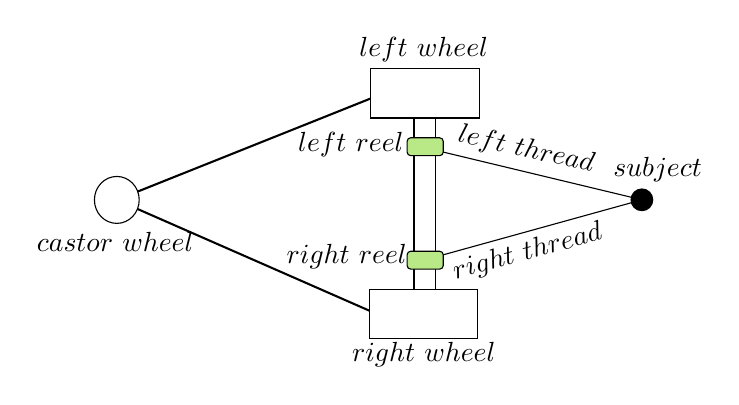
\begin{tikzpicture}[x=0.50pt,y=0.50pt,yscale=-1,xscale=1]
    %uncomment if require: \path (0,1774); %set diagram left start at 0, and has height of 1774
    %Shape: Rectangle [id:dp3163749047300972] 
    \draw   (341,1289.29) -- (356.46,1289.29) -- (356.46,1484.1) -- (341,1484.1) -- cycle ;
    %Straight Lines [id:da006917544597343617] 
    \draw [color={rgb, 255:red, 0; green, 0; blue, 0 }  ,draw opacity=1 ][line width=0.75]    (309.46,1464.29) -- (126.19,1383.9) ;
    
    
    %Straight Lines [id:da6556986586628986] 
    \draw [color={rgb, 255:red, 0; green, 0; blue, 0 }  ,draw opacity=1 ][fill={rgb, 255:red, 230; green, 164; blue, 164 }  ,fill opacity=1 ][line width=0.75]    (310.46,1310.29) -- (126.19,1383.9) ;
    
    
    %Shape: Rectangle [id:dp7070304476532343] 
    \draw  [fill={rgb, 255:red, 255; green, 255; blue, 255 }  ,fill opacity=1 ] (309.5,1289) -- (388,1289) -- (388,1324.67) -- (309.5,1324.67) -- cycle ;
    %Shape: Ellipse [id:dp4674581553313458] 
    \draw  [color={rgb, 255:red, 0; green, 0; blue, 0 }  ,draw opacity=1 ][fill={rgb, 255:red, 255; green, 255; blue, 255 }  ,fill opacity=1 ] (110.01,1383.9) .. controls (110.01,1374.53) and (117.25,1366.94) .. (126.19,1366.94) .. controls (135.12,1366.94) and (142.37,1374.53) .. (142.37,1383.9) .. controls (142.37,1393.28) and (135.12,1400.87) .. (126.19,1400.87) .. controls (117.25,1400.87) and (110.01,1393.28) .. (110.01,1383.9) -- cycle ;
    %Shape: Rectangle [id:dp46270765707902994] 
    \draw  [fill={rgb, 255:red, 255; green, 255; blue, 255 }  ,fill opacity=1 ] (308.5,1448.5) -- (387,1448.5) -- (387,1484.17) -- (308.5,1484.17) -- cycle ;
    %Shape: Circle [id:dp1556138070188774] 
    \draw  [fill={rgb, 255:red, 0; green, 0; blue, 0 }  ,fill opacity=1 ] (497.83,1383.83) .. controls (497.83,1379.51) and (501.34,1376) .. (505.67,1376) .. controls (509.99,1376) and (513.5,1379.51) .. (513.5,1383.83) .. controls (513.5,1388.16) and (509.99,1391.67) .. (505.67,1391.67) .. controls (501.34,1391.67) and (497.83,1388.16) .. (497.83,1383.83) -- cycle ;
    %Straight Lines [id:da9759075394788362] 
    \draw    (362.11,1349.34) -- (505.67,1383.83) ;
    
    
    %Straight Lines [id:da0292648785573405] 
    \draw    (362.11,1423.58) -- (429.74,1404.86) -- (505.67,1383.83) ;
    
    
    %Rounded Rect [id:dp19413777874284577] 
    \draw  [color={rgb, 255:red, 0; green, 0; blue, 0 }  ,draw opacity=1 ][fill={rgb, 255:red, 184; green, 233; blue, 134 }  ,fill opacity=1 ] (336,1423.58) .. controls (336,1422.16) and (337.16,1421) .. (338.58,1421) -- (359.53,1421) .. controls (360.96,1421) and (362.11,1422.16) .. (362.11,1423.58) -- (362.11,1431.34) .. controls (362.11,1432.76) and (360.96,1433.92) .. (359.53,1433.92) -- (338.58,1433.92) .. controls (337.16,1433.92) and (336,1432.76) .. (336,1431.34) -- cycle ;
    %Rounded Rect [id:dp9015992902460356] 
    \draw  [color={rgb, 255:red, 0; green, 0; blue, 0 }  ,draw opacity=1 ][fill={rgb, 255:red, 184; green, 233; blue, 134 }  ,fill opacity=1 ] (336,1341.58) .. controls (336,1340.16) and (337.16,1339) .. (338.58,1339) -- (359.53,1339) .. controls (360.96,1339) and (362.11,1340.16) .. (362.11,1341.58) -- (362.11,1349.34) .. controls (362.11,1350.76) and (360.96,1351.92) .. (359.53,1351.92) -- (338.58,1351.92) .. controls (337.16,1351.92) and (336,1350.76) .. (336,1349.34) -- cycle ;
    
    % Text Node
    \draw  [draw opacity=0][fill={rgb, 255:red, 255; green, 255; blue, 255 }  ,fill opacity=1 ]  (478.5,1350) -- (535.5,1350) -- (535.5,1374) -- (478.5,1374) -- cycle  ;
    \draw (517,1362) node    {$subject$};
    % Text Node
    \draw (302,1344) node    {$left\ reel\  \ $};
    % Text Node
    \draw (299,1425) node    {$right\ reel\  \ $};
    % Text Node
    \draw (125,1414) node    {$castor\ wheel$};
    % Text Node
    \draw (422,1348) node  [rotate=-12.55]  {$left\ thread$};
    % Text Node
    \draw (423,1422) node  [rotate=-344.79]  {$right\ thread$};
    % Text Node
    \draw (348,1275) node    {$left\ wheel$};
    % Text Node
    \draw (348,1496) node    {$right\ wheel$};
    \end{tikzpicture}
    \caption{Components of the robotic vehicle and the tether mechanism}
    \label{fig:components}
\end{figure}{}


The proposed solution is a Differential-Wheeled Robot (DWR) tethered to the followed subject with two threads ending at a single point attached to the subject waist, back or hand. In the same axis as the two front wheels, the robot has two reels separated by a certain length from which these threads come. As the subject moves away from the robot, the reels release thread so that the patient does not physically drag the vehicle. When the opposite happens, and the vehicle gets closer to the subject, an active spring mechanism driven by electric motors move each reel to retract the thread. The threads need to be tense at all times so that the encoders in each reel can be used to continuously measure the distance between the subject and the reel as devised in Figure~\ref{fig:components}.

% El detalle de los encoders se puede eliminar, es info común.
Encoders in each reel measure the difference in length of each thread compared to its initial position. These differences in length are the input for the control algorithm.  Using the encoder, the difference in length for each thread can be measured with Equations~\ref{eq:encoder_len}.

\begin{equation}
\label{eq:encoder_len}
\begin{array}{ll}  
l_L = pulses_{l} \; \frac{2\pi r}{ppr}  \\
\\
l_R = pulses_{r} \; \frac{2\pi r}{ppr}
\end{array}
\end{equation}{}

\noindent where $pulses_{l}$ and $pulses_{r}$ are the pulses obtained for the left and right encoder.  Pulses refer to natural discrete numbers that represents the circular movement of the encoder shaft.  The variable $r$ is the radius of the reel and $ppr$ is the pulses per revolution (resolution) of the encoder. These equations provide the estimated values for the left $l_L$ and right $l_R$, which are the length of thread released from each reel.   The initial position of the threads is configurable.

\subsection{Hardware}

\begin{figure}[h!]
\centering
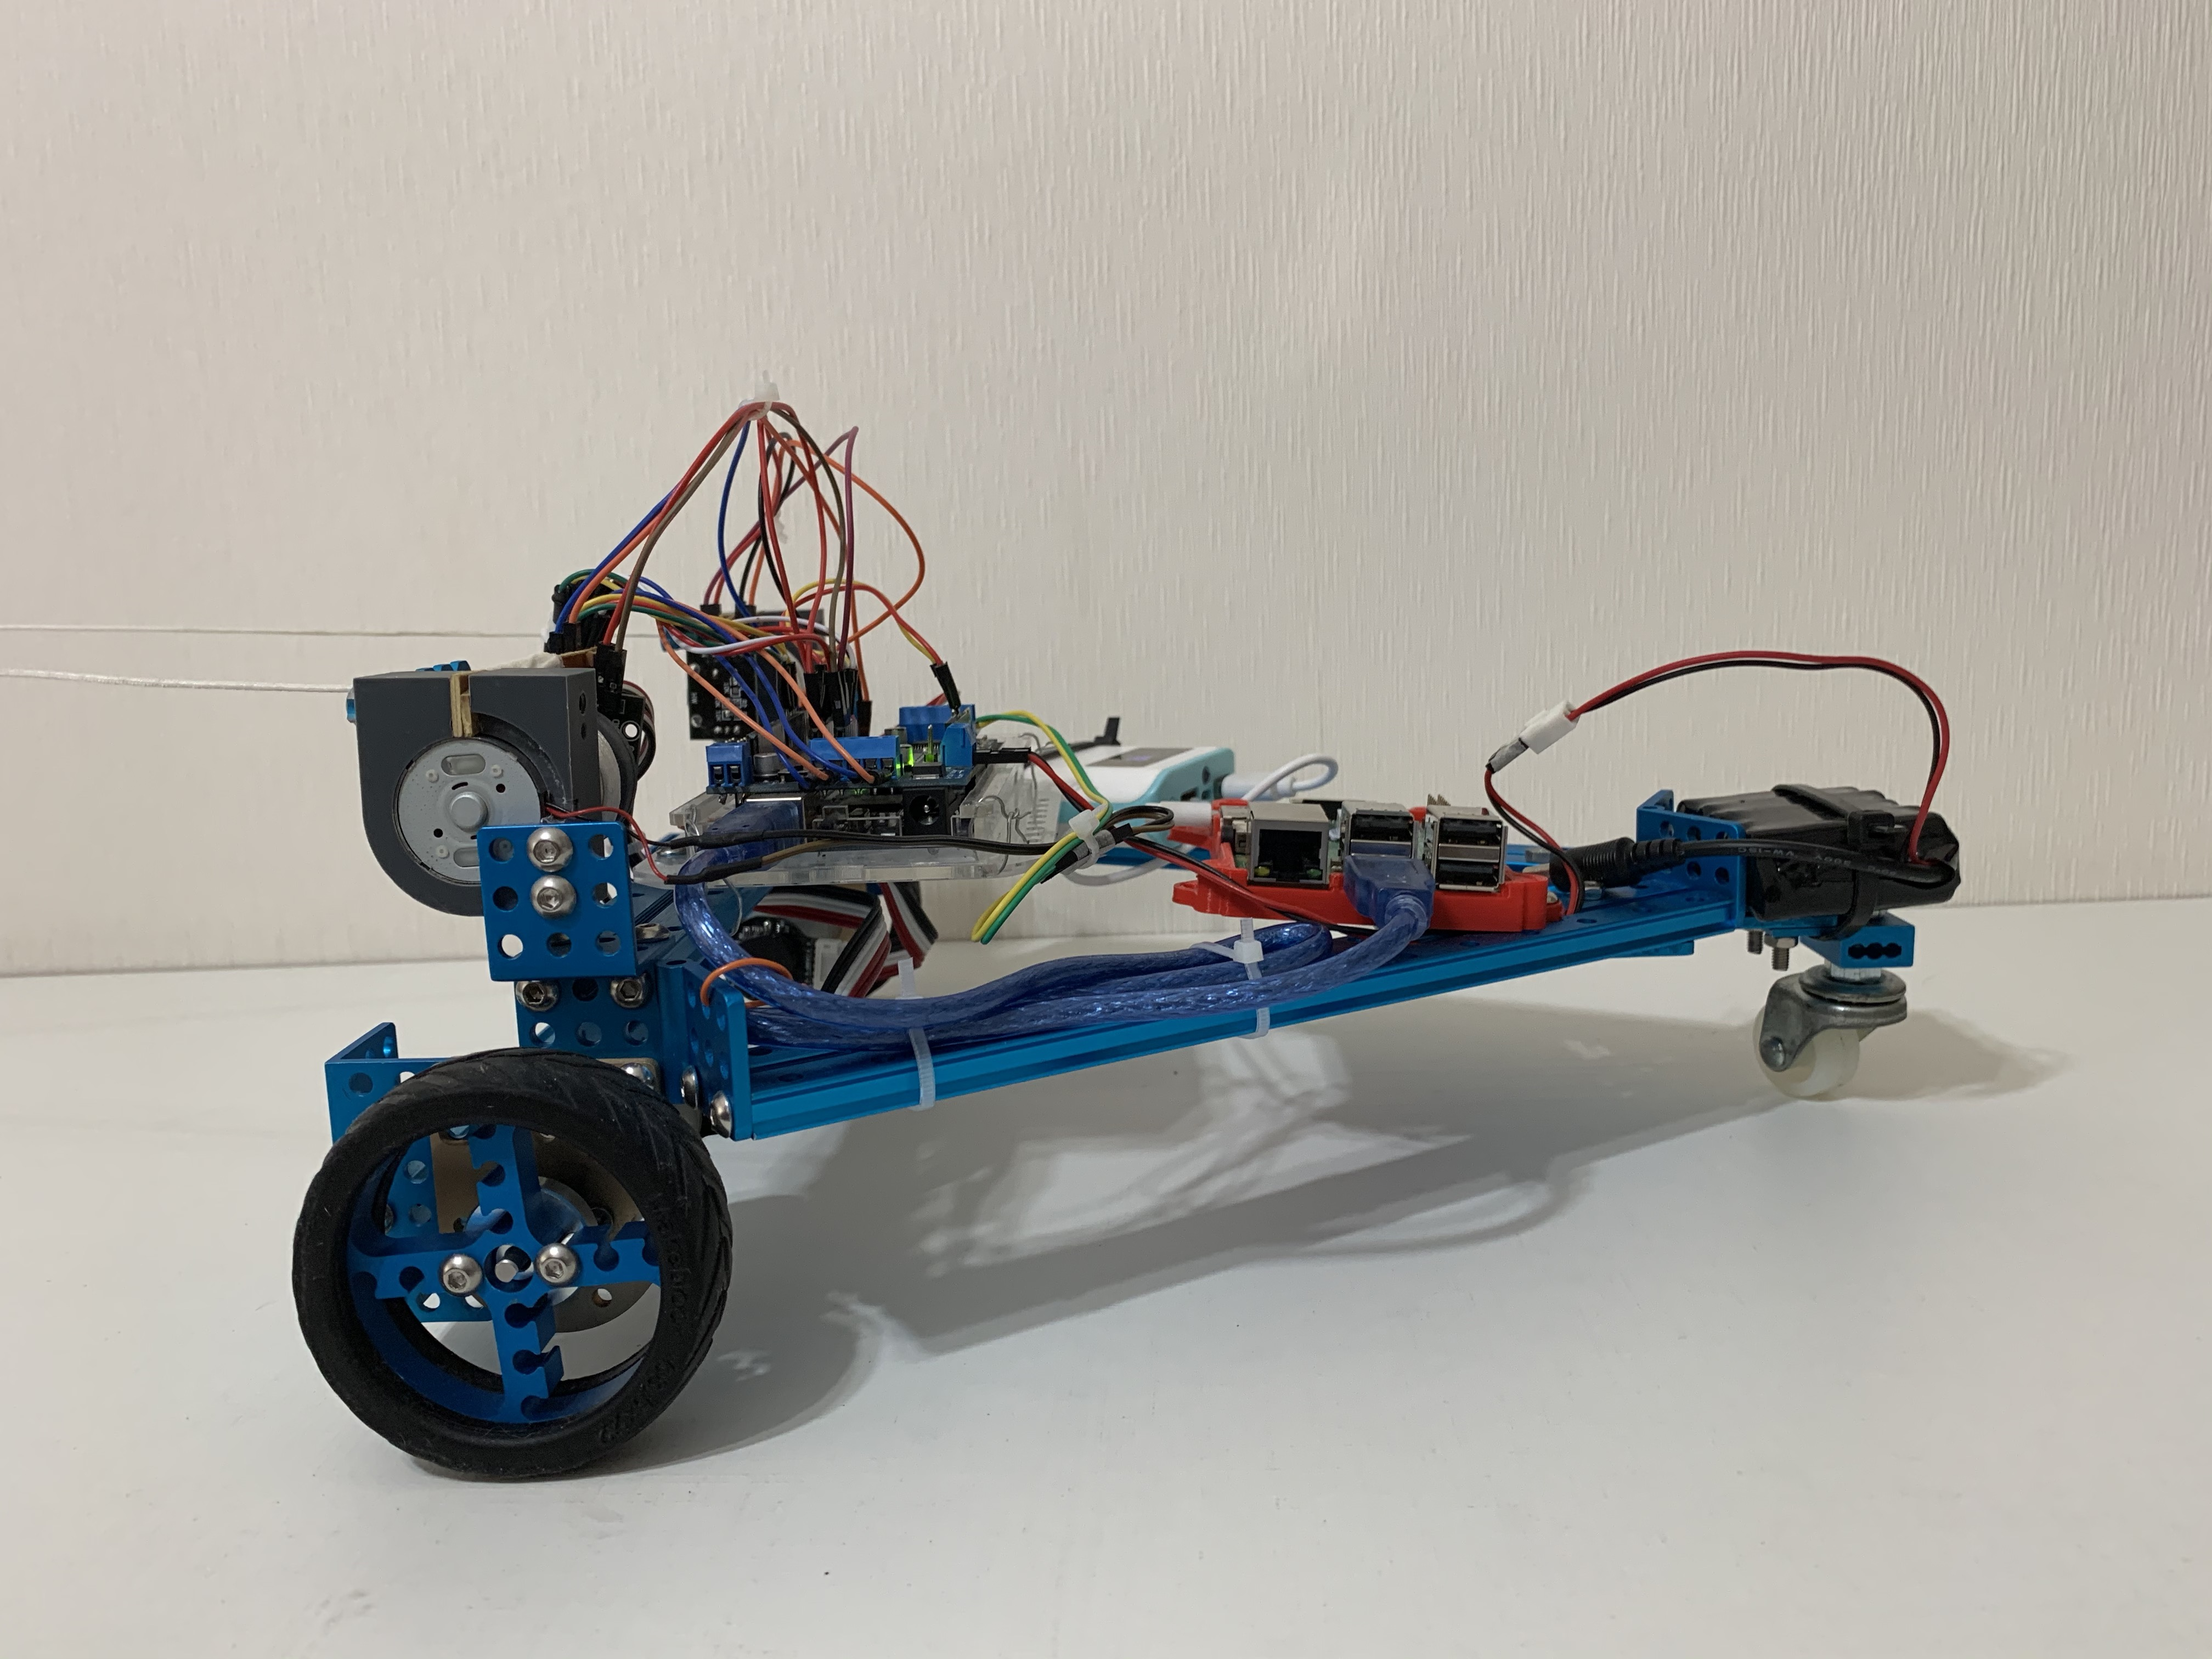
\includegraphics[width=8cm]{images/alpibot1.jpg}
\caption{Side-view of the robot prototype.  A differential wheel, the reel and the rear free castor wheel can be observed from the picture.}
\label{fig:alpibot1}
\end{figure}


Frames are constructed from aluminum extrusions produced by Makeblock (Shenzhen, China).   The prototype is a three-wheeled robot with two frontal differential drive wheels and a free castor wheel as a third point of contact on the back, as can be seen on Figures~\ref{fig:alpibot1} and~\ref{fig:alpibot2}.  

Two motors Makeblock Optical Encoder Motor-25 9V/86 rpm are used on in-wheel configuration providing optical encoding.  A microcontroller Arduino (Arduino LLC, Italy) Mega 2560 is used to implement the control loop and to provide encoder processing.  On top of it an Adafruit (Adafruit, New York City) Motor Shield v2 bridge is used to drive the four DC motors, one for each wheel and one on each reel.   The Arduino board is also connected to a Single Board Computer (SBC) Raspberry Pi (Raspberry Pi Foundation, United Kingdom) 3B+ through serial connection on one of the USB port.

\begin{figure*}[!t]
\centering
\subfloat{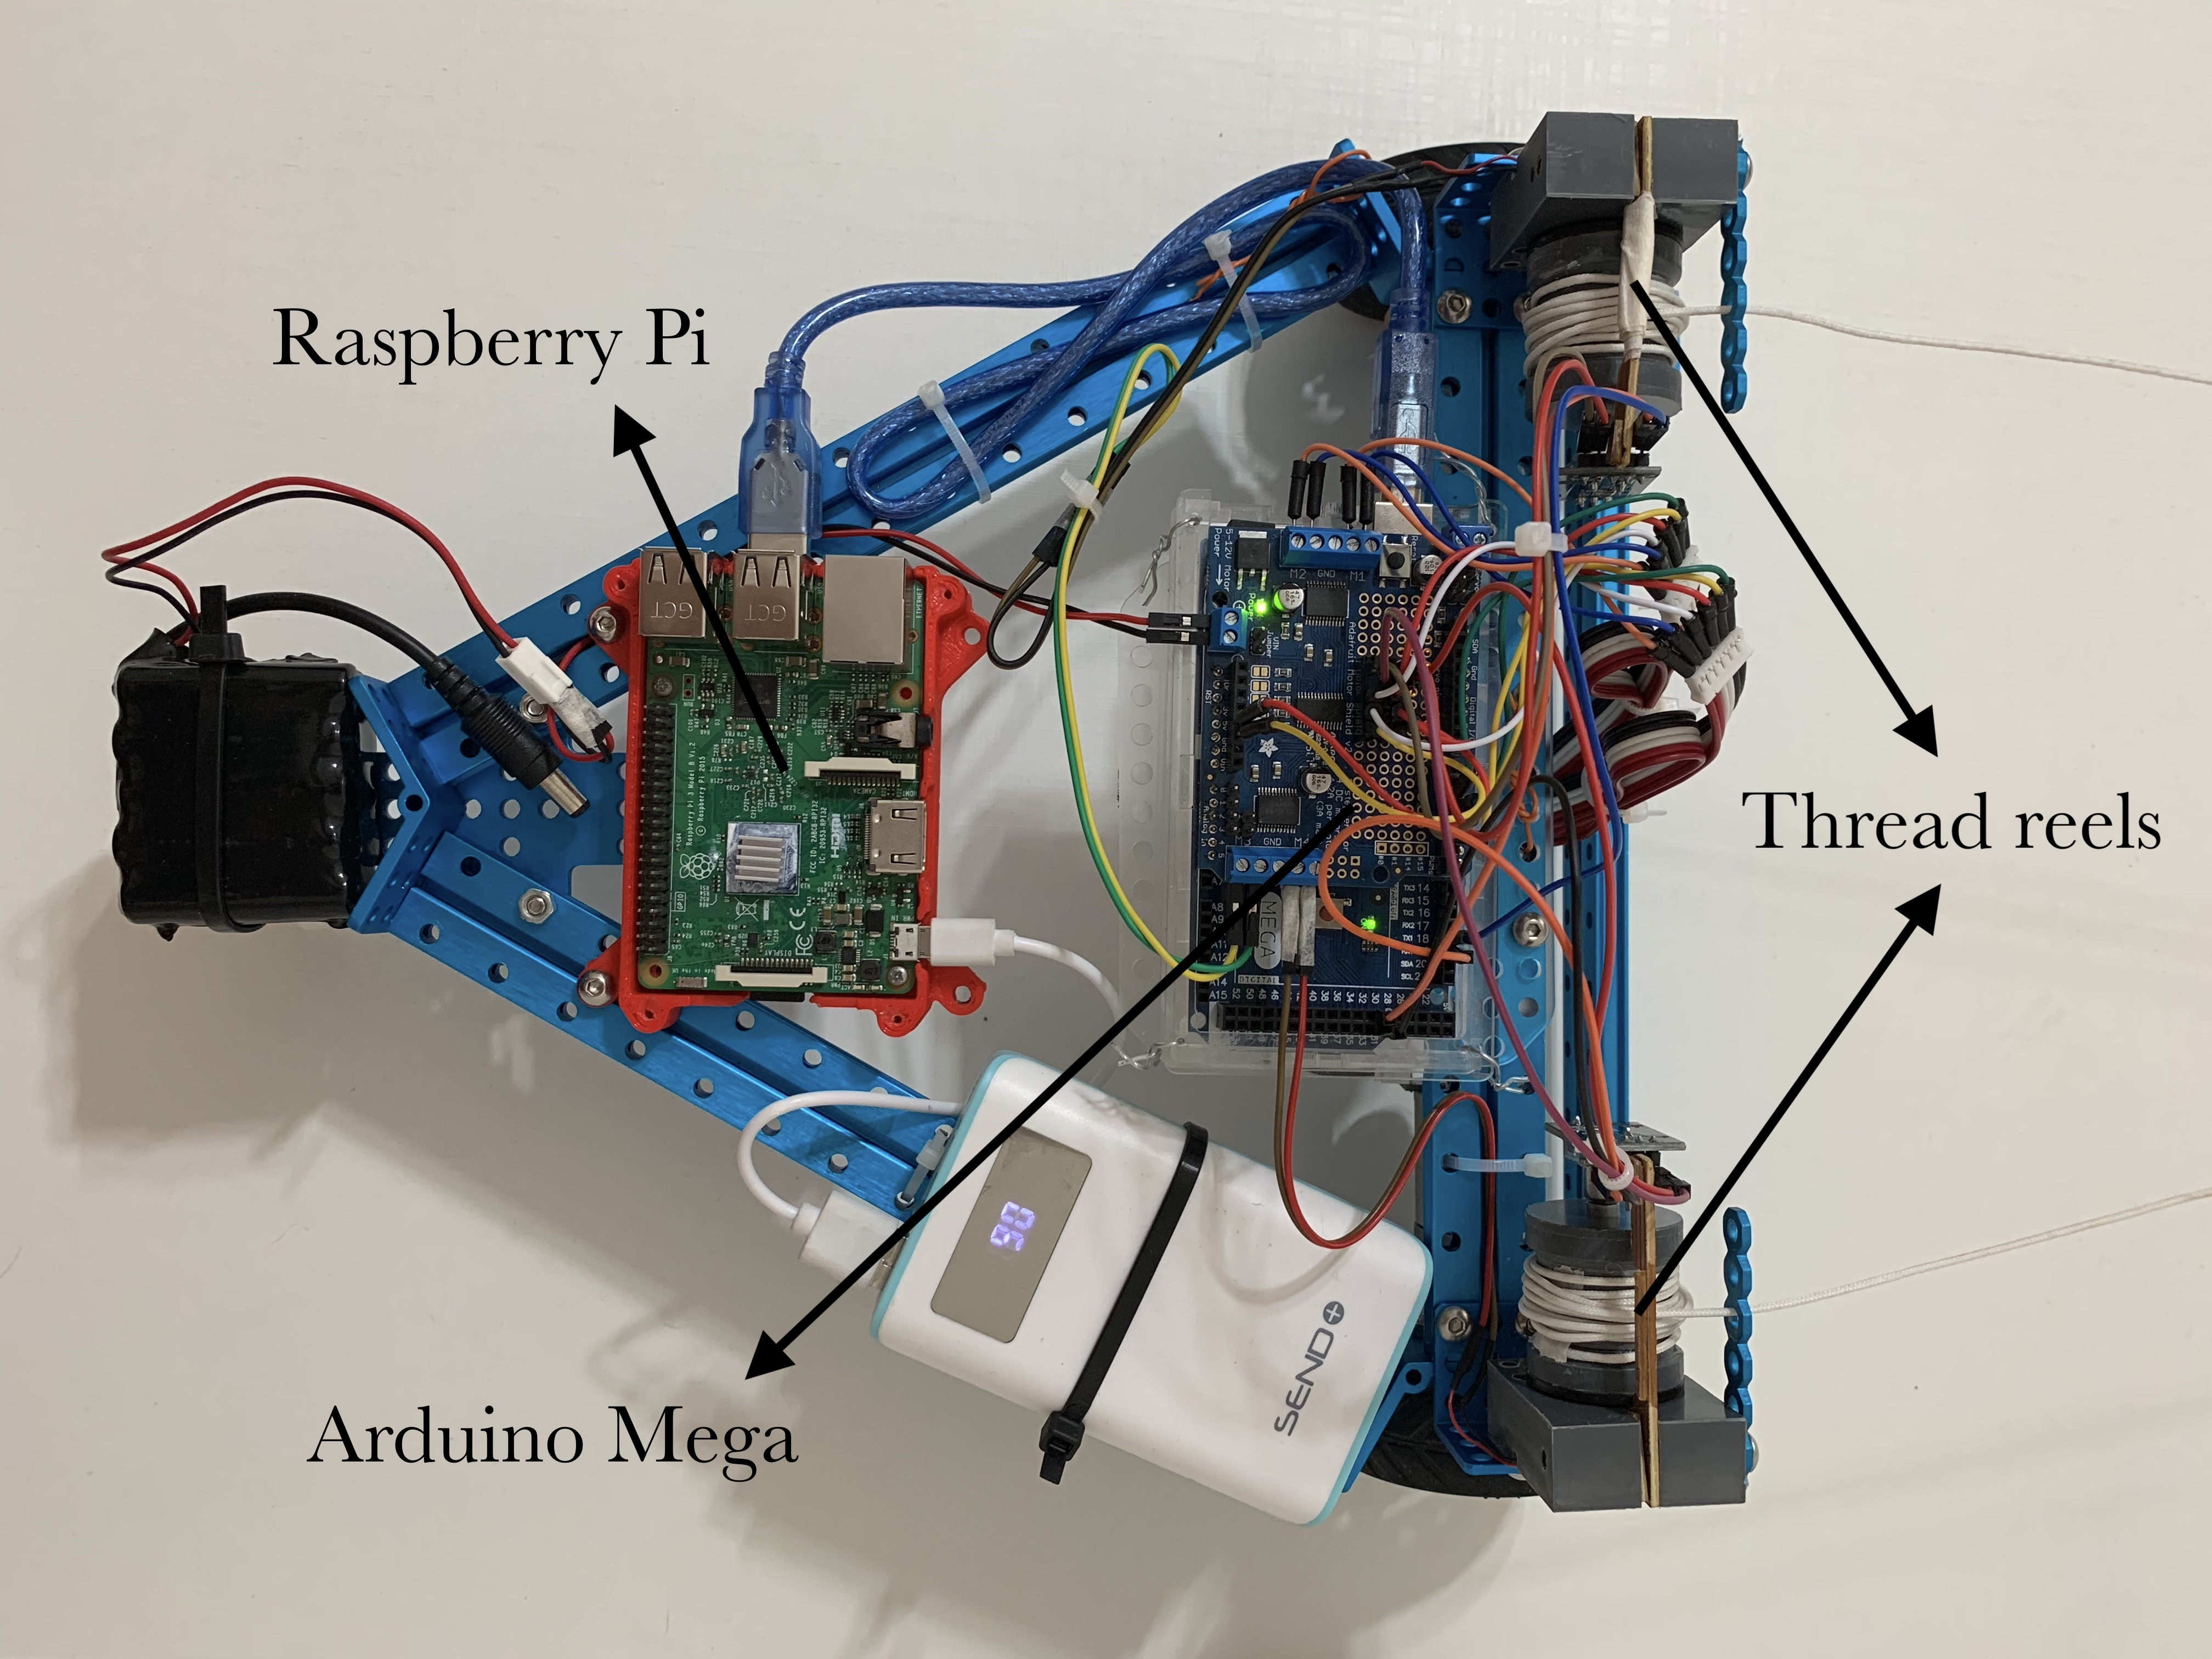
\includegraphics[width=15cm]{images/alpibot2.jpg}\label{subject8}}
\caption{Top view of the robot prototype.  The SBC is shown on the center, alongside the Arduino Mega board.  Both reels can be seen on the same vertical plane of the wheel axis. A power bank (white) is located on one side of the robot, and on the rear part, the motor power battery (black) is located.}
\label{fig:alpibot2}
\end{figure*}

The SBC connects to a WiFi network and can receive remote commands to control the robot. It also broadcasts telemetry data to any listening devices on the network. The control algorithms run in this board, which continuously communicates with the Arduino board to receive sensor data and to issue commands to move the motors or retract the reels.   The algorithms are programmed in Python 3.7, which allows the exact same code to run both the simulated and real world prototype.  


%The microcontroller is connected through serial connection to the main SBC RaspberryPi Model 3B+.  The main controlling algorithm run on this board, it connects to wifi and provides telemetry and the abiilty to receive remote commands by means a very simple UDP command interface.

The two reels are designed from PVC extrusions and are shown on Figure~\ref{fig:alpibot2}.  They are attached to regular FA-12350 DC motors scavenged from old compact discs.  Each reel is axially locked to inexpensive Ky-040 rotary encoder~\cite{SugaharaJunOnoKoji1998} which provides around 20 pulses per revolution.
%Hardware specifications are described on table \ref{tab:specifications}.

The prototype can be seen on Figure~\ref{fig:alpibot1} and~\ref{fig:alpibot2}.  It has two separate batteries, one powering the Raspberry Pi, the Arduino board and the encoder electronics, and the other powering the drive and reel motors. The first battery is a commercial power bank with a capacity of 10000 mA$\cdot$h, and an output of 3.1A (over two USB ports) at 5V. The motor battery is a set of 10 AAA nickel–metal hydride batteries (1.2V each), with a total output of 12V.  

\subsection{Active Reel Spring}

As previously mentioned, an active spring~\cite{Vanderborght2013} mechanism is also put in place to keep the threads tense.  However, in order to extend the useful life of the reel motors, and to save battery, an algorithm to  activate and deactivate the motors was developed. 

The algorithm works as follows: 

\begin{enumerate}
    \item While wheels are moving, retract reels.
    \item If wheels stop moving, wait for \textit{reel wait time} seconds, then retract reels. 
    \item Retract reels until the reel encoders values have not changed during \textit{reel retract time} seconds.
    \item If wheels started moving or the encoder values have changed while retracting, start the \textit{reel retract time} countdown again.
\end{enumerate}{}

%Here is the pseudocode that implements that logic. This function is executed in every run loop in the Arduino module:


%\begin{algorithm}[]
%\label{alg:active_spring}
%\caption{Active spring algorithm}
%\begin{algorithmic}
%
%\STATE $currentReelPulses \gets readPulses()$
%
%\IF{$retracting$}
%    \IF{$lastReelPulses != currentReelPulses$}
%    \STATE $lastReelStart \gets currentTime()$
%    \ENDIF
%    \IF{\NOT $ wheelsMoving $ \AND $ currentTime() - lastReelStart > rrt$}
%    \STATE $retracting \gets \FALSE$
%    \STATE $lastReelEnd \gets currentTime()$
%    \ENDIF
%\ELSE
%    \IF{$wheelsMoving$}
%        \STATE $retracting \gets \TRUE$
%        \STATE $lastReelStart \gets currentTime()$
%    \ENDIF
%    \IF{$ currentTime() - lastReelEnd > rwt $}
%        \STATE $retracting \gets \TRUE$
%        \STATE $lastReelStart \gets currentTime()$
%    \ENDIF
%\ENDIF
%
%\STATE $lastReelPulses \gets currentReelPulses$
%
%\IF{$retracting$}
%    \STATE \textit{Activate reel motors}
%\ELSE
%    \STATE \textit{Deactivate reel motors}
%\ENDIF
%\end{algorithmic}
%\end{algorithm}


%\subsection{Software Components}

\subsection{Control Strategy}

Two simple algorithmic control strategies are proposed and evaluated.  The first one is called \textit{Follow the thread} and the second strategy is \textit{Rotate and go}.  %The Adafruit Shield controller provides a very stable output signal, provided battery are kept above reference.  Hence, wheels motor control is open-loop.

\subsubsection{Follow the Thread}

This control strategy is similar to the one presented in \cite{Ortlieb2016}.  It is based on the idea that both the relative angle between the subject and the vehicle orientation and, the relative distance between the robot and the subject, can be computed from the length of the left and right threads.  They are described by Equations~\ref{eq:lemniscata}, \ref{eq:lemniscata2} and~\ref{eq:lemniscata3}.

\begin{equation}
V_t = c_v (\frac{l_L + l_R}{2} - l_D)
\label{eq:lemniscata}
\end{equation}

\begin{equation}
\omega_{L} = V_t + c_{\alpha} (l_L - l_R)
\label{eq:lemniscata2}
\end{equation}

\begin{equation}
\omega_{R} = V_t - c_{\alpha} (l_L - l_R)
\label{eq:lemniscata3}
\end{equation}

\noindent where  $c_v$ and $c_{\alpha}$ are constant coefficients used for calibration whose units are expressed in $[\frac{1}{s}]$, and $l_D$ is a constant offset in $[m]$ that is used to customize the desired length of the thread where the robot does not move.   As shown on Figure~\ref{fig:follow_params},  $l_L$ and $l_R$ are changes in the length of thread that was released from each reel in $[m]$  obtained from encoder information from Equation~\ref{eq:encoder_len}, $V_t$ is the estimated forward velocity for the target and finally $\omega_{L}$ are $\omega_{R}$ are the velocity values that are directly used to drive each wheel motor.

To stop the vehicle completely when it is close to its expected position, an additional condition is added: 

\begin{equation}
\textit{if  }{\frac{l_L + l_R}{2} < l_D}\textit{ then } \omega_{L} = \omega_{R} = 0.
\end{equation}

\begin{figure}[]
    \centering
    \tikzset{every picture/.style={line width=0.75pt}} %set default line width to 0.75pt        
    
    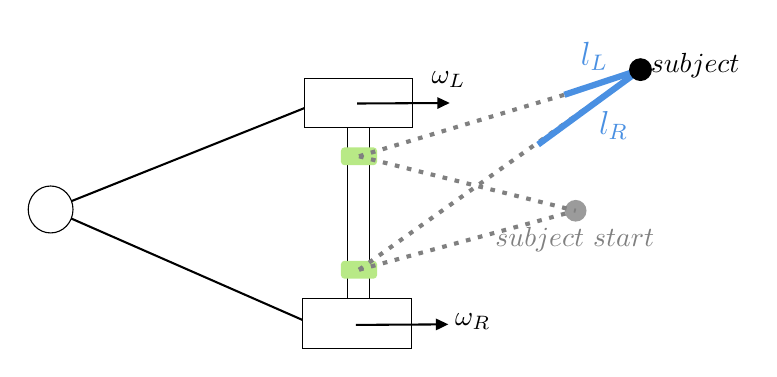
\begin{tikzpicture}[x=0.50pt,y=0.50pt,yscale=-1,xscale=1]
    %uncomment if require: \path (0,2317); %set diagram left start at 0, and has height of 2317
    
    %Shape: Rectangle [id:dp785217180323701] 
    \draw   (332,1925.29) -- (347.46,1925.29) -- (347.46,2120.1) -- (332,2120.1) -- cycle ;
    %Straight Lines [id:da8987873257842873] 
    \draw [color={rgb, 255:red, 0; green, 0; blue, 0 }  ,draw opacity=1 ][line width=0.75]    (300.46,2100.29) -- (117.19,2019.9) ;
    %Straight Lines [id:da585150688871364] 
    \draw [color={rgb, 255:red, 0; green, 0; blue, 0 }  ,draw opacity=1 ][fill={rgb, 255:red, 230; green, 164; blue, 164 }  ,fill opacity=1 ][line width=0.75]    (301.46,1946.29) -- (117.19,2019.9) ;
    %Shape: Rectangle [id:dp8556526042433679] 
    \draw  [fill={rgb, 255:red, 255; green, 255; blue, 255 }  ,fill opacity=1 ] (300.5,1925) -- (379,1925) -- (379,1960.67) -- (300.5,1960.67) -- cycle ;
    %Shape: Ellipse [id:dp024503202773356936] 
    \draw  [color={rgb, 255:red, 0; green, 0; blue, 0 }  ,draw opacity=1 ][fill={rgb, 255:red, 255; green, 255; blue, 255 }  ,fill opacity=1 ] (101.01,2019.9) .. controls (101.01,2010.53) and (108.25,2002.94) .. (117.19,2002.94) .. controls (126.12,2002.94) and (133.37,2010.53) .. (133.37,2019.9) .. controls (133.37,2029.28) and (126.12,2036.87) .. (117.19,2036.87) .. controls (108.25,2036.87) and (101.01,2029.28) .. (101.01,2019.9) -- cycle ;
    %Shape: Rectangle [id:dp4521863424396907] 
    \draw  [fill={rgb, 255:red, 255; green, 255; blue, 255 }  ,fill opacity=1 ] (299.5,2084.5) -- (378,2084.5) -- (378,2120.17) -- (299.5,2120.17) -- cycle ;
    %Rounded Rect [id:dp9798921511906625] 
    \draw  [draw opacity=0][fill={rgb, 255:red, 184; green, 233; blue, 134 }  ,fill opacity=1 ] (327,2059.58) .. controls (327,2058.16) and (328.16,2057) .. (329.58,2057) -- (350.53,2057) .. controls (351.96,2057) and (353.11,2058.16) .. (353.11,2059.58) -- (353.11,2067.34) .. controls (353.11,2068.76) and (351.96,2069.92) .. (350.53,2069.92) -- (329.58,2069.92) .. controls (328.16,2069.92) and (327,2068.76) .. (327,2067.34) -- cycle ;
    %Rounded Rect [id:dp969028519585216] 
    \draw  [draw opacity=0][fill={rgb, 255:red, 184; green, 233; blue, 134 }  ,fill opacity=1 ] (327,1977.58) .. controls (327,1976.16) and (328.16,1975) .. (329.58,1975) -- (350.53,1975) .. controls (351.96,1975) and (353.11,1976.16) .. (353.11,1977.58) -- (353.11,1985.34) .. controls (353.11,1986.76) and (351.96,1987.92) .. (350.53,1987.92) -- (329.58,1987.92) .. controls (328.16,1987.92) and (327,1986.76) .. (327,1985.34) -- cycle ;
    %Straight Lines [id:da8580549640030513] 
    \draw [color={rgb, 255:red, 128; green, 128; blue, 128 }  ,draw opacity=1 ][line width=1.5]  [dash pattern={on 1.69pt off 2.76pt}]  (340.06,2063.46) -- (496.67,2020.83) ;
    %Shape: Circle [id:dp1613016595870852] 
    \draw  [draw opacity=0][fill={rgb, 255:red, 155; green, 155; blue, 155 }  ,fill opacity=1 ] (488.83,2020.83) .. controls (488.83,2016.51) and (492.34,2013) .. (496.67,2013) .. controls (500.99,2013) and (504.5,2016.51) .. (504.5,2020.83) .. controls (504.5,2025.16) and (500.99,2028.67) .. (496.67,2028.67) .. controls (492.34,2028.67) and (488.83,2025.16) .. (488.83,2020.83) -- cycle ;
    %Straight Lines [id:da10232028406547378] 
    \draw [color={rgb, 255:red, 0; green, 0; blue, 0 }  ,draw opacity=1 ][line width=0.75]    (338.75,1943.33) -- (402.58,1942.95) ;
    \draw [shift={(405.58,1942.93)}, rotate = 539.65] [fill={rgb, 255:red, 0; green, 0; blue, 0 }  ,fill opacity=1 ][line width=0.08]  [draw opacity=0] (8.93,-4.29) -- (0,0) -- (8.93,4.29) -- cycle    ;
    %Straight Lines [id:da5543519847675118] 
    \draw [color={rgb, 255:red, 0; green, 0; blue, 0 }  ,draw opacity=1 ][line width=0.75]    (337.75,2103.33) -- (401.58,2102.95) ;
    \draw [shift={(404.58,2102.93)}, rotate = 539.65] [fill={rgb, 255:red, 0; green, 0; blue, 0 }  ,fill opacity=1 ][line width=0.08]  [draw opacity=0] (8.93,-4.29) -- (0,0) -- (8.93,4.29) -- cycle    ;
    %Straight Lines [id:da5830729933065488] 
    \draw [color={rgb, 255:red, 128; green, 128; blue, 128 }  ,draw opacity=1 ][line width=1.5]  [dash pattern={on 1.69pt off 2.76pt}]  (340.06,1981.46) -- (496.67,2020.83) ;
    %Straight Lines [id:da27552399356884627] 
    \draw [color={rgb, 255:red, 128; green, 128; blue, 128 }  ,draw opacity=1 ][line width=1.5]  [dash pattern={on 1.69pt off 2.76pt}]  (340.06,1981.46) -- (488.5,1937) ;
    %Straight Lines [id:da06167712807711301] 
    \draw [color={rgb, 255:red, 128; green, 128; blue, 128 }  ,draw opacity=1 ][line width=1.5]  [dash pattern={on 1.69pt off 2.76pt}]  (340.06,2063.46) -- (543.5,1918.83) ;
    %Straight Lines [id:da887785453759708] 
    \draw [color={rgb, 255:red, 74; green, 144; blue, 226 }  ,draw opacity=1 ][line width=2.25]    (488.5,1937) -- (543.5,1918.83) ;
    %Straight Lines [id:da7211287180458504] 
    \draw [color={rgb, 255:red, 74; green, 144; blue, 226 }  ,draw opacity=1 ][line width=2.25]    (469.5,1973) -- (543.5,1918.83) ;
    %Shape: Circle [id:dp7802267148020259] 
    \draw  [fill={rgb, 255:red, 0; green, 0; blue, 0 }  ,fill opacity=1 ] (535.67,1918.83) .. controls (535.67,1914.51) and (539.17,1911) .. (543.5,1911) .. controls (547.83,1911) and (551.33,1914.51) .. (551.33,1918.83) .. controls (551.33,1923.16) and (547.83,1926.67) .. (543.5,1926.67) .. controls (539.17,1926.67) and (535.67,1923.16) .. (535.67,1918.83) -- cycle ;
    
    % Text Node
    \draw (524,1960) node  [font=\large,color={rgb, 255:red, 74; green, 144; blue, 226 }  ,opacity=1 ]  {$ \begin{array}{l}
    l_{R}\\
    \end{array}$};
    % Text Node
    \draw (510,1910) node  [font=\large,color={rgb, 255:red, 74; green, 144; blue, 226 }  ,opacity=1 ,rotate=-358.27]  {$ \begin{array}{l}
    l_{L}\\
    \end{array}$};
    % Text Node
    \draw (496,2042) node  [color={rgb, 255:red, 128; green, 128; blue, 128 }  ,opacity=1 ]  {$subject\ start$};
    % Text Node
    \draw  [draw opacity=0][fill={rgb, 255:red, 255; green, 255; blue, 255 }  ,fill opacity=1 ]  (554.5,1904) -- (611.5,1904) -- (611.5,1928) -- (554.5,1928) -- cycle  ;
    \draw (583,1916) node    {$subject$};
    % Text Node
    \draw (390.58,1925.93) node [anchor=west] [inner sep=0.75pt]  [font=\normalsize,color={rgb, 255:red, 0; green, 0; blue, 0 }  ,opacity=1 ]  {$\omega_{L}$};
    % Text Node
    \draw (407.58,2100.93) node [anchor=west] [inner sep=0.75pt]  [font=\normalsize,color={rgb, 255:red, 0; green, 0; blue, 0 }  ,opacity=1 ]  {$\omega_{R}$};
    
    
    \end{tikzpicture}
    \caption{Following mechanism parameters}
    \label{fig:follow_params}
\end{figure}{}

\subsubsection{Rotate and Go}

The \textit{Rotate and go} algorithm divides the vehicle movement in two steps:

\begin{itemize}
\item Rotating the vehicle around the center point of the axis that connects its front wheels in order to aim at the subject.
\item Go forward in a straight line until the vehicle is at the expected distance to the subject.
\end{itemize}

The procedure is detailed in Algorithm~\ref{alg:rotateandgoalg}.  The variable $V_r$ is the speed at which the vehicle will rotate on its axis, and $V_f$ is the speed at which the vehicle will move forward once it can move on the subject's direction.  The algorithm requires three parameters, $c_v$ and $c_r$ that regulates the coefficients for the forward and rotation movement, and an additional parameter $Dt_{off}$ that regulates the sensibility of the rotation movement.  The constant parameter $Dm_{off}$ is similar to $l_D$, and is used to customize the length of the thread where the robot does not move at all. Temporary variables $Dt$ and $Dm$ are used in the algorithm to calculate the difference and the average of the changes in released thread. Lastly, $base_{vr}$, is another constant used to determine the minimum rotational velocity of the vehicle.


\begin{algorithm}[]
\caption{Rotate and go algorithm}
\begin{algorithmic}
\STATE \textbf{Define} $Dt \gets l_L - l_R$
\STATE \textbf{Define} $Dm \gets \frac{l_R+l_L}{2}$
\STATE $V_r \gets c_r * (abs(Dt) - Dt_{off}) + base_{vr}$ 
\STATE $V_f \gets c_v * (Dm - Dm_{off})$

\IF{$abs(Dt) > Dt_{off}$}
\IF{$l_L > l_R$}
\STATE $\omega_{L} \gets V_r$
\STATE $\omega_{R} \gets -V_r$
\ELSE
\STATE $\omega_{L} \gets -V_r$
\STATE $\omega_{R} \gets V_r$
\ENDIF

\ELSE
\IF{$D_m > Dm_{off}$}
\STATE $\omega_{R} \gets V_f$
\STATE $\omega_{L} \gets V_f$
\ELSE
\STATE $\omega_{R} \gets 0$
\STATE $\omega_{L} \gets 0$
\ENDIF
\ENDIF
\STATE Return $\omega_{R}$ and $\omega_{L}$.
\end{algorithmic}
\label{alg:rotateandgoalg}
\end{algorithm}

\section{Comparison with alternative methods} \label{Comparison}

\subsection{Equivalence between the single and double tethered system}

%\begin{figure}[h!]
%\centering
%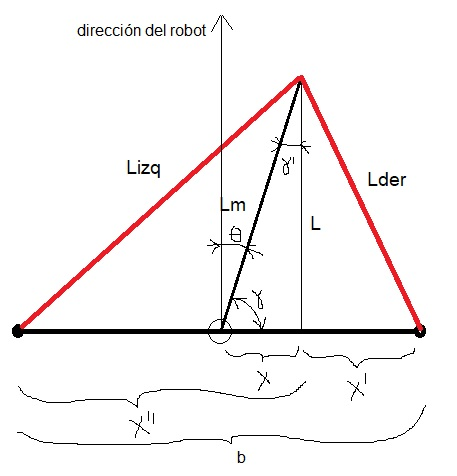
\includegraphics[width=8cm]{images/dibujito.jpg}
%\caption{Scheme of the equivalence between a single and dual thread systems.}
%\label{fig:dibujito}
%\end{figure}

In~\cite{Endo2015} authors propose a similar design based on only one thread.  They propose two control strategies based on two input parameters that are obtained from a linear and circular potentiometer that determines the length of the thread $l_m$ and the orientation angle $\theta$.  We show here that they are equivalent to the approach presented based on $l_L$ and  $l_R$.

Based on a frame reference with the robot on the center of coordinates as shown on Figure~\ref{fig:dibujitos}, from the input values $l_m$ and $\theta$ we can derive the position of the leader as

\begin{align*}
   y &= l_m  \cos(\theta)\\
   x &= l_m  \sin(\theta) \\
\end{align*}

%From the figure, it can be obtained that
%
%\begin{align*}
%x'            	&= \frac{b}{2}  - x \\
%x'' 			&= \frac{b}{2}  + x \\
%\end{align*}
%

\noindent where $x$ is the follower distance on the horizontal direction, and $y$ the follower distance on the vertical direction.

In this frame of reference, the lengths of the threads, $l_R$ and $l_L$ can be determined as


\begin{figure}[]
    \centering
    \tikzset{every picture/.style={line width=0.75pt}} %set default line width to 0.75pt            

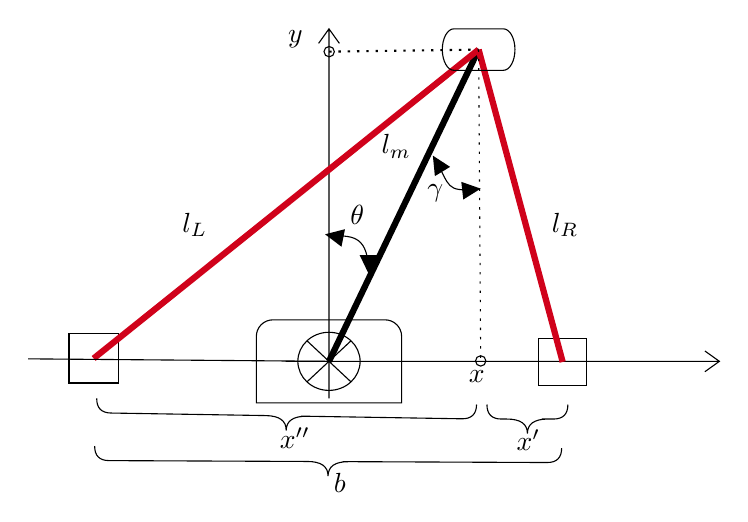
\begin{tikzpicture}[x=0.75pt,y=0.75pt,yscale=-1,xscale=1]
%uncomment if require: \path (0,235); %set diagram left start at 0, and has height of 235

%Shape: Axis 2D [id:dp7543865369052545] 
\draw  (312,162.89) -- (521,162.89)(332.9,2.69) -- (332.9,180.69) (514,157.89) -- (521,162.89) -- (514,167.89) (327.9,9.69) -- (332.9,2.69) -- (337.9,9.69)  ;
%Rounded Same Side Corner Rect [id:dp31787525316857024] 
\draw   (297.9,150.89) .. controls (297.9,146.47) and (301.48,142.89) .. (305.9,142.89) -- (359.9,142.89) .. controls (364.32,142.89) and (367.9,146.47) .. (367.9,150.89) -- (367.9,182.89) .. controls (367.9,182.89) and (367.9,182.89) .. (367.9,182.89) -- (297.9,182.89) .. controls (297.9,182.89) and (297.9,182.89) .. (297.9,182.89) -- cycle ;
%Shape: Square [id:dp8026938389823051] 
\draw   (434,151.69) -- (457,151.69) -- (457,174.69) -- (434,174.69) -- cycle ;
%Shape: Square [id:dp06857182701706144] 
\draw   (207.66,149.66) -- (231.34,149.66) -- (231.34,173.34) -- (207.66,173.34) -- cycle ;
%Flowchart: Summing Junction [id:dp2757072161924359] 
\draw   (317.9,162.89) .. controls (317.9,155.16) and (324.62,148.89) .. (332.9,148.89) .. controls (341.18,148.89) and (347.9,155.16) .. (347.9,162.89) .. controls (347.9,170.62) and (341.18,176.89) .. (332.9,176.89) .. controls (324.62,176.89) and (317.9,170.62) .. (317.9,162.89) -- cycle ; \draw   (322.29,152.99) -- (343.51,172.79) ; \draw   (343.51,152.99) -- (322.29,172.79) ;
%Straight Lines [id:da9717478160302964] 
\draw [line width=2.25]    (405,12.69) -- (332.9,162.89) ;
%Straight Lines [id:da30114532827552765] 
\draw [color={rgb, 255:red, 208; green, 2; blue, 27 }  ,draw opacity=1 ][line width=2.25]    (405,12.69) -- (219.5,161.5) ;
%Straight Lines [id:da0582330345196298] 
\draw [color={rgb, 255:red, 208; green, 2; blue, 27 }  ,draw opacity=1 ][line width=2.25]    (405,12.69) -- (445.5,163.19) ;
%Flowchart: Terminator [id:dp11720735085928635] 
\draw   (393.1,2.69) -- (416.9,2.69) .. controls (419.99,2.69) and (422.5,7.16) .. (422.5,12.69) .. controls (422.5,18.21) and (419.99,22.69) .. (416.9,22.69) -- (393.1,22.69) .. controls (390.01,22.69) and (387.5,18.21) .. (387.5,12.69) .. controls (387.5,7.16) and (390.01,2.69) .. (393.1,2.69) -- cycle ;
%Straight Lines [id:da6471016295019487] 
\draw  [dash pattern={on 0.84pt off 2.51pt}]  (405,12.69) -- (406,162.69) ;
%Shape: Circle [id:dp5568563915916713] 
\draw   (403.5,162.69) .. controls (403.5,161.31) and (404.62,160.19) .. (406,160.19) .. controls (407.38,160.19) and (408.5,161.31) .. (408.5,162.69) .. controls (408.5,164.07) and (407.38,165.19) .. (406,165.19) .. controls (404.62,165.19) and (403.5,164.07) .. (403.5,162.69) -- cycle ;
%Straight Lines [id:da6605293994654671] 
\draw    (188,161.69) -- (332.9,162.89) ;
%Shape: Brace [id:dp034761867026847026] 
\draw   (221,180.69) .. controls (220.93,185.36) and (223.22,187.73) .. (227.88,187.8) -- (302.39,189.02) .. controls (309.06,189.13) and (312.35,191.52) .. (312.27,196.19) .. controls (312.35,191.52) and (315.72,189.24) .. (322.38,189.35)(319.38,189.3) -- (396.89,190.57) .. controls (401.56,190.65) and (403.93,188.36) .. (404,183.69) ;
%Straight Lines [id:da6885647931399865] 
\draw [line width=0.75]  [dash pattern={on 0.84pt off 2.51pt}]  (333,13.69) -- (405,12.69) ;
%Curve Lines [id:da2681192753910786] 
\draw    (384.56,66.54) .. controls (391.15,78.31) and (389.42,81.22) .. (403.17,79.98) ;
\draw [shift={(406,79.69)}, rotate = 533.6600000000001] [fill={rgb, 255:red, 0; green, 0; blue, 0 }  ][line width=0.08]  [draw opacity=0] (8.93,-4.29) -- (0,0) -- (8.93,4.29) -- cycle    ;
\draw [shift={(382.95,63.79)}, rotate = 58.73] [fill={rgb, 255:red, 0; green, 0; blue, 0 }  ][line width=0.08]  [draw opacity=0] (8.93,-4.29) -- (0,0) -- (8.93,4.29) -- cycle    ;
%Curve Lines [id:da7846164710785513] 
\draw    (334.02,102.11) .. controls (342.64,102.92) and (351.11,101.09) .. (351.93,117.88) ;
\draw [shift={(352,120.69)}, rotate = 270] [fill={rgb, 255:red, 0; green, 0; blue, 0 }  ][line width=0.08]  [draw opacity=0] (8.93,-4.29) -- (0,0) -- (8.93,4.29) -- cycle    ;
\draw [shift={(331,101.69)}, rotate = 11.31] [fill={rgb, 255:red, 0; green, 0; blue, 0 }  ][line width=0.08]  [draw opacity=0] (8.93,-4.29) -- (0,0) -- (8.93,4.29) -- cycle    ;
%Shape: Brace [id:dp8659813161256731] 
\draw   (220,203.69) .. controls (219.98,208.36) and (222.3,210.7) .. (226.97,210.72) -- (322.47,211.13) .. controls (329.14,211.16) and (332.46,213.51) .. (332.44,218.18) .. controls (332.46,213.51) and (335.8,211.19) .. (342.47,211.22)(339.47,211.21) -- (437.97,211.64) .. controls (442.64,211.66) and (444.98,209.34) .. (445,204.67) ;
%Shape: Brace [id:dp4829292799998628] 
\draw   (409,183.69) .. controls (409,188.36) and (411.33,190.69) .. (416,190.69) -- (418.5,190.69) .. controls (425.17,190.69) and (428.5,193.02) .. (428.5,197.69) .. controls (428.5,193.02) and (431.83,190.69) .. (438.5,190.69)(435.5,190.69) -- (441,190.69) .. controls (445.67,190.69) and (448,188.36) .. (448,183.69) ;
%Shape: Circle [id:dp5543776560649496] 
\draw   (330.5,13.69) .. controls (330.5,12.31) and (331.62,11.19) .. (333,11.19) .. controls (334.38,11.19) and (335.5,12.31) .. (335.5,13.69) .. controls (335.5,15.07) and (334.38,16.19) .. (333,16.19) .. controls (331.62,16.19) and (330.5,15.07) .. (330.5,13.69) -- cycle ;

% Text Node
\draw (399,166.09) node [anchor=north west][inner sep=0.75pt]    {$x$};
% Text Node
\draw (312,2.4) node [anchor=north west][inner sep=0.75pt]    {$y$};
% Text Node
\draw (422,194.4) node [anchor=north west][inner sep=0.75pt]    {$x'$};
% Text Node
\draw (308,193.4) node [anchor=north west][inner sep=0.75pt]    {$x''$};
% Text Node
\draw (357,52.4) node [anchor=north west][inner sep=0.75pt]    {$l_{m}$};
% Text Node
\draw (439,90.4) node [anchor=north west][inner sep=0.75pt]    {$l_{R}$};
% Text Node
\draw (261,90.4) node [anchor=north west][inner sep=0.75pt]    {$l_{L}$};
% Text Node
\draw (342,86.4) node [anchor=north west][inner sep=0.75pt]    {$\theta $};
% Text Node
\draw (379,76.4) node [anchor=north west][inner sep=0.75pt]    {$\gamma $};
% Text Node
\draw (334,215.4) node [anchor=north west][inner sep=0.75pt]    {$b$};


\end{tikzpicture}

\caption{The center of coordinates is the midpoint of the wheel axle, where the y positive axis points in the same direction as the robot direction.}
\label{fig:dibujitos}
\end{figure}{}

\begin{equation}
\begin{array}{ll}  
l_R &= \sqrt[2]{y^2 + {x'}^2} \\
l_L &= \sqrt[2]{y^2 + {x''}^2} \\
\end{array}
\label{eq:threadsincoordinates}
\end{equation}

\noindent where $x'$ and $x''$ are the distances from the leader horizontal position to the right and left wheel respectively.

From Figure~\ref{fig:dibujitos} we can see that ${x''} + x' =  b$, with $b$ the axle length. Combining this with Equation~\ref{eq:threadsincoordinates}, we can form a system of equations to determine $x'$, $x''$ and $y$:

\begin{align*}
{x''} + x'					&=  b &&\text{(a)}  \\
{x'}^2 +  y^2                &= {l_R}^2 &&\text{(b)} \\
{x''}^2 + y^2                &= {l_L}^2  &&\text{(c)}. \\
\end{align*}

From the first Equation (a), rearranging and squaring both terms leads to

\begin{equation}
\begin{array}{ll}  
{x'}^2   	&=  ( b - x'')^2   \\
 						&= b^2 - 2 b x''+ {x''}^2. \\
\end{array}
\label{eq:thirdstep}
\end{equation}


By subtracting (b) and (c), it can be obtained

\begin{align*}
{x'}^2 - {x'' }^2 = {l_R}^2 - {l_L}^2 \\
\end{align*}

and replacing ${x'}^2$ from Equation~\ref{eq:thirdstep} in it

\begin{align*}
b^2 - 2 b {x''}= {l_R}^2 - {l_L}^2. \\
\end{align*}


From this equation, $x''$ can be determined as

\begin{align*}
x'' = \frac{({l_R}^2 - {l_L}^2 - b^2)}{-2 \; b}.    \\
\end{align*}

From Figure~\ref{fig:dibujitos} it can also be seen that $\frac{b}{2}$ is equals to $x'' - x$.  Hence this can be used to finally determine $x$ and $y$ values based on the threads length $l_L$ and $l_R$ and the axle length $b$.  The $y$ value comes from Equation~\ref{eq:threadsincoordinates}.

\begin{align*}
y &= \sqrt[2]{{l_L}^2 - {x''}^2 } \\
x &= x'' - \frac{b}{2}\\
\end{align*}

Finally, from trigonometry, it can be seen that

\begin{align*}
\sin{\gamma} = \frac{x}{l_m}\\
\end{align*}

and 

\begin{align*}
\cos{\gamma} = \frac{y}{l_m}\\
\end{align*}

\noindent and as $\theta = \gamma$, we can obtain the values of $\theta$ and $l_m$:

\begin{align*}
\theta &= \arctan{ \frac{x}{y}} \\
\l_m    &= \frac{y}{\cos{\theta}}. \\
\end{align*}

There is no loss of information and both systems are equivalent.

\subsection{Design comparison}

In the scheme proposed by~\cite{Endo2015} a single thread is recovered mechanically by means of a circular flat spring. This device works intensively when the robot is following the patient and, therefore, the spring is exposed to wear. Additionally with a circular flat spring the properties of the spring components are predefined by their structural preconditions, and cannot be altered during spring operation~\cite{wurmthaler2013apparatus}. For instance, the spring tension depends on the released thread length, hence the recovery force will vary accordingly.  If the patient found this tension to be too tight, it is not possible to alter this behavior without structurally modifying the device, or changing the spring component altogether.  Instead, the double thread tethered design implemented with an active reel spring allows a more controlled situation and depends exclusively on the software that controls the reel motor, which can be regulated. 

Regarding the control algorithm, authors in \cite{Endo2015} introduced two methods. The first of them computes the angular velocity as a function of the difference between the measured thread length $l_m$ and the desired distance to patient  $l_D$. In this way, if the patient moves around the robot with a $l_m$ equals to $l_D$, the robot will not adjust its direction until the patient stops turning and restarts moving forward. Hence, the robot must correct its direction but the correction angle could be large, which leads the robot to deviate off the desired trajectory. Additionally, the second method proposed is based on dead-reckoning to estimate the patient position. It is well stated~\cite{DurrantWhyte1994} that position estimation using dead-reckoning leads to an increasing error along cumulative distance with continuous changes of angular velocity. This presents a limitation to hold therapy sessions with patients who need to cover standard trajectory distances, requiring more frequent interruptions to perform calibration procedures.

%Another issue that can be presented is when $l_m$ is equals to $l_D$.  If the patient performs a circular movement where these values are equal, the robot will not change direction at all, because $\omega_{r}$ will be also zero.   If the patient restart the movement, $\omega_{r}$ could be very low and the proportional gain $K_p$ could not be enough to match the person movement rapidly.

%Additionally, authors in~\cite{Endo2015} propose an alternative control strategy based on dead-reckoning requires very precise measurements to reduce the error-prone characteristic of this solution~\cite{DurrantWhyte1994}.

%Otro problema que encontré es en el segundo método de control. Éste es un poco más complicado de explicar con palabras así que haré un gráfico y se los envío. Como adelanto, está en la ecuación 17 del paper que es cuando toman como medida de la diferencia de distancias (l_m - l_D) para el cálculo de la V_r.


%Por último, un problema del algoritmo de control de los tipos (el de follow-the-leader) es que está basado en "dead-reckoning" el cual es un método impreciso cuyo error crece a lo largo del tiempo. Esto es, la estrategia de los tipos es ir estimando la posición del paciente en base a la posición del robot en un sistema de coordenadas universal (no en el sistema de coordenadas cuyo centro es el robot). Esta estimación la obtienen, entiendo yo, basado en la información de los encoders de los motores del robot (ahí es donde meten la pata) y sumándole un vector que obtienen al rotar (l_m, 0) mediante una matriz de rotación con el ángulo expresado en el sistema de referencia universal). Es importante remarcar que su estrategia se basa en esto: en poder estimar la posición del paciente e ir guardándola (para luego estimar T(s_t const) y para eso usan dead reckoning, es decir, a medida que pasa el tiempo (en rigor, a medida que mayor longitud recorren) peor será la estimación y peor andará el algoritmo. Es cierto que en las curvas no se vé eso, pero también es cierto que, en una sesión terapéutica, recorran más distancia que las mostradas en los test.


\section{Experimental Protocol} \label{experimental}

This section describes the experimental protocol used to evaluate the performance of the proposed solution.  The Pulmonary Rehabilitation procedure consists on a series of walking activities aimed to promote patient muscular recovery and well being~\cite{Wu2012}. They are slow pace motions following a specific trajectory on a rehabilitation gym.

In order to standardize the procedure~\cite{Sprunk2016}, the \textit{Lemniscate of Gerono} is used as desired trajectory, a curve shaped like an $\infty$ symbol, described by the Equations~\ref{eq:lemniscate}:

\begin{equation}
\begin{array}{ll}  
 x( \phi ) = a \; cos( \phi )     \\
 y( \phi ) = a \; cos ( \phi )   \; sin ( \phi )    \\ 
 \textit{where}  \; \phi \in \lbrace -\pi , \pi  \rbrace
\end{array}
\label{eq:lemniscate}
\end{equation}

\noindent where $ \phi $ is the free parameter, $a$ is the limit length of the arc of the curve, and $x$ and $y$ are the parametric functions that determine the shape of the trajectory on the navigation plane.

The reason  this shape was chosen is because it combines different kinds of trajectories where the vehicle can be tested: long straight segments, sharp and soft curves, all in one single shape. Similar curves are also used in other proposed experiments in \cite{Neto2015,Endo2015}.  

Regarding metrics, four are proposed to evaluate the performance.  They are:

\begin{itemize}
    \item \textit{Normal trajectory deviation, n.t.d.}: the subject trajectory is divided into small segments and then the normal distance to the robot trajectory is calculated for each of those segments. Trajectory deviation curve is relevant to evaluate how closely the robot mimics the leader trajectory, which is the ultimate goal of the robotic vehicle. 
    \item \textit{Robot-leader distance, r.l.d.}: The euclidean distance between the robot and the leader, at any point in time. This curve is particularly important since the robot has a limited amount of thread available, so if the leader uses all the available thread, it will start dragging the robot and damaging the following mechanism, and overall it may rise the possibility of disconnecting the breathing oxygen cannula. This is a scenario that must not happen under any circumstance, as it can also be dangerous for a potential patient using the device. 
    \item \textit{Total trajectory deviation, t.t.d.}: The area under the curve resulting from the the \textit{normal trajectory deviation} over the length traveled by the leader.
    \item \textit{Maximum trajectory deviation, m.t.d.}: the maximum \textit{normal trajectory deviation} registered during an experiment.    
\end{itemize}{}

In this work, a \textit{following behavior} is considered satisfactory if its maximum trajectory deviation is less than 0.75 m and the robot-leader distance never exceeds 1.5 m~\cite{MunozCeballos2010}.

First the simulation is described and later the evaluation on the robotic prototype is detailed.

\subsection{Simulation}

A model of the proposed design was first built on Webots~\cite{Michel2004} simulator.  The threading mechanism was implemented using virtual threads~\cite{Rekleitis2001}.  The leader traveled according to a predefined trajectory with constant velocity, following the lemniscate trajectory.

The simulation is also useful to study the effects of the different constants on the robot movement  for the different strategies.  The leader starts at the midpoint of the trajectory and completes a full circuit getting back to the initial position, while the robot follows its track.  Four different configuration sets of $c_v$ and  $c_{\alpha}$ were tested for \textit{Follow the thread}, while 6 different configurations were tested for \textit{Rotate and go}.

\subsection{Real world}


%To verify the validity of the proposed framework and method,
%The experimental protocol used to 
%In order to assess 

A real world experiment was performed, pegging to the same conditions implemented on the simulation environment.  A motion capture system is used to track the movement of a human leader along a predetermined trajectory.   The motion tracking system consists of an array of 16 OptiTrack (NaturalPoint Inc, Oregon, US) Flex 3 cameras, which measure the position of reflective markers with an accuracy of $\pm1$ cm at sampling rate of 100 Hz. The calibration and data collection was made using the Motive motion capture software. 

As shown on Figure~\ref{fig:capturesystem}, a tracking marker was placed on each side of the robot (on top of each thread reel). The human leader used his hand to grab the tip at which the two tethers were tied together. A third marker was placed in his hand, using a glove. The lemniscate of Gerono, used in the simulation, was marked on the floor, and the human leader tried to move his hand following this shape as close as possible, with stable speed.  The shape was marked according to the shape described in Equation~\ref{eq:lemniscata}, using $a = 2$ m.

The three markers allowed to measure the trajectory of both the robot and the leader, and then obtain the same metrics calculated in the simulation.  Four experiments were performed for each set of parameter configurations.  In this case, only two set of configuration were tested for each strategy.

\begin{figure}[h!]
\centering
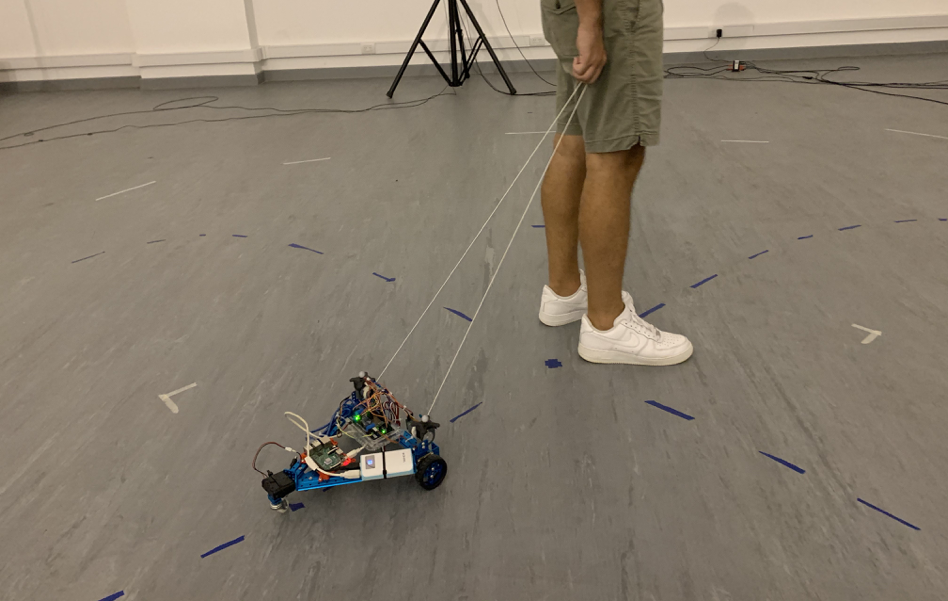
\includegraphics[width=8cm]{images/capture.png}
\caption{Hardware prototype on the motion capture system and a testing subject holding the threads.  On top of the device, two markers are placed and an additional marker is on a glove that the user is wearing (not shown on the picture).  The lemniscate of Gerono was marked on the floor.  The subject follows this track on the performed experiments.}
\label{fig:capturesystem}
\end{figure}



\section{Results} \label{Results}
\label{results}

Simulation results for both control strategies are shown on Figure~\ref{fig:simulationresults}. Subfigures (a) and (b) expound the trajectories of the leader and the follower for each strategy, while (c) and (d) describe their speed profiles.  Subfigure (e) show the distance between the robot and the patient for both strategies.  Results metrics for the simulations are shown on Table~\ref{tab:simulationmetricsftt} for the \textit{Follow the thread} strategy, whereas metrics for \textit{Rotate and go} are shown on Table~\ref{tab:simulationmetricsrg}.


\begin{center}
\begin{tabular}{ |c|c|c|c| }
\hline
$c_v$ & $c_{\alpha}$ & m.t.d. & t.t.d. \\
\hline
10  &   15  & 0.3614 & 2.0651\\
15  &   5  & 0.4325 & 2.055\\
\textbf{15}  &   \textbf{10}  & \textbf{0.2188} & \textbf{1.0902}\\
15  &   15  & 0.2891 & 1.5059\\
5  &   20  & 0.5733 & 3.7289\\
\hline
\end{tabular}
\captionof{table}{Maximum trajectory deviation m.t.d. (m) and Total trajectory deviation t.t.d. for different \textit{Follow the thread} constants.}
\label{tab:simulationmetricsftt}
\end{center}


\begin{center}
\begin{tabular}{ |c|c|c|c|c| }
\hline
$c_v$ & $c_r$ & $Dt_{off}$ & m.t.d. & t.t.d.\\
\hline
10  &   20  &   0.1  & 0.4310 & 1.6380\\
20  &   20  &   0.05  & 0.7775 & 3.1139\\
\textbf{20}  &  \textbf{20}  & \textbf{0.1} & \textbf{0.4123} & \textbf{0.9872}\\
20  &   35  &   0.1  & 0.4143 & 1.4820\\
20  &   5  &  0.05  & 0.7815 & 3.0892\\
35  &   20  &   0.1  & 0.6337 & 1.6190\\
\hline
\end{tabular}
\captionof{table}{Maximum trajectory deviation m.t.d. (m) and total trajectory deviation t.t.d. for different \textit{Rotate and go} constants.}
\label{tab:simulationmetricsrg}
\end{center}

%\begin{figure}[h!]
%\centering
%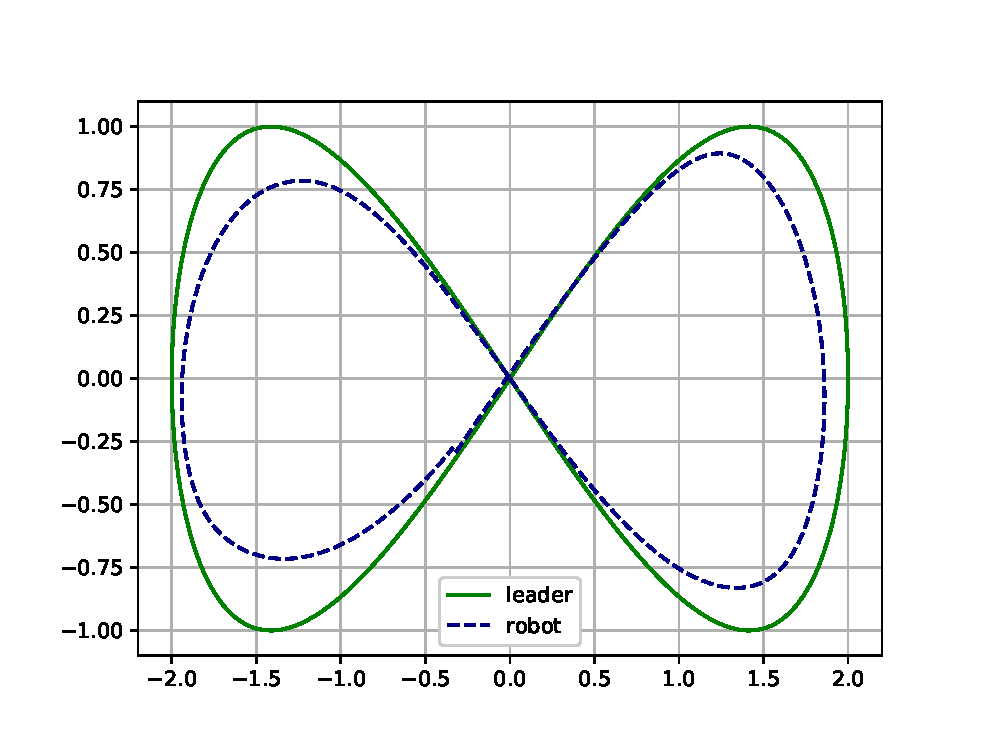
\includegraphics[width=8cm]{images/ft_a2_n1500_cv15_cr15.eps}
%\caption{Trajectories of the leader and follower for the \textit{Follow the thread} control strategy.}
%\label{fig:distance_sim}
%\end{figure}
%
%\begin{figure}[h!]
%\centering
%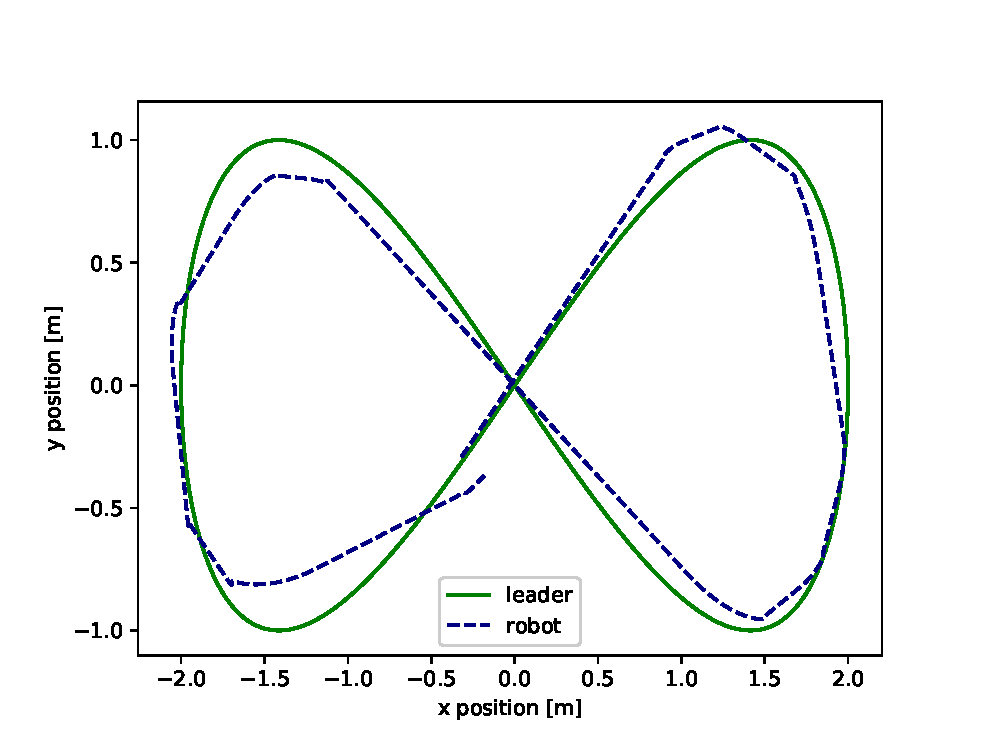
\includegraphics[width=8cm]{images/rgv_cv20_cr20_dr10.eps}
%\caption{Trajectories of the leader and follower for \textit{Rotate and go} control strategy.}
%\label{fig:distance_sim}
%\end{figure}
%
%\begin{figure}[h!]
%\centering
%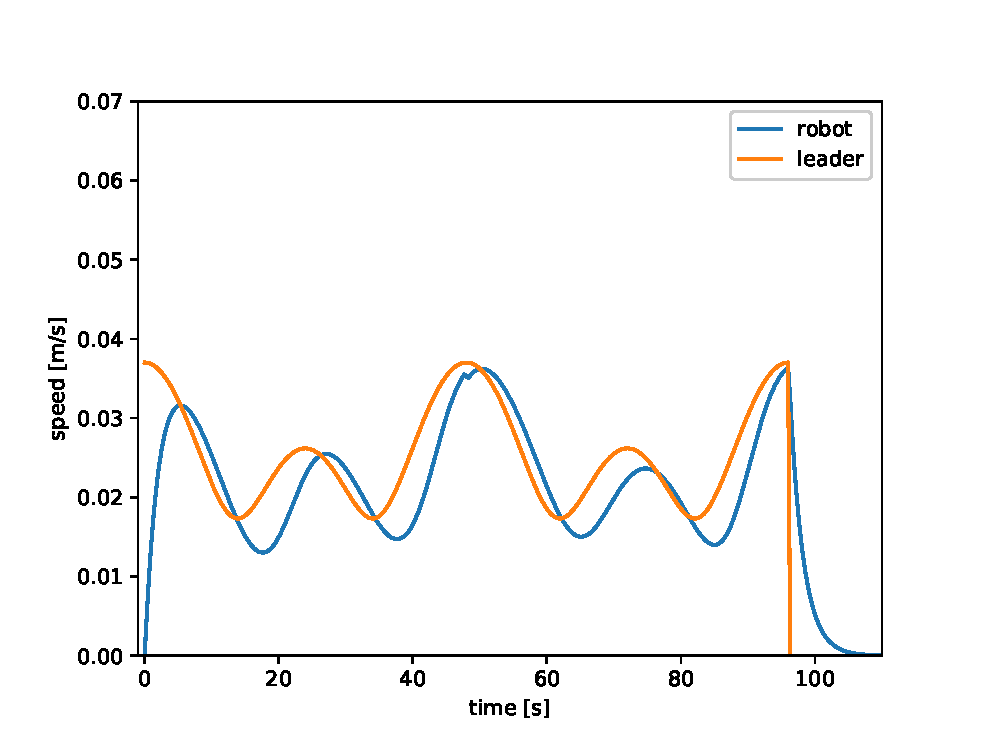
\includegraphics[width=8cm]{images/ft_cv15_cr10_leader_robot_speed.eps}
%\caption{Speed profiles of the leader and follower for \textit{Follow the thread} control strategy.}
%\label{fig:distance_sim}
%\end{figure}
%
%\begin{figure}[h!]
%\centering
%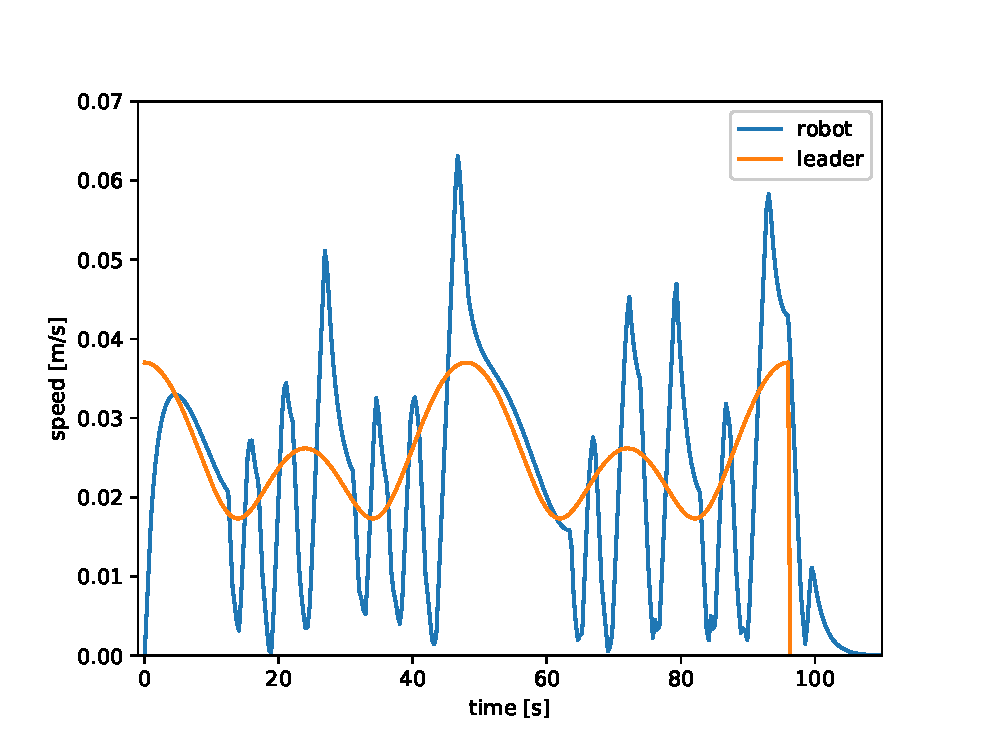
\includegraphics[width=8cm]{images/rg_cv20_cr20_bv10_dtoff10_leader_robot_speed.eps}
%\caption{Speed profiles of the leader and follower for \textit{Rotate and go} control strategy.}
%\label{fig:distance_sim}
%\end{figure}
%
%\begin{figure}[h!]
%\centering
%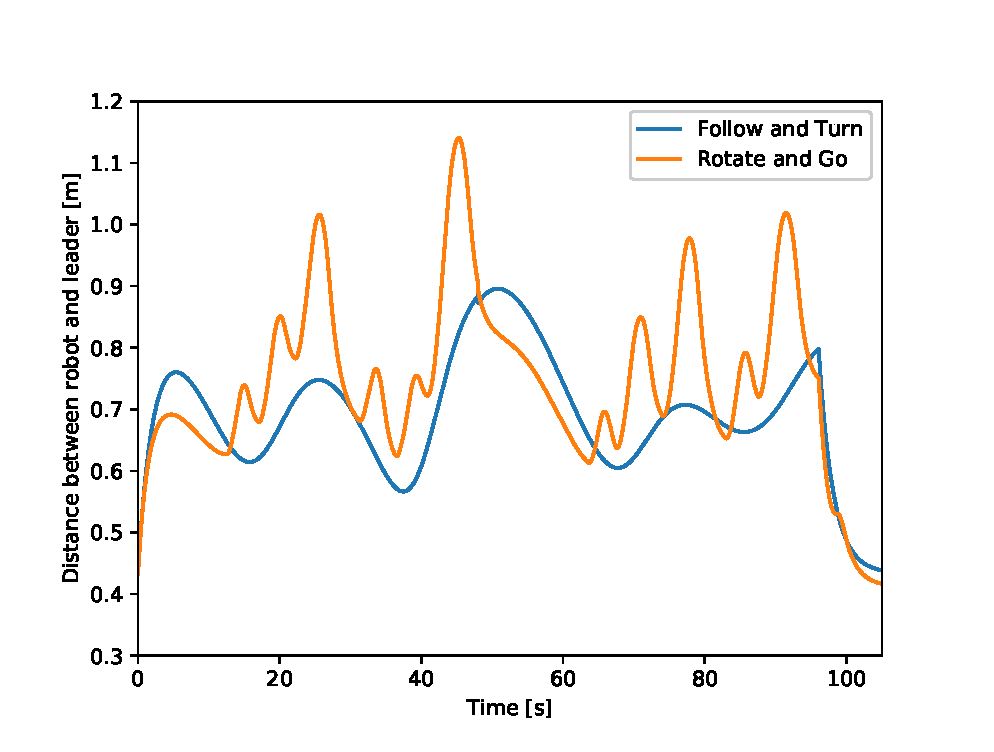
\includegraphics[width=8cm]{images/ft_vs_rg_dist.eps}
%\caption{Separation distance between robot and leader for both strategies [m].}
%\label{fig:distance_sim}
%\end{figure}


\begin{figure} 
    \centering
  \subfloat[ \label{sr1a}]{%
       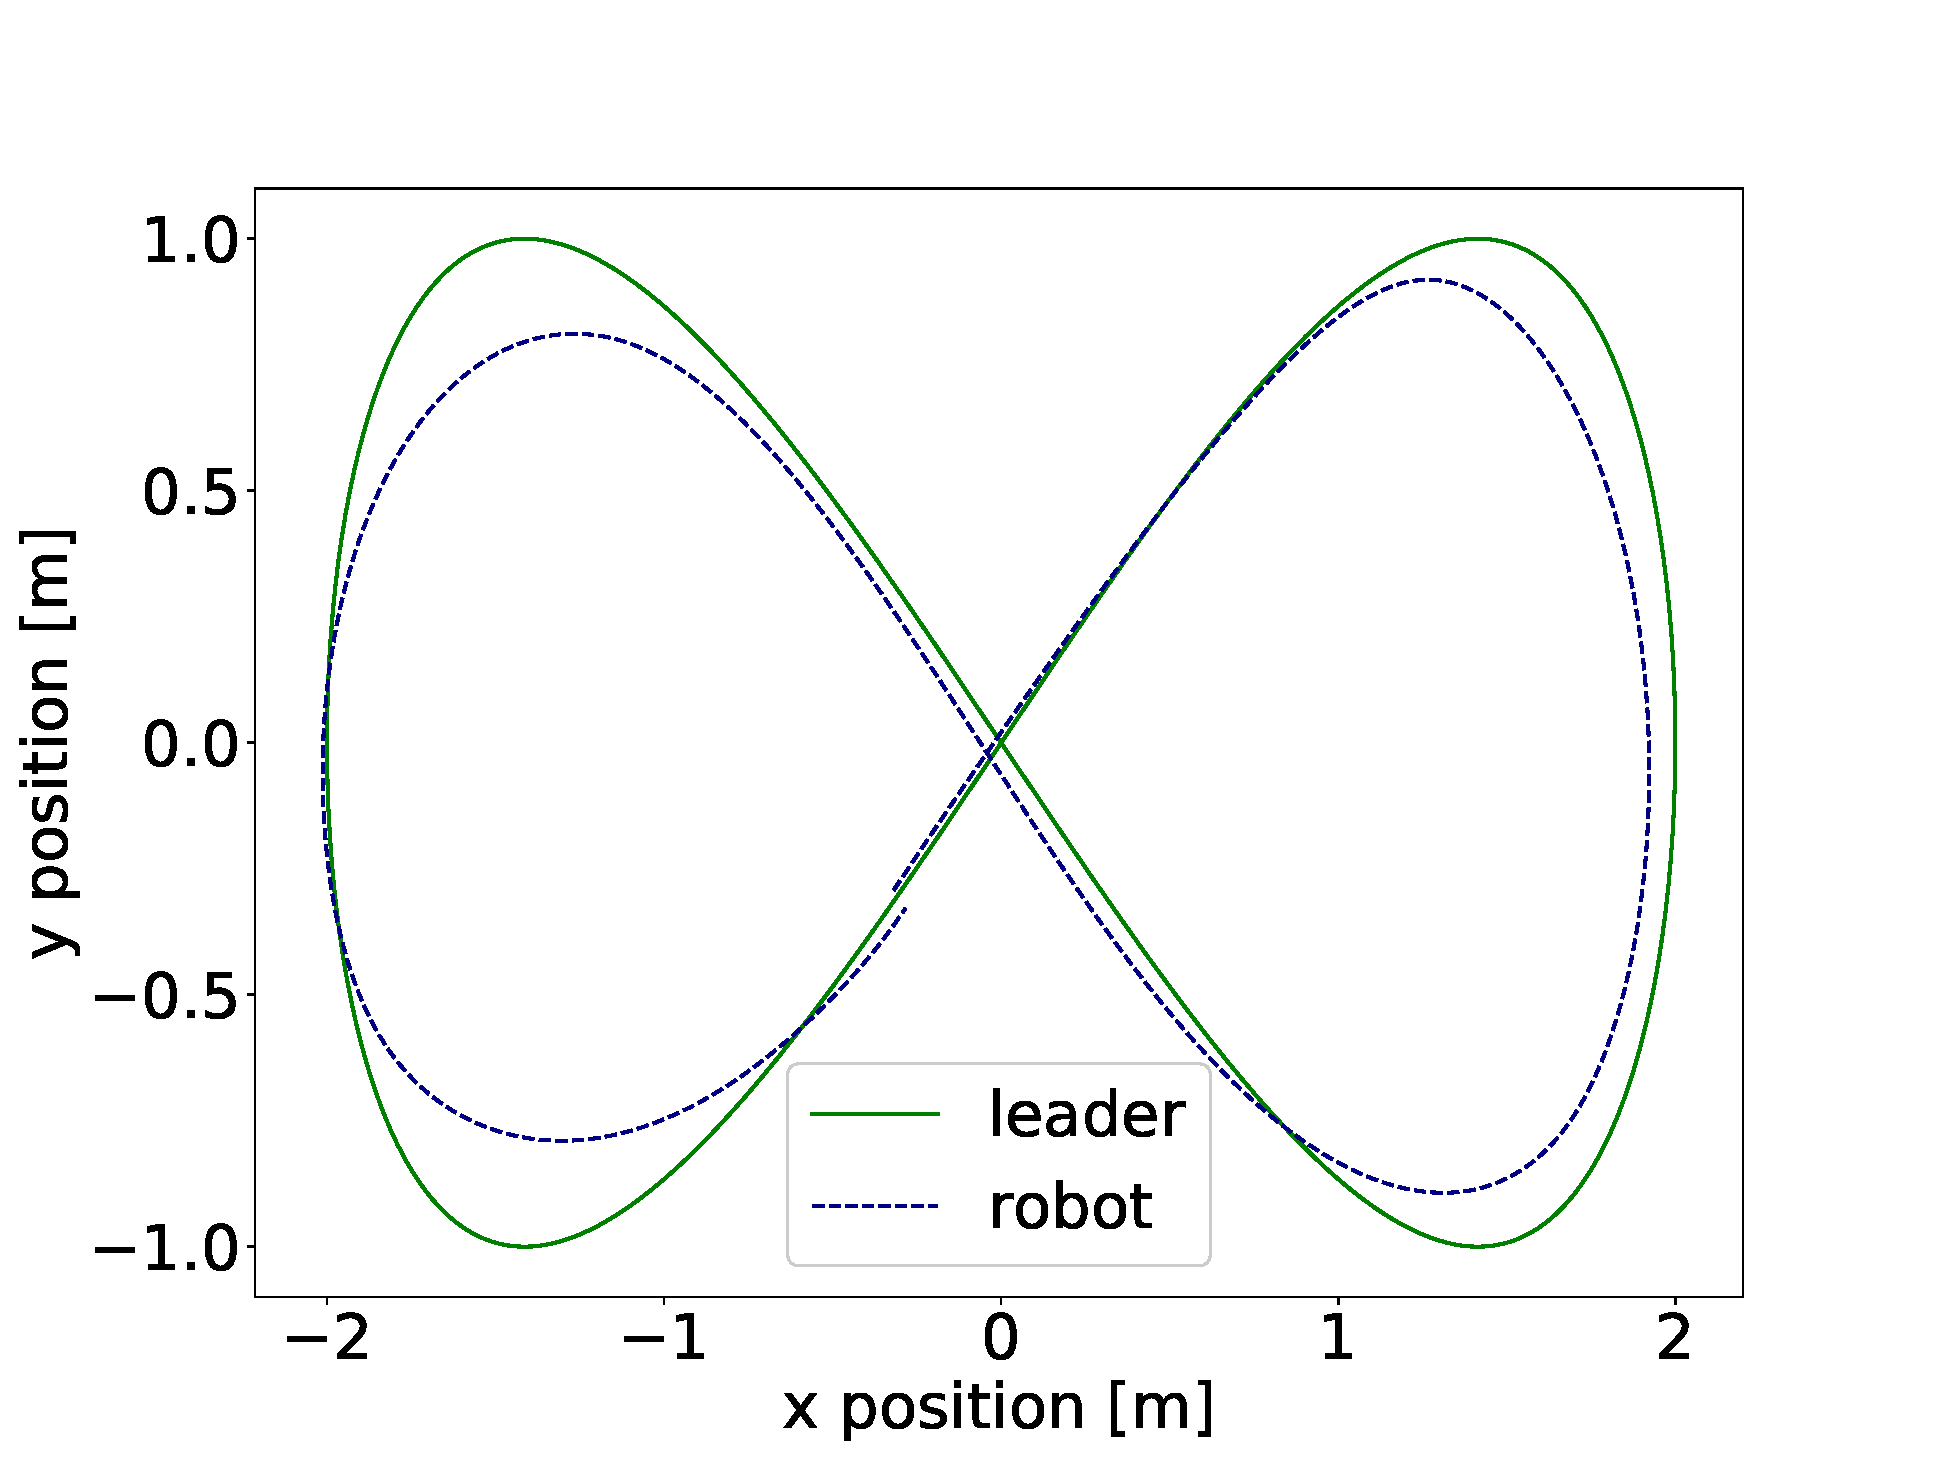
\includegraphics[width=0.49\linewidth]{images/simulation_follow-thread.eps}}
    \hspace*{-1.5em}
  \subfloat[ \label{sr1b}]{%
        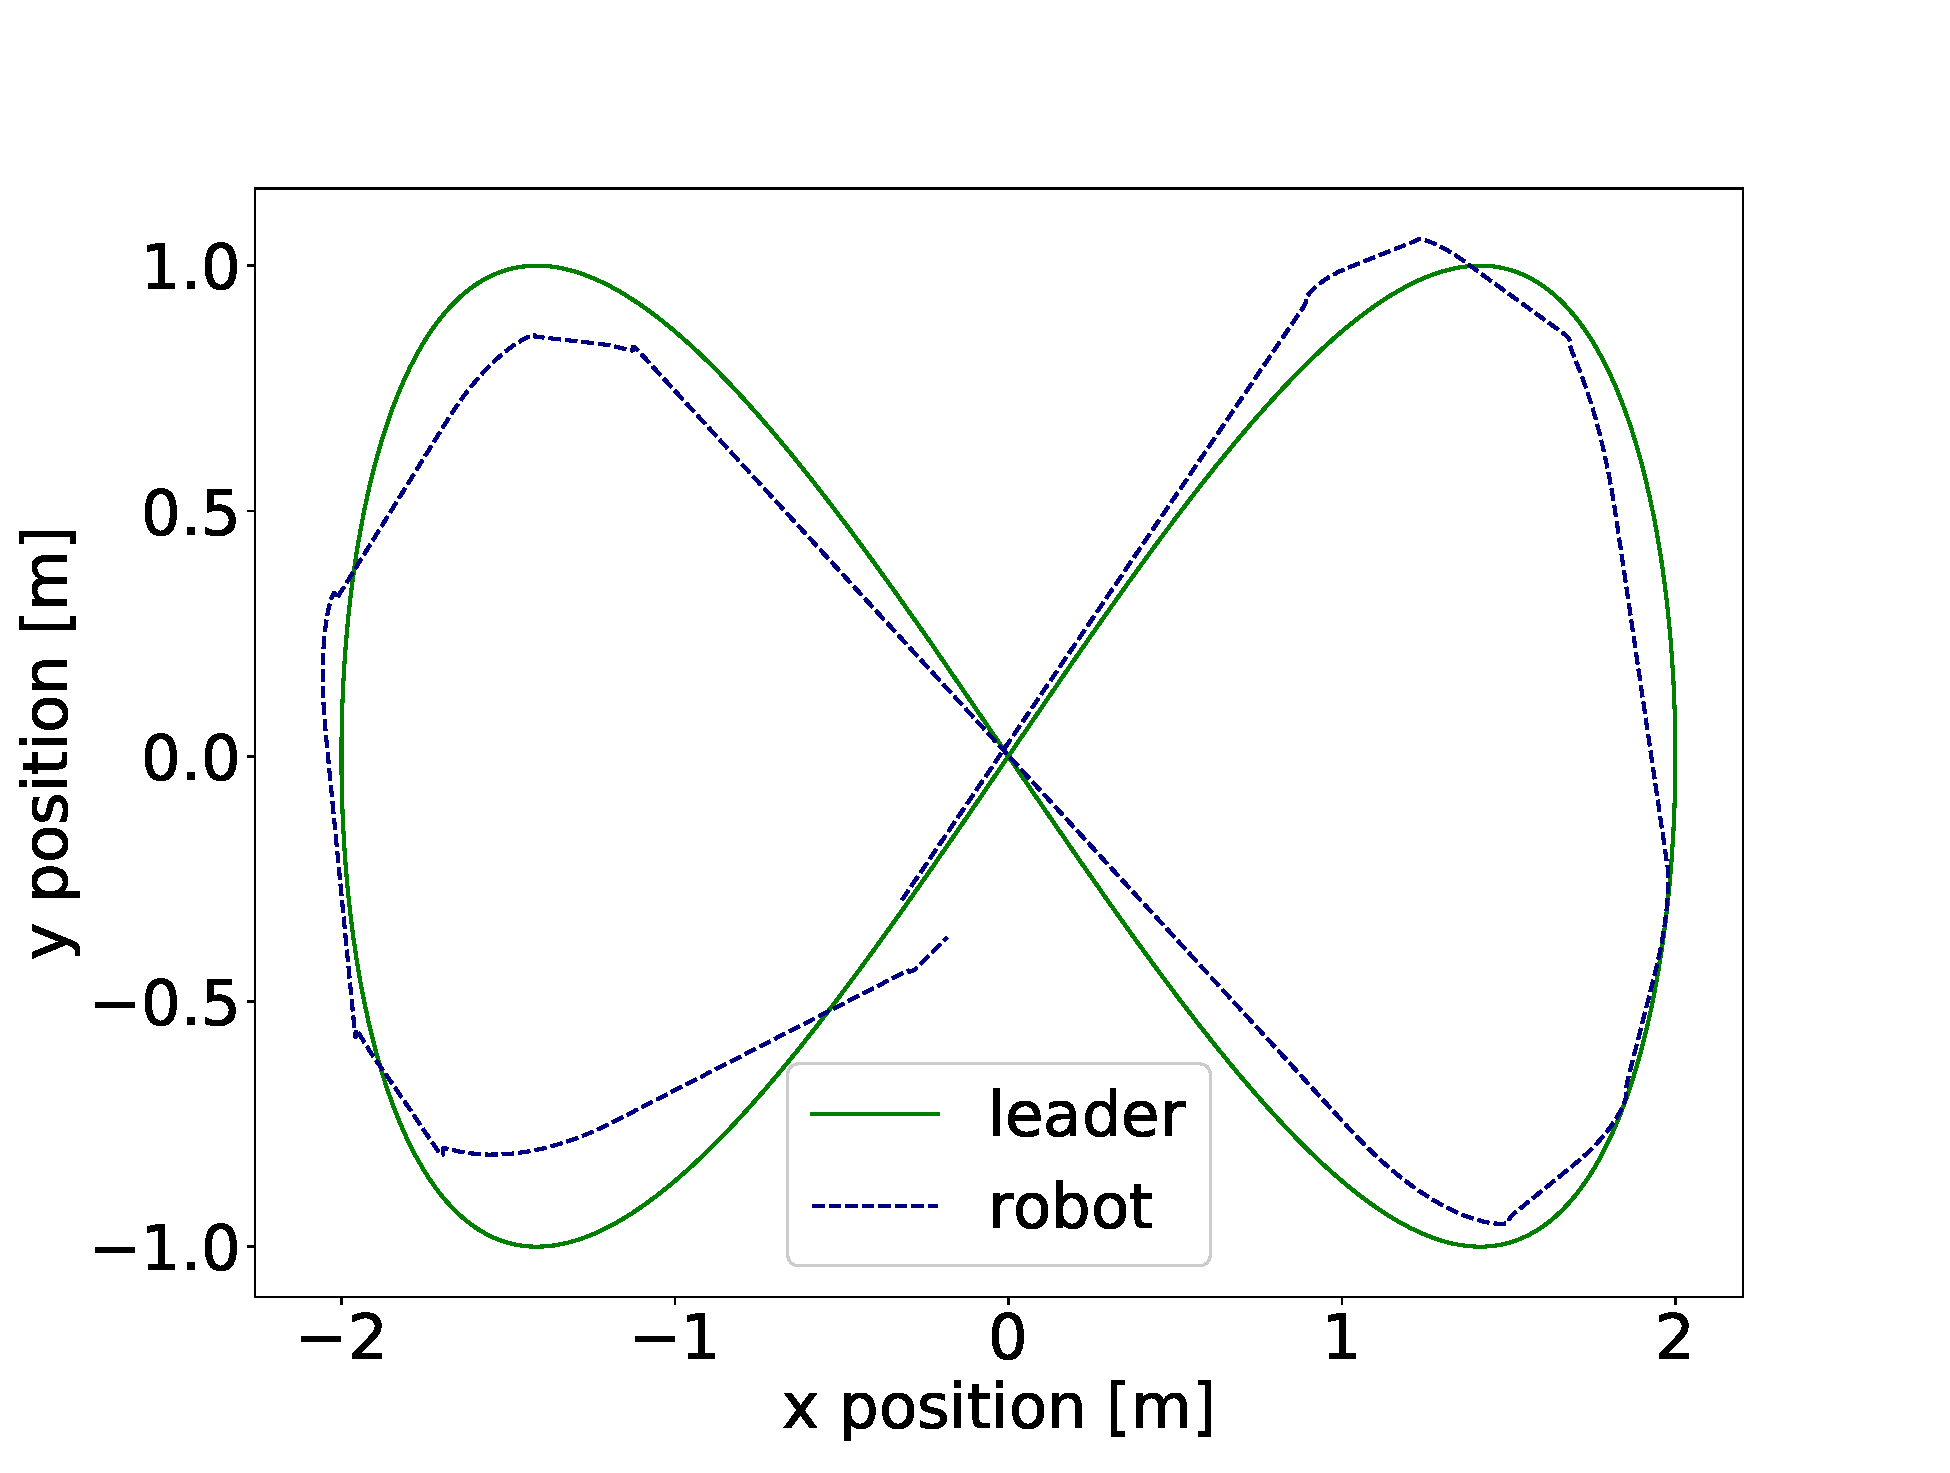
\includegraphics[width=0.49\linewidth]{images/simulation_rotate-go.eps}}
    \\
    \vspace*{-1.1em}
  \subfloat[ \label{sr1c}]{%
        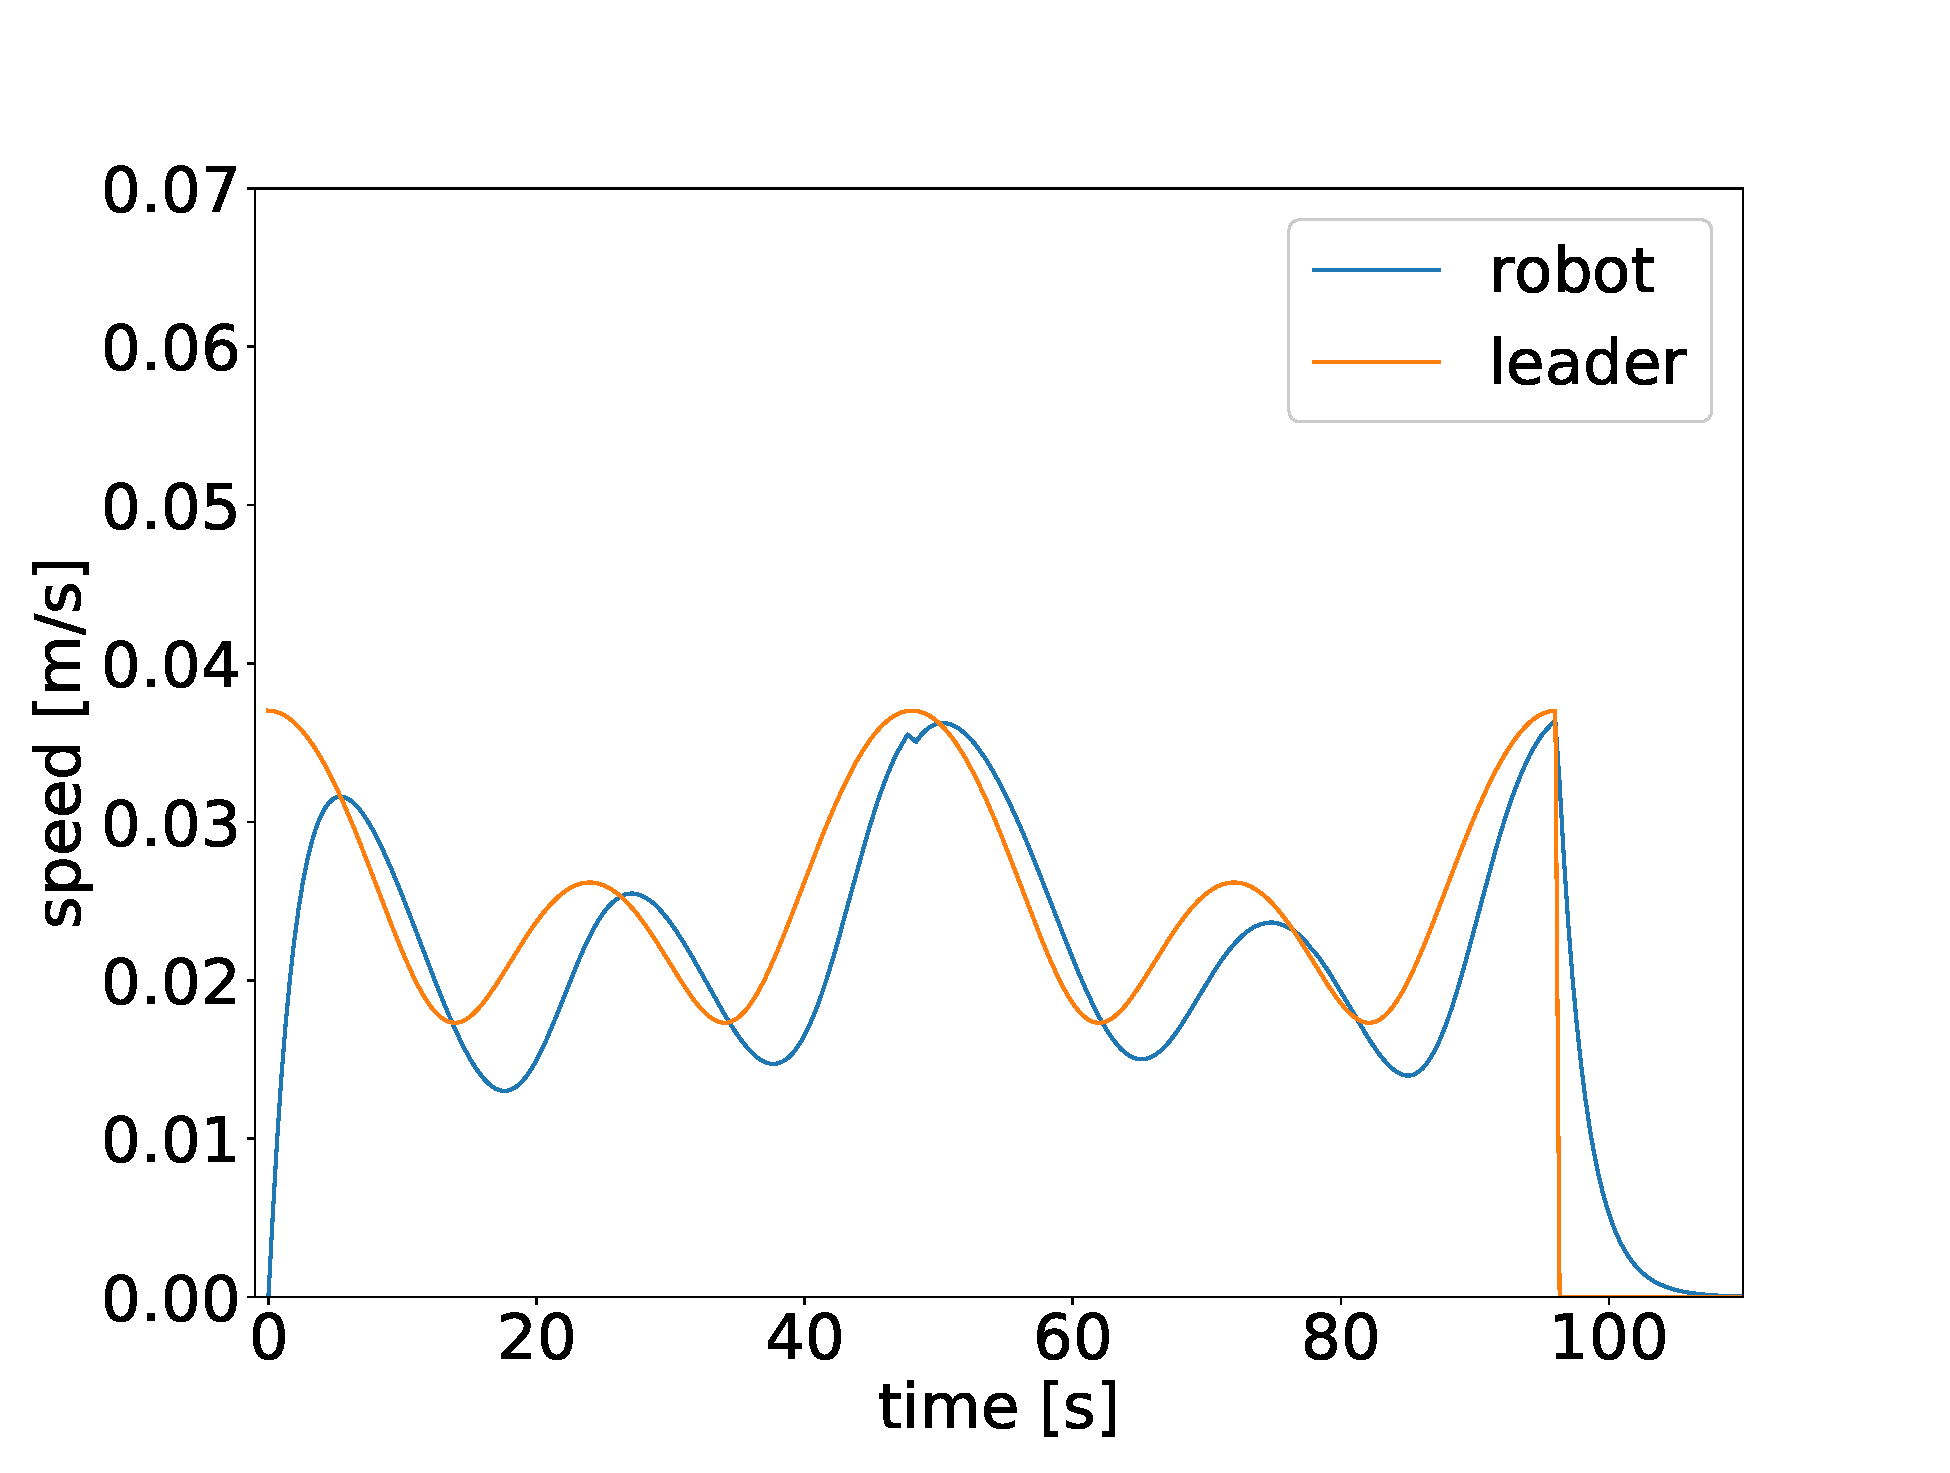
\includegraphics[width=0.49\linewidth]{images/simulation_speed_profile_follow-thread.eps}}
    \hspace*{-1.5em}
  \subfloat[ \label{sr1d}]{%
        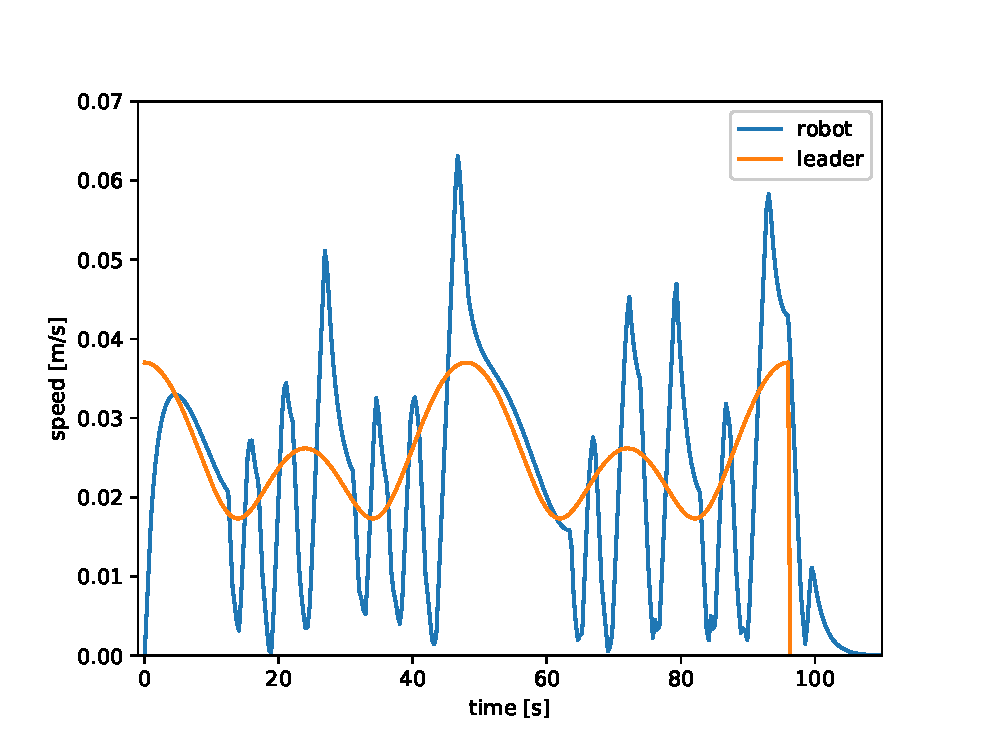
\includegraphics[width=0.49\linewidth]{images/simulation_speed_profile_rotate-go.eps}}
    \\
    \vspace*{-2.5em}
  \subfloat[ \label{sr1e}]{%
        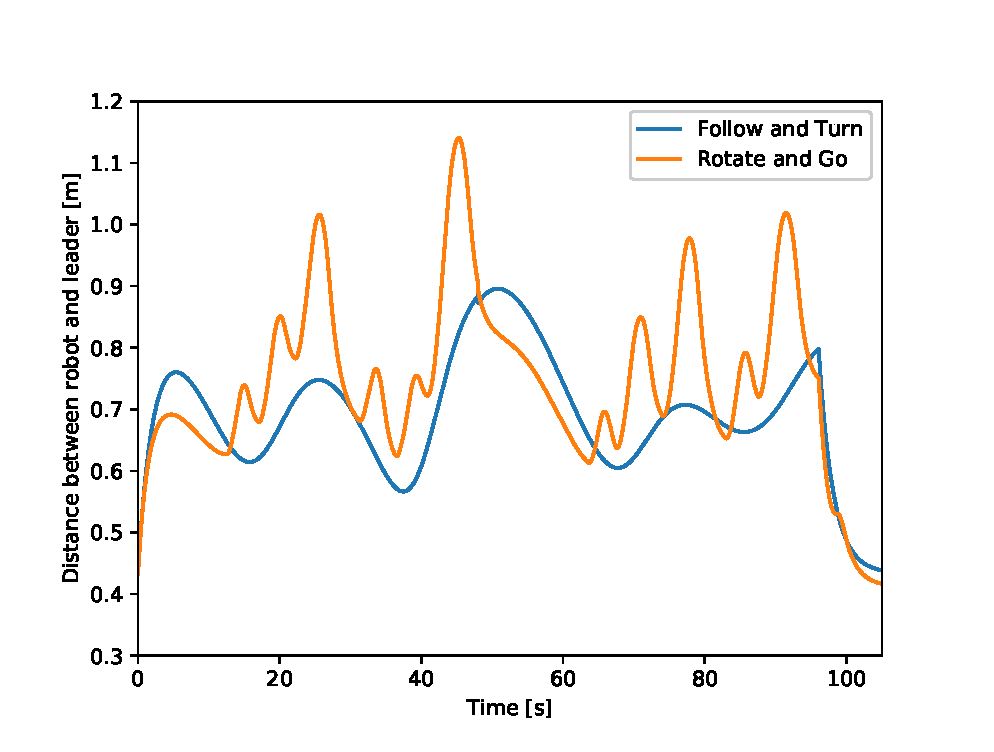
\includegraphics[width=0.99\linewidth]{images/ft_vs_rg_dist.eps}}
  \caption{Simulation Results: Trajectories of the leader and follower for \textit{Follow the thread} (a) and \textit{Rotate and go} (b) . 
        Speed profiles of the leader and follower for \textit{Follow the thread} (c) and \textit{Rotate and go} (d). 
        (e) Separation distance between robot and leader for both strategies  (m).}
  \label{fig:simulationresults} 
\end{figure}



Results for the real world experiment can be seen on Figure~\ref{fig:realworldresults}.   Table~\ref{tab:cap_ft_npd_table} shows the metrics of the \textit{Follow the thread} strategy, whereas Table~\ref{tab:cap_rg_npd_table} provides the metrics for the \textit{Rotate and go} approach.

%\begin{figure}[h!]
%\centering
%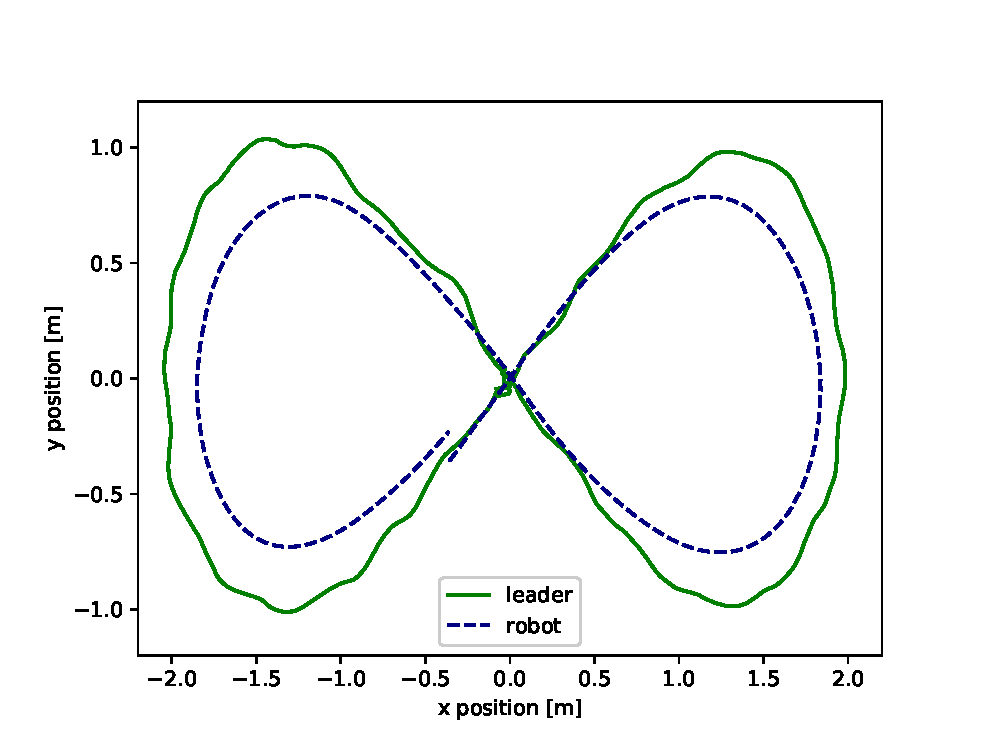
\includegraphics[width=8cm]{images/ft1cap.eps}
%\caption{Trajectories for the \textit{Follow the thread} control strategy.}
%\label{fig:distance_sim}
%\end{figure}
%
%
%\begin{figure}[h!]
%\centering
%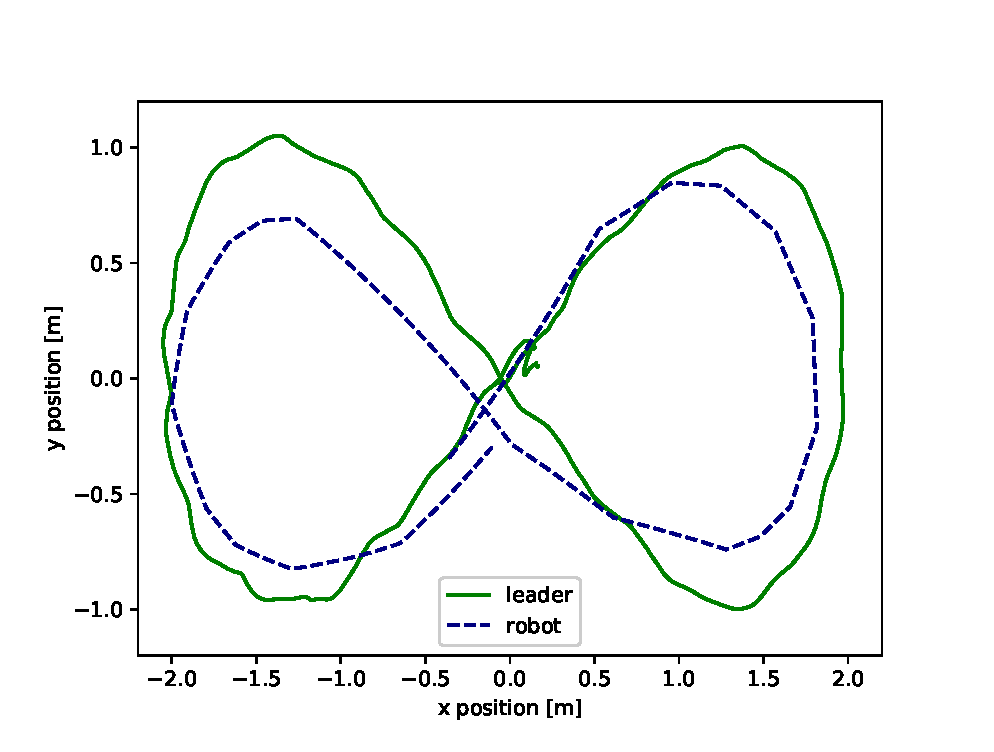
\includegraphics[width=8cm]{images/rg2cap.eps}
%\caption{Distance between robot and leader [m]}
%\label{fig:distance_sim}
%\end{figure}
%
%
%\begin{figure}[h!]
%\centering
%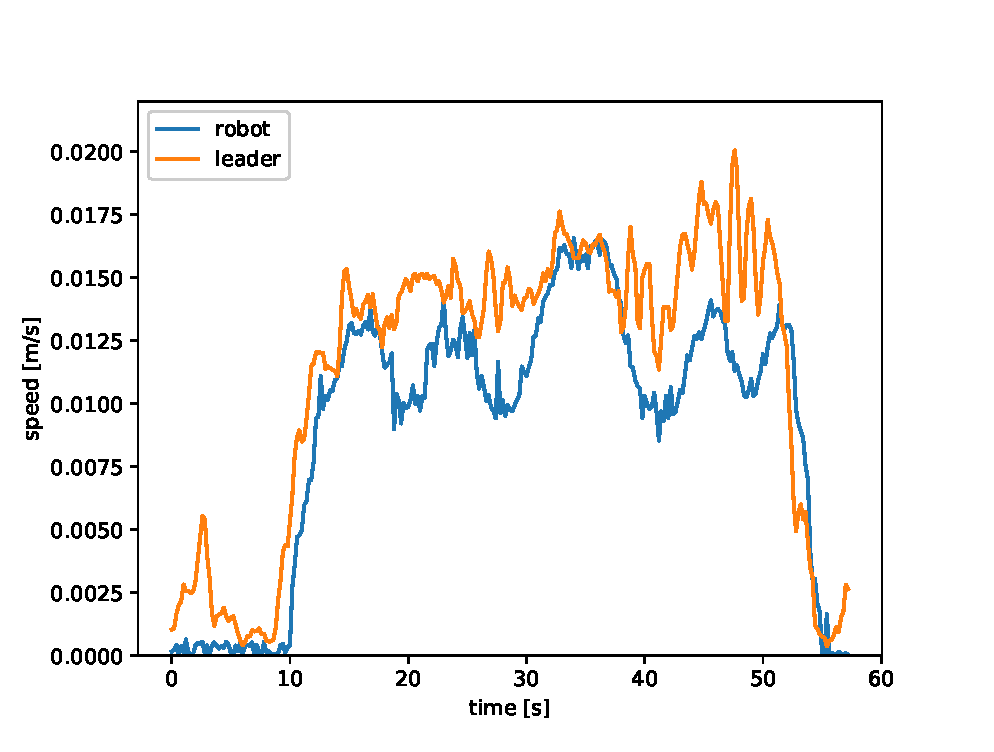
\includegraphics[width=8cm]{images/ft1cap_leader_robot_speed.eps}
%\caption{\textit{Follow the thread} speed profiles}
%\label{fig:distance_sim}
%\end{figure}
%
%
%\begin{figure}[h!]
%\centering
%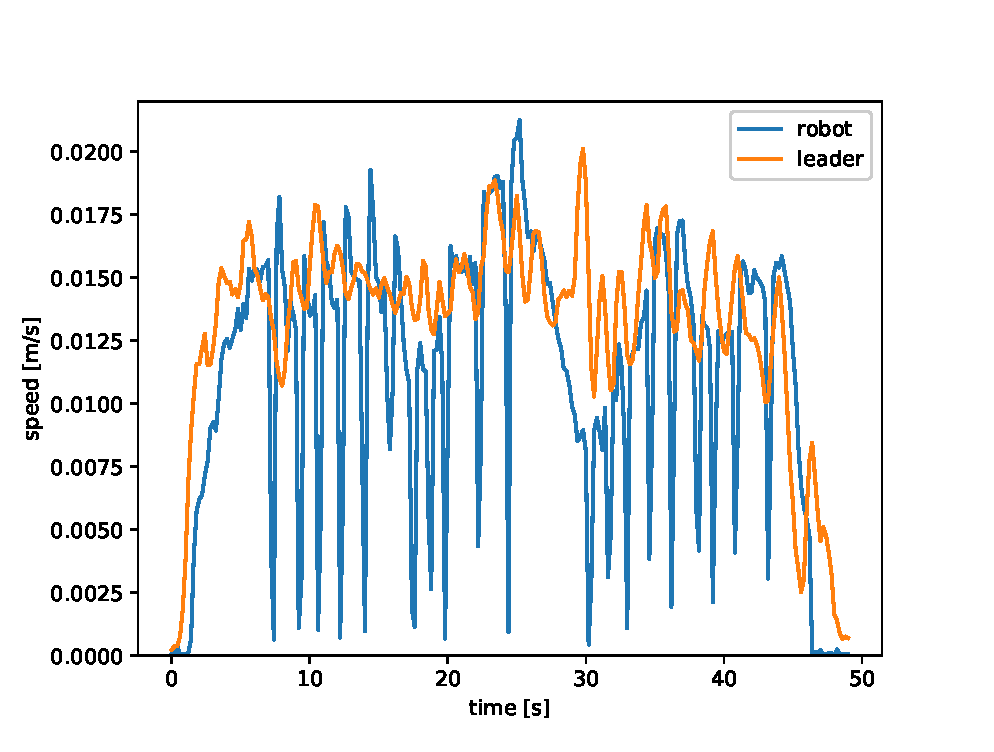
\includegraphics[width=8cm]{images/rg2cap_leader_robot_speed.eps}
%\caption{Rotate and go speed profiles}
%\label{fig:distance_sim}
%\end{figure}
%
%
%\begin{figure}[h!]
%\centering
%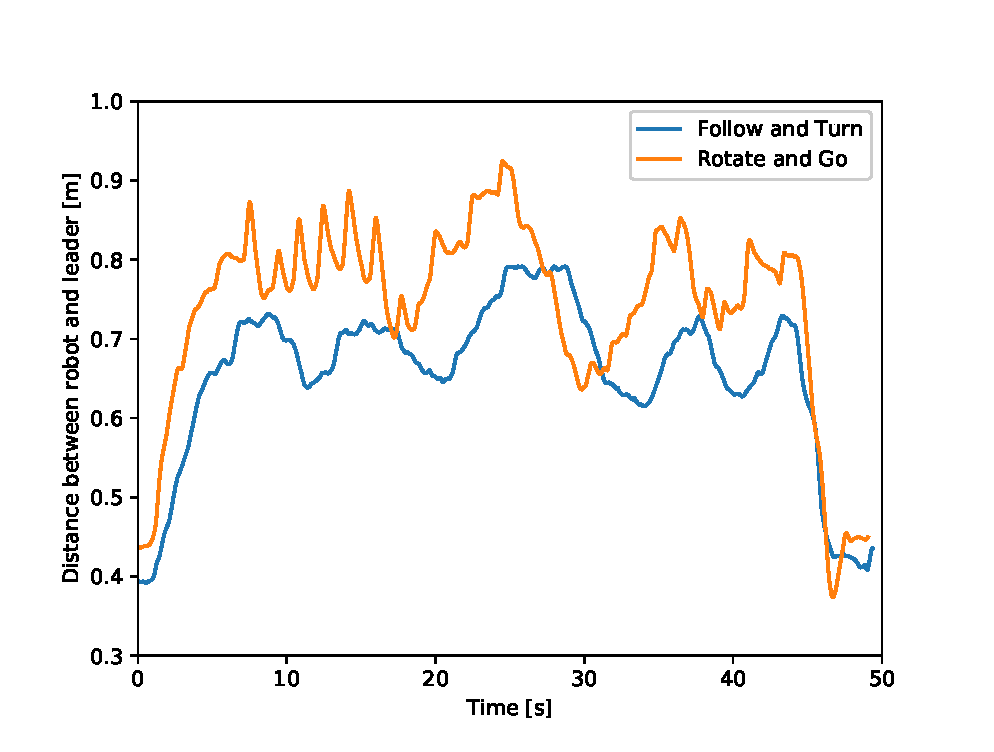
\includegraphics[width=8cm]{images/cap_ft_vs_rg_dist.eps}
%\caption{\textit{Rotate and go} speed profiles}
%\label{fig:distance_sim}
%\end{figure}


\begin{figure} 
    \centering
  \subfloat[ \label{rw1a}]{%
       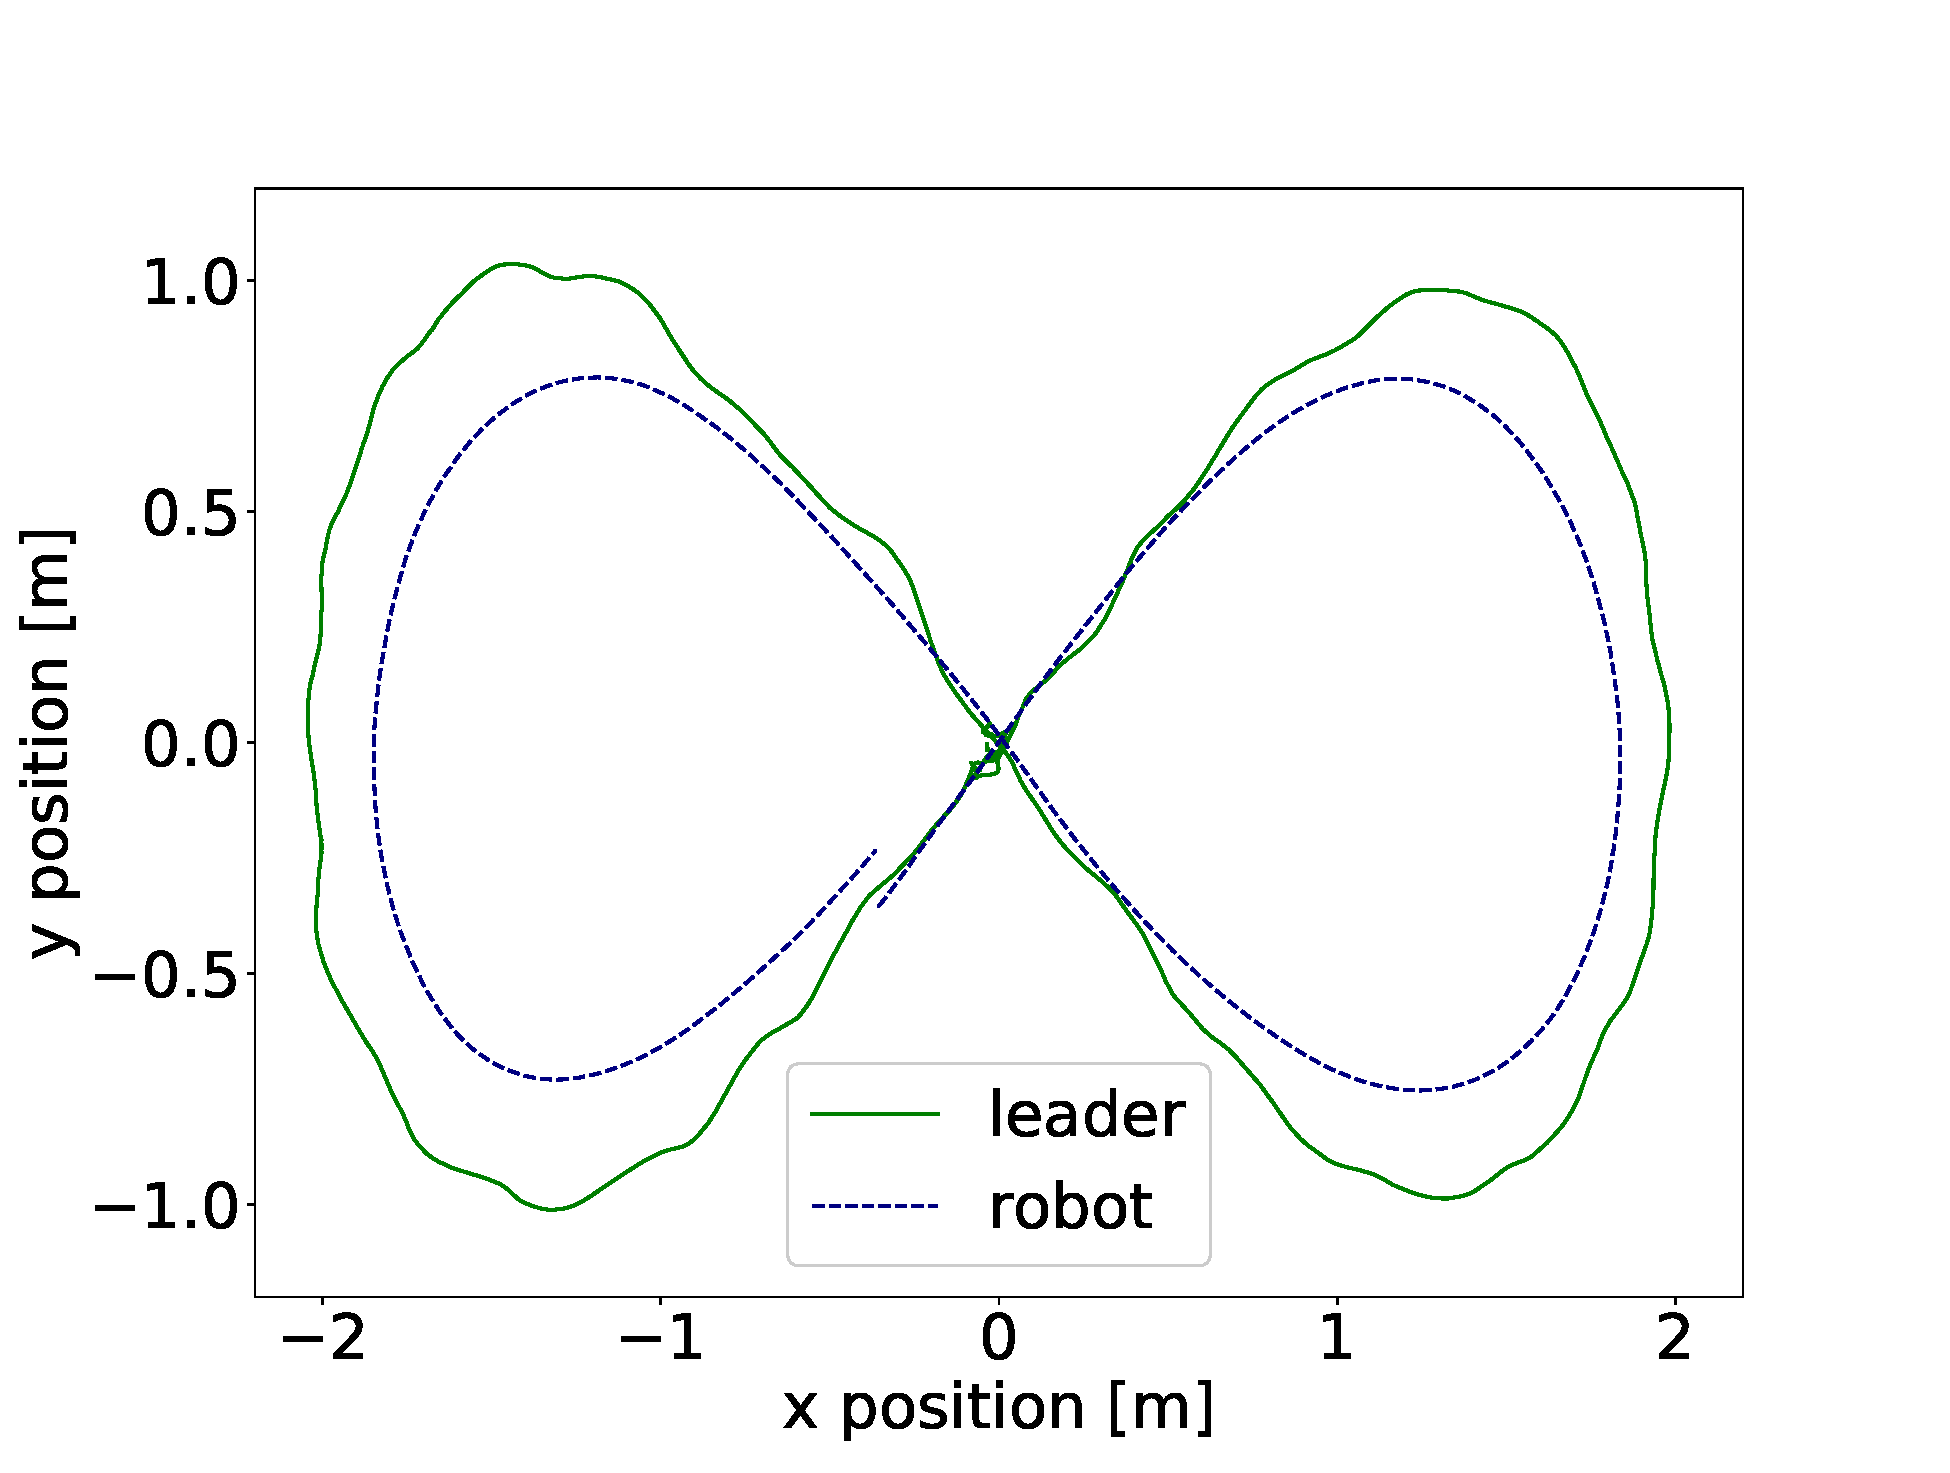
\includegraphics[width=0.49\linewidth]{images/capture_follow-turn.eps}}
    \hspace*{-1.5em}
  \subfloat[ \label{rw1b}]{%
        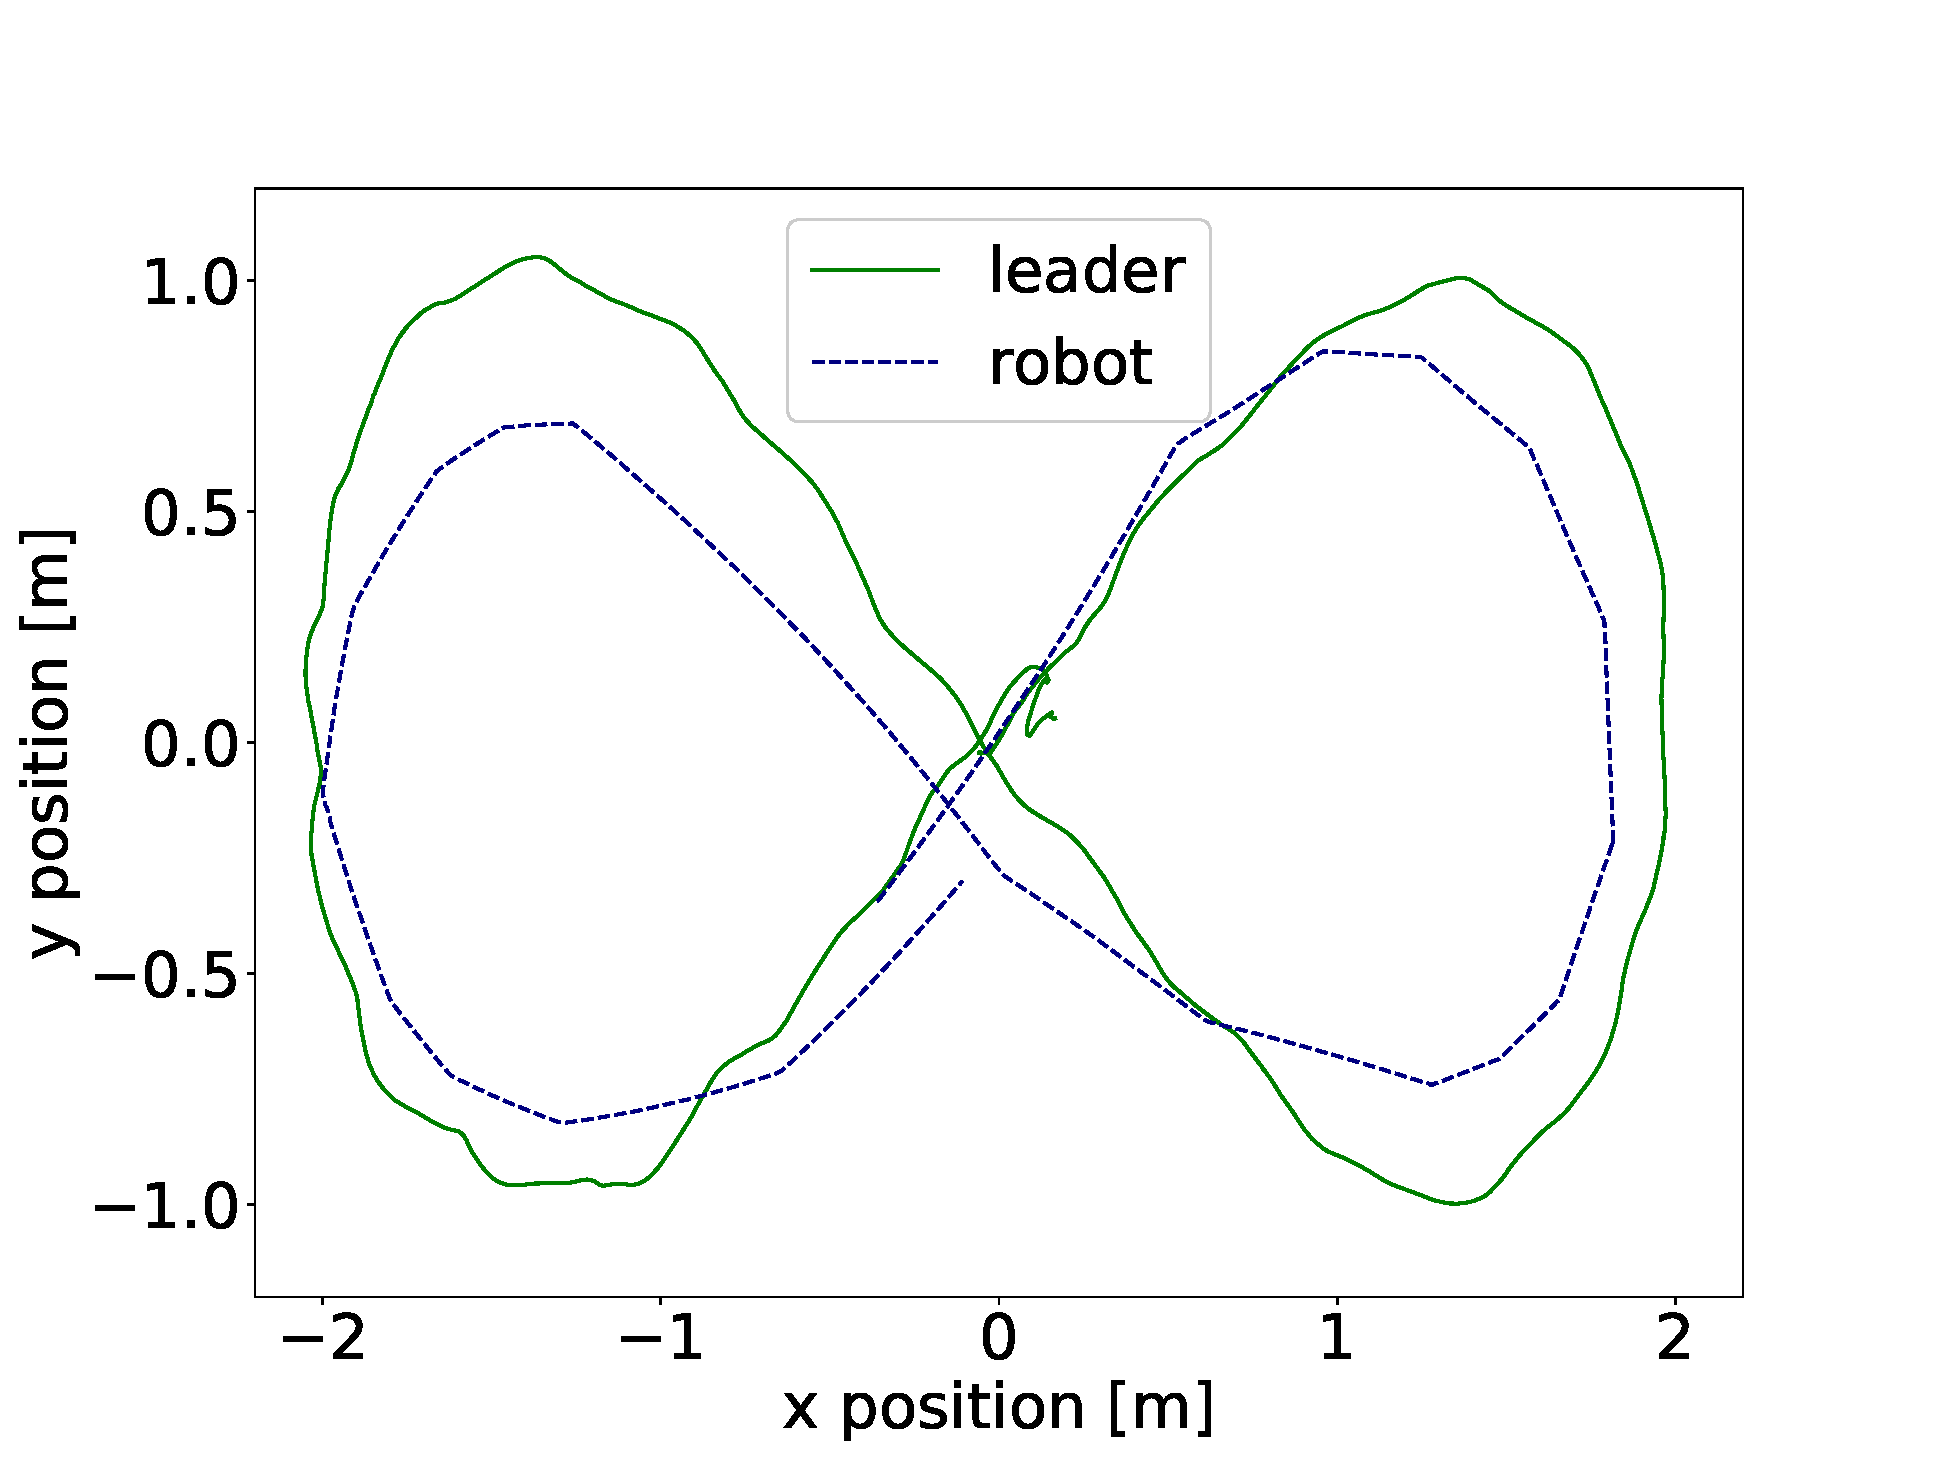
\includegraphics[width=0.49\linewidth]{images/capture_rotate-go.eps}}
    \\
    \vspace*{-1.1em}
  \subfloat[ \label{rw1c}]{%
        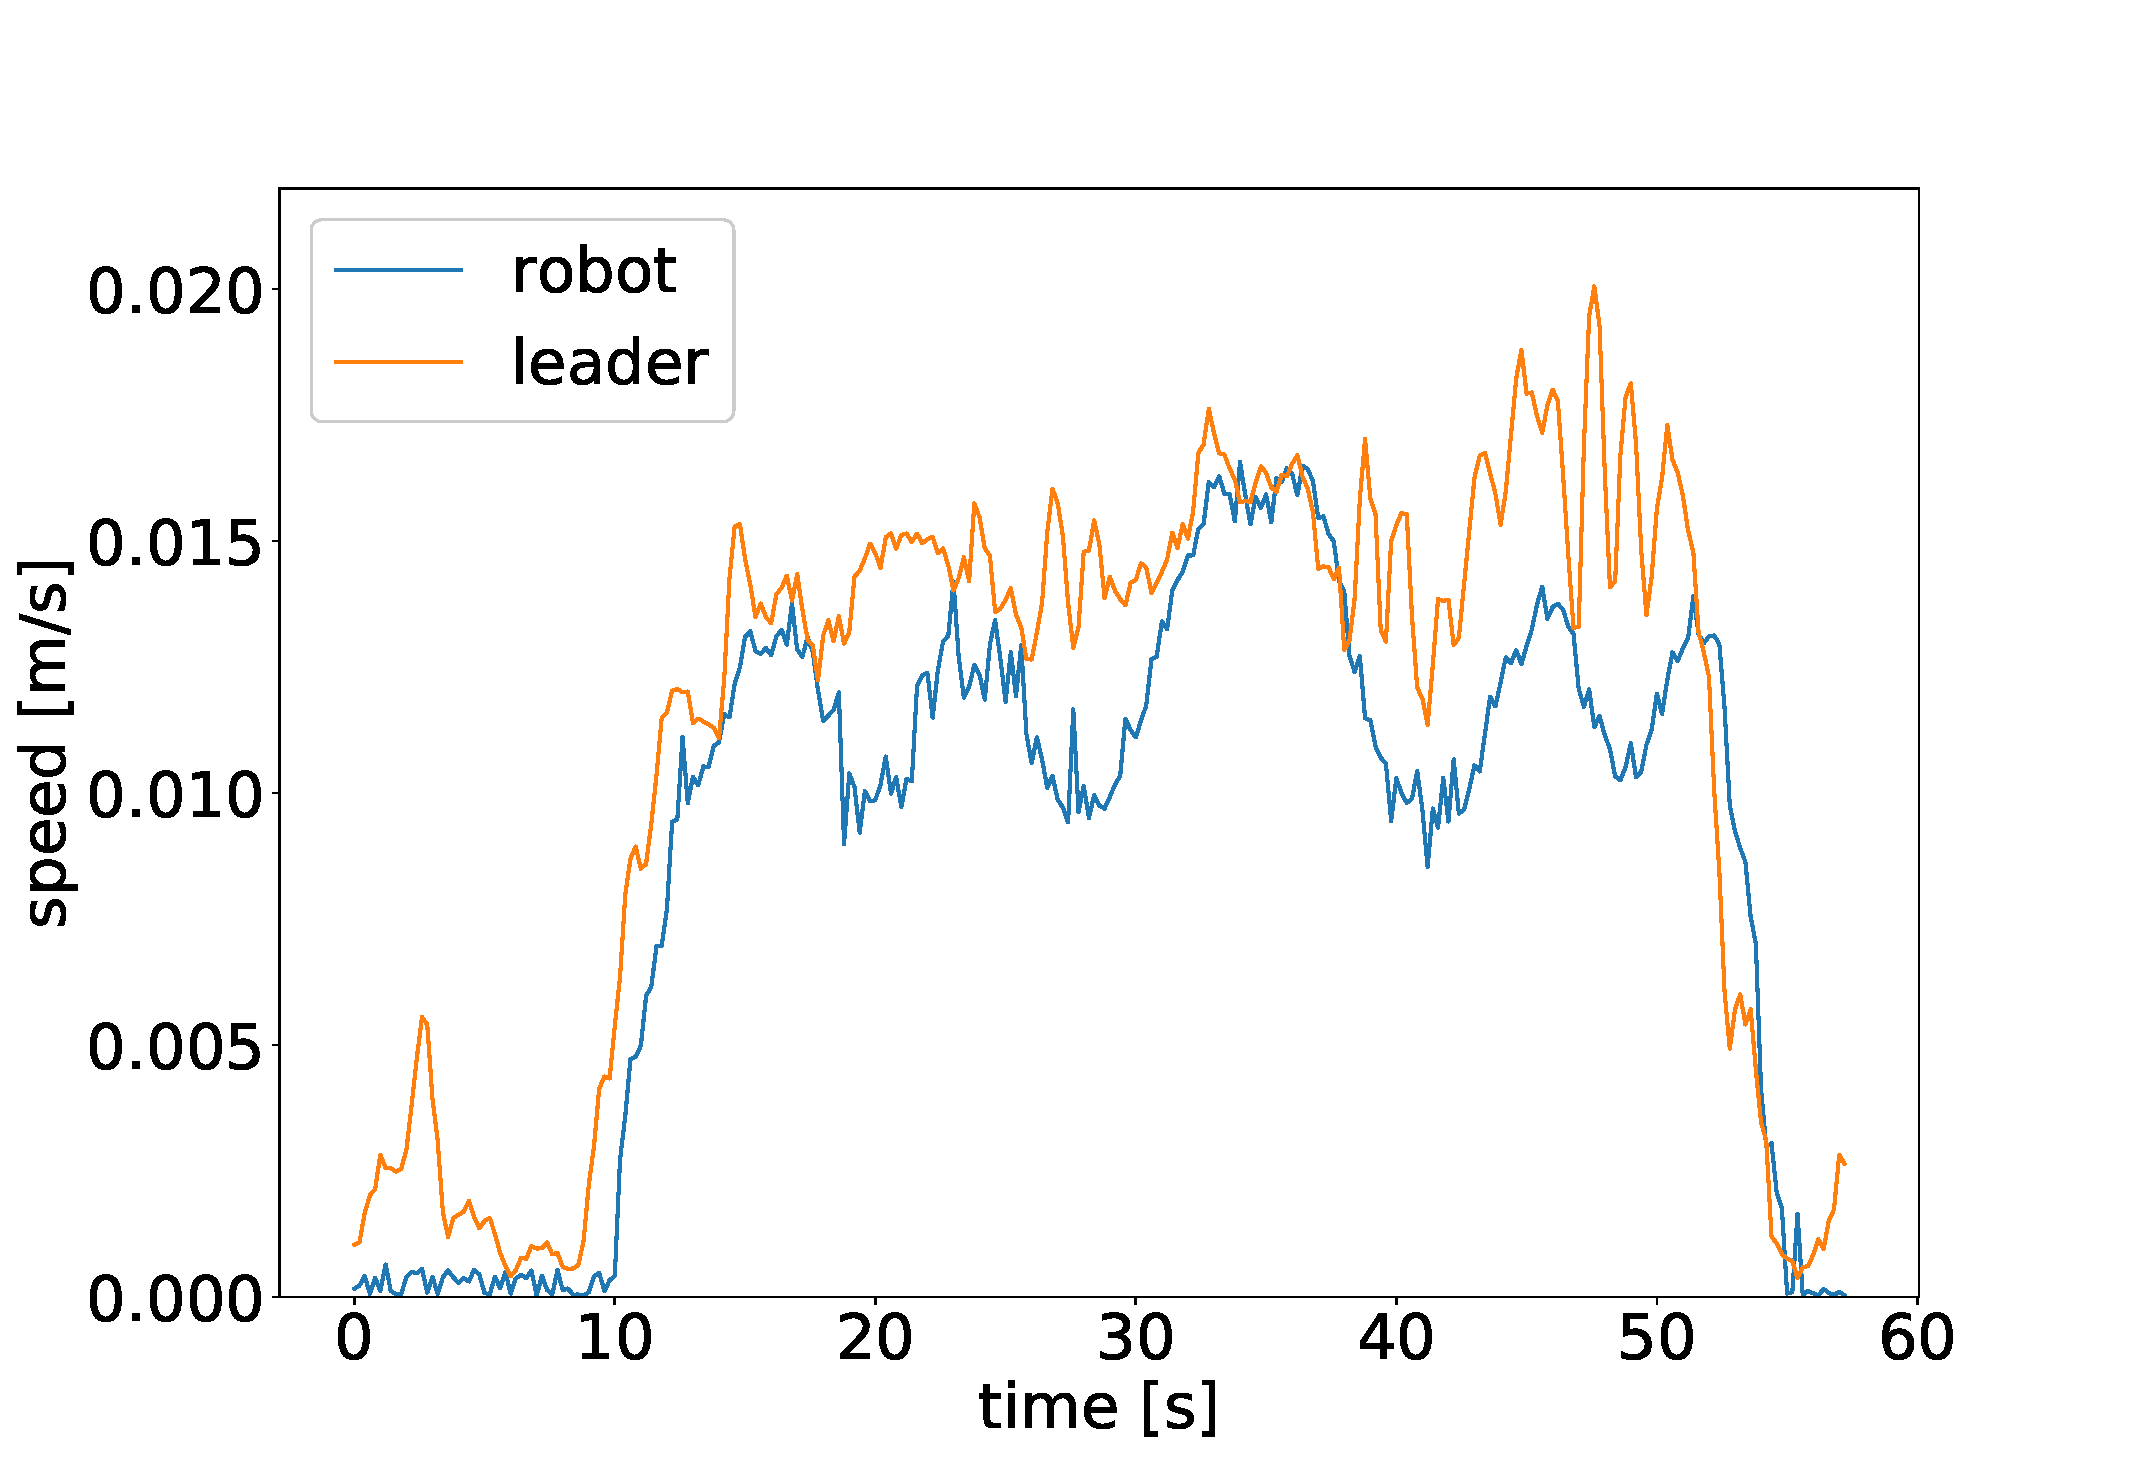
\includegraphics[width=0.49\linewidth]{images/capture_speed_profile_follow-thread.eps}}
    \hspace*{-1.5em}
  \subfloat[ \label{rw1d}]{%
        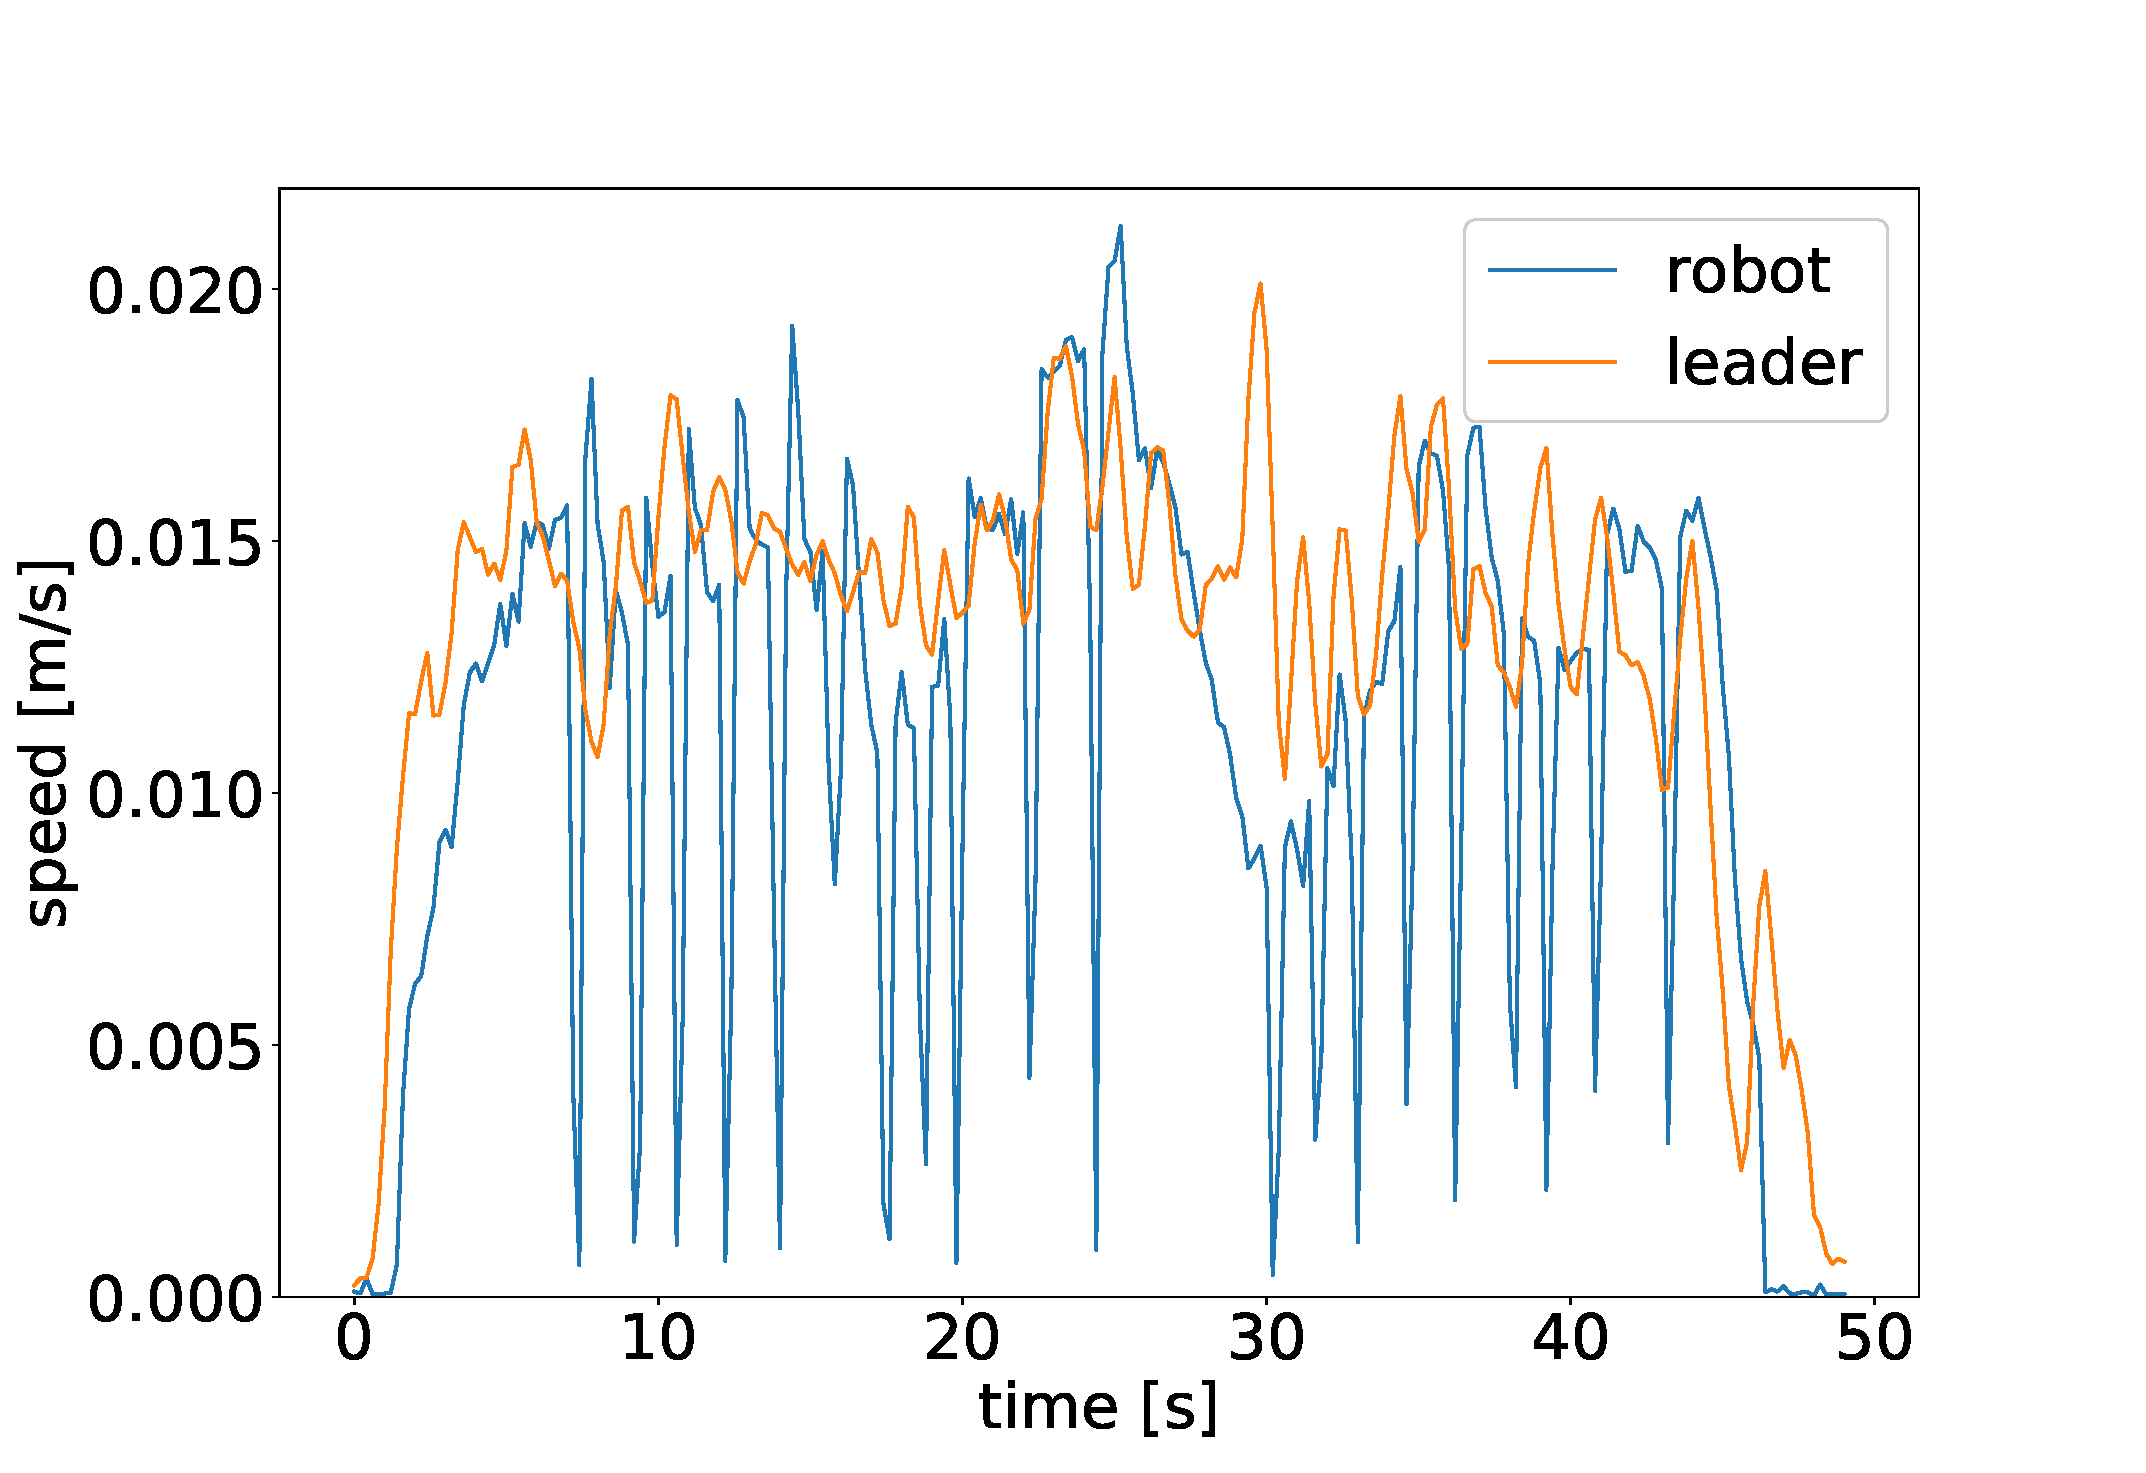
\includegraphics[width=0.49\linewidth]{images/capture_speed_profile_rotate-go.eps}}
    \\
    \vspace*{-1.8em}
  \subfloat[ \label{rw1e}]{%
        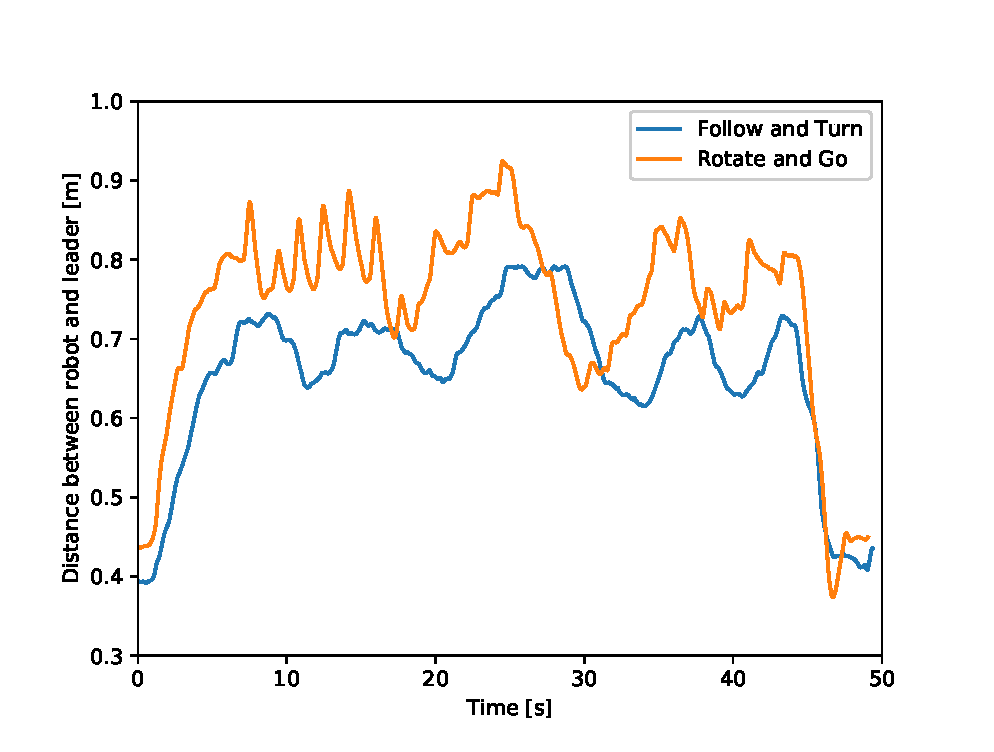
\includegraphics[width=0.99\linewidth]{images/cap_ft_vs_rg_dist.eps}}
  \caption{Experimentation Results: Trajectories of the leader and follower for \textit{Follow the thread} (a) and \textit{Rotate and go} (b). 
        Speed profiles of the leader and follower for \textit{Follow the thread} (c) and \textit{Rotate and go} (d). 
        (e) Separation distance between robot and leader for both strategies (m).}
  \label{fig:realworldresults} 
\end{figure}


\begin{center}
\begin{tabular}{ |c|c|c|c| }
\hline
$c_v$ & $c_{\alpha}$ & m.t.d. (m) & t.t.d. \\
\hline
\textbf{25}  &   \textbf{20}  & \textbf{0.3876} & \textbf{1.9761}\\
25  &   35  & 0.4672 & 2.3528\\
\hline
\end{tabular}
\captionof{table}{Maximum trajectory deviation m.t.d. and area under normal trajectory deviation t.t.d. in motion capture experiments using \textit{Follow the thread}.}
\label{tab:cap_ft_npd_table}
\end{center}


\begin{center}
\begin{tabular}{ |c|c|c|c|c| }
\hline
$c_v$ & $c_r$ & $Dt_{off}$ & m.t.d. (m) & t.t.d. \\
\hline
30  &   35  & 0.04  & 0.4116 & 2.8309\\
\textbf{30}  &   \textbf{35}  & \textbf{0.08 }& \textbf{0.3739} & \textbf{2.0367}\\
\hline

\end{tabular}
\captionof{table}{Maximum trajectory deviation m.t.d. and area under normal trajectory deviation t.t.d. in motion capture experiments using \textit{Rotate and go}.}
\label{tab:cap_rg_npd_table}
\end{center}

\subsection{Validation carrying the oxygen tank weight}

We performed an additional simulated experiment to validate whether or not the selected algorithm could be extended to handle weight of the real oxygen tank. A common type of tank used in this type of therapies is a 5 kg oxygen tank.

\begin{figure} 
    \centering
  \subfloat[ \label{rw1a}]{%
       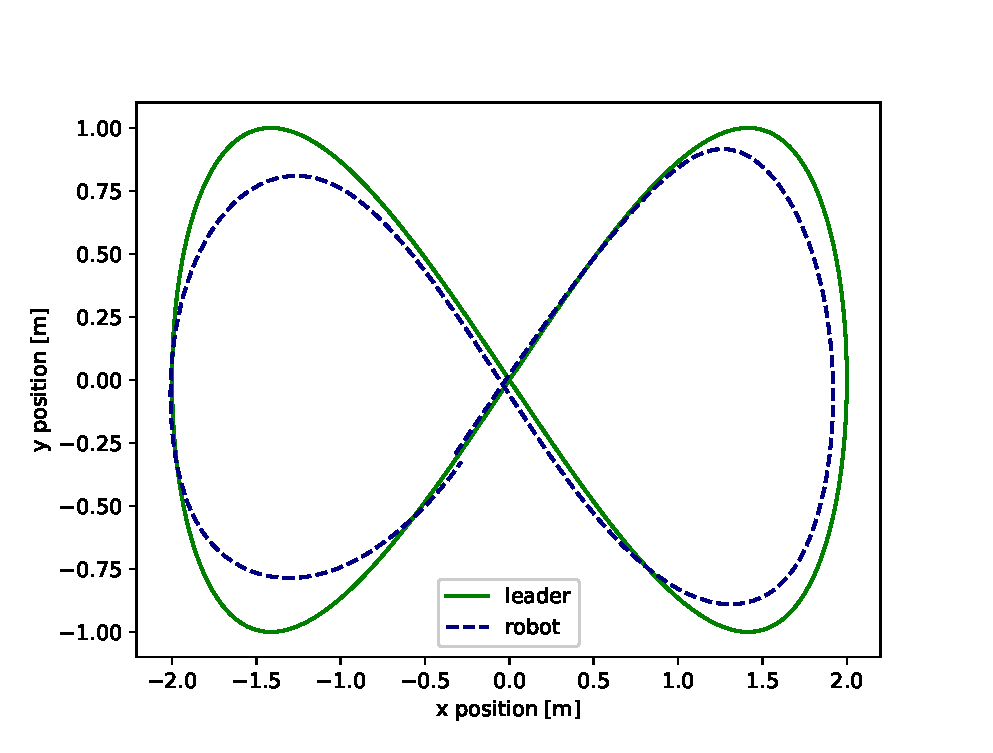
\includegraphics[width=0.97\linewidth]{images/Wft_5kg.eps}}
  \\
    \hspace*{-1.5em}
  \subfloat[ \label{rw1b}]{%
        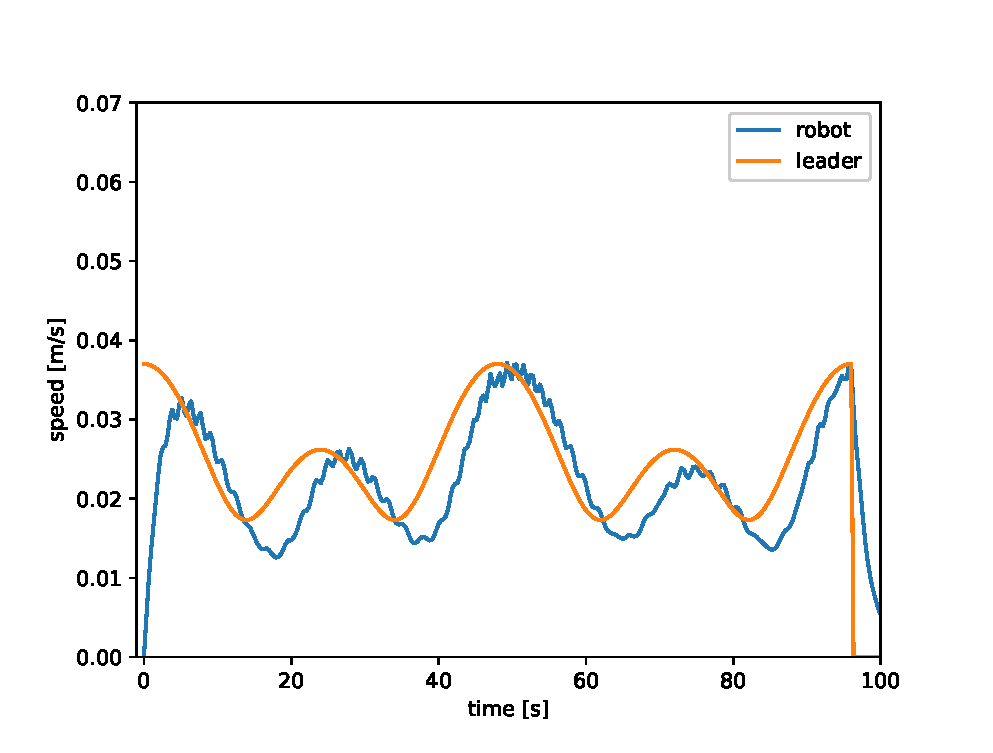
\includegraphics[width=0.49\linewidth]{images/Wft_5.0kg_leader_robot_speed.eps}}
    \vspace*{-1.1em}
  \subfloat[ \label{rw1c}]{%
        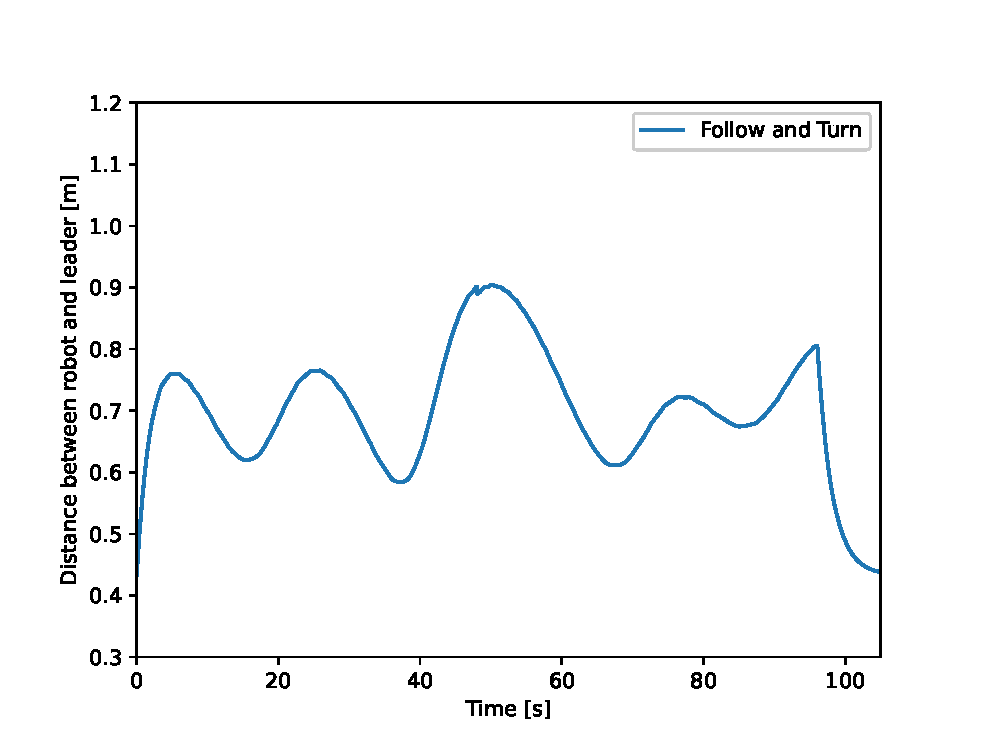
\includegraphics[width=0.49\linewidth]{images/Wft_5kg_distance.eps}}
    \hspace*{-1.5em}
    \vspace*{1.1em}
  \caption{Simulation results with the oxygen tank: the lemniscate trajectory is shown on (a) with the selected strategy \textit{Follow the thread}. (b) Speed profiles of the patient-leader and the robot-follower. (c) Distance between the patient and the robot while traversing the trajectory.}
  \label{fig:validationwithtank} 
\end{figure}


We added on the Webots simulation a 5 kg mass on top of our model, and adjusted the coefficients $c_v$ and $c_{\alpha}$ for the  \textit{Follow the thread}  control strategy.  Results are consistent with the outcomes shown previously on Figures~\ref{fig:simulationresults} and~\ref{fig:realworldresults}.  In Figure~\ref{fig:validationwithtank} it can be seen that the shape of the trajectory follows the patient smoothly, the speed profile also follows closely the leader speed, and finally the distance between the patient and the robot is maintained within the safe boundaries.  The obtained metrics are 0.2223 for m.t.d. and 1.1068 for t.t.d. which shows that the following behavior is achieved and verifies, from the simulation perspective, the initial feasibility of the control strategy considering the addition of the oxygen tank.

\section{Discussion}
\label{discussion}

From the leader and robot trajectories in Figure~\ref{fig:simulationresults}(a to d), both strategies exhibits basic following behavior.  However, \textit{Rotate and go} on Figure~\ref{fig:simulationresults}(b,d) generates a more irregular trajectory, due to the two stage movement algorithm.   

Regarding algorithms parameters, the simulation shows that for \textit{Follow the thread}, a low $c_{\alpha}$  means that the robot is slow to turn and makes wider turns, providing a smoother trajectory.  On the other hand, for low $c_v$ values, the robot tends to lag behind the leader when it is going in a straight line.  The highlighted values on Table~\ref{tab:simulationmetricsrg} show the best configuration found.  

For the \textit{Rotate and go} configuration, the parameter $c_r$ affects the dynamic behavior of the robot which needs to be adjusted accordingly.  Lastly, increasing the $Dt_{off}$ from 0.05 to 0.10 made the vehicle less prone to fall behind and produces a better following profile.
%For the \textit{Rotate and go} configuration, a high $c_r$ was important so the robot can turn quickly to point to the leader, but high values of $c_r$ and $c_v$ should be avoided, which may lead to dynamical issues with the inertia affecting the forward direction and missing the leader.  Lastly, increasing the $Dt_{off}$ from 0.05 to 0.10 made the vehicle less prone to fall behind and results in a better following profile.


%From the leader and robot trajectories in Figure \ref{fig:sim_ft_cv15_cr15}, we can see that the robot using \textit{Follow the thread} control exhibits basic following behavior. Deviation occurs when the leader trajectory turns with a tight radius. Comparing different simulations using different values of $c_{\alpha}$, we can also see that the robot tends to miss or cut corners when the leader turns, depending on the value of this constant (figures \ref{fig:sim_ft_cv15_cr5}, \ref{fig:sim_ft_cv15_cr10} and \ref{fig:sim_ft_cv15_cr15}). When $c_{\alpha}$ is low, the robot is slow to turn and makes wider turns, and when it is high, it can turn sharply as soon as the leader starts turning, so it will "cut" the curve. 

%Is was also found that with low $c_v$ values, the robot tends to lag behind the leader when it is going in a straight line, and as a consequence, when the leader turns, the follower is further away and has to make a sharper turn to keep following the leader. Again, a very low values of $c_v$ makes the follower "cut corners", as can be seen in figure \ref{fig:sim_ft_cv5_cr20}.

%The rotateand go We see that this strategy also exhibits a following behavior, although in a more irregular path, as expected, due to the two stage movement algorithm. In this case we evaluated the effects of the constants $c_v$, $c_r$ and $Dt_{off}$. 

%We found that it is important to have a high $c_r$ so the robot turns quickly to point to the leader, or otherwise, as the leader turns, the robot never stops rotating since it takes too much time to get to the point where it can go forward. Therefore, if the leader makes a long turn, the robot never stops rotating and stops following the leader (figure \ref{fig:rgv_cv20_cr5_dr05}).

%However, a very high $c_r$ causes a different issue. When the robot finally points at the leader and starts going forward, if it was rotating too fast, the inertia of the wheels and the robot itself affect the forward movement of the vehicle, which can turn sideways as it tries to go forward in a straight line, diverting the robot from its intended path. A similar thing happens with a very high $c_v$: when the robot stops to rotate, its inertia prevents it from stopping completely and its path is affected as a consequence. This can be seen in figure \ref{fig:rgv_cv35_cr20_dr10}.

%Lastly, we found that calibrating the $Dt_{off}$ parameter also has positive effects in the following performance, since it leaves more margin for the robot to go forward before rotating to point at the leader again. Increasing the $Dt_{off}$ from 0.05 to 0.10 made the vehicle less prone to fall behind and results in a better following (see figure \ref{fig:rg_dt_comp}).



%Both behaviors are described by figures \ref{fig:ft_speed_1} and \ref{fig:rg_speed_1}, which show the speed of the leader and the robot over time.


%When we measured the robot-leader distance over time, we see another significant between the two strategies. As mentioned before, using \textit{Rotate and go}, as the robot rotates, the leader can get further away. Figures \ref{fig:ft_vs_rg_dist} and \ref{fig:ft_vs_rg_dist_hist} show the distance over time and the distribution of distances for each strategy, respectively. 



In line with the simulated results, a similar behavior was found on the experiments performed inside the Motion Capture Lab, and the robot exhibits following behavior for both control strategies as shown on Figure~\ref{fig:realworldresults}.   Although the parameter values obtained from the simulation had to be readjusted for the real world scenario, the relative relation between them was maintained and that helped to narrow the parameter search space.


%We can see that, again, the robot exhibits following behavior. The trajectories in the figures mentioned above show a similar behavior to the one in the software simulation, for both control strategies.

%As in the software simulation, we also evaluated the influence of the algorithm parameters in the robot movement, using the hardware prototype. Figures \ref{fig:ft1_cap_leader_robot} and \ref{fig:ft2_cap_leader_robot} show the robot and leader movement using different values for $c_{\alpha}$. As we have seen in the simulation, a higher $c_{\alpha}$ makes the robot tend to "cut corners" (figure \ref{fig:ft2_cap_leader_robot}).

%For the \textit{Rotate and go} strategy, we compared how different values of $Dt_{off}$ behaved. As we can see in figure \ref{fig:ft2_cap_leader_robot}, a higher $Dt_{off}$ makes the robot less sensitive to leader turns, so the robot has time to move forward and follow the shape of the curve more accurately. 

As expected, the \textit{Rotate and go} strategy performs a \textit{stop and go} movement, since the vehicle completely stops when rotating to face the leader. This is shown on the speed profiles in Figure~\ref{fig:simulationresults}(c,d) as well as on the real experiment on Figure~\ref{fig:realworldresults}(c,d).    The smoother movement of the \textit{Follow the thread} algorithm is an additional desired goal, since it can be perceived as less violent or unexpected. %Additionally, when the vehicle stops to rotate, if the leader continues moving, when going forward, the robot might need to accelerate sharply to catch up with the leader, resulting in a sudden movement that can be disturbing for a medical patient or a doctor in the middle of a treatment.

%As it was mentioned before, a smoother movement, with no sudden accelerations, can be desired in the environment where the robot is expected to function, so the \textit{Rotate and go} strategy is better in this respect.

%Another thing to note is that, since the robot has inertia when it tries to stop and rotate (in \textit{Rotate and go}), its speed never gets to  zero as it rotates on its axis. This can also be an issue when following the leader, since the robot can be pushed off its course due to its own movement. 


%As in the simulation, we also see differences in the robot-leader distance over time. The \textit{Rotate and go} strategy performs worse in this respect, reaching higher maximum distances and a higher average distance to the leader (table \ref{tab:cap_ft_vs_rg_dist_table}).

Finally, regarding the Robot-leader distance r.l.d., the \textit{Rotate and go} strategy results in a less stable distance (higher standard deviation), with higher maximum values, both on the simulated (Figure~\ref{fig:simulationresults}(e)) and on the real world scenario (Figure~\ref{fig:realworldresults}(e)).  This can be specially problematic if we consider the cannula connecting the oxygen tank to the patient, as the cannula has a limited length.  

%These values are also compared in Table \ref{tab:cap_ft_npd_table} and Table~\ref{tab:cap_rg_npd_table}.  

\subsection{Clinical Assessment} 
\label{clinical}

No amount of metrics are enough to evaluate if the robot is a viable solution for this problem or not, without the feedback and the evaluation of the people that are going to physically make use of it. 

ALPI is a non-profit civil association located in Buenos Aires, Argentina, that provides neuromotor rehabilitation for pediatric and adult patients. It was founded in 1943 with the main focus of treating children with poliomyelitis, and has since expanded to deal with all kinds of related diseases. 

Four professional care-givers from ALPI  were invited to test and evaluate the controlling strategy on the prototype.  A live demonstration of the robot working and following a moving person was performed.

In the demonstration, the robot design was outlined and an explanation was given on how the robot worked, how it was built and how to operate it. Both control strategies were explained, along with the main superficial differences between them. 

Afterwards, health care professionals were invited to use the robot themselves, simulating they were the patient being followed. They were allowed to switch between the two control strategies to evaluate both of them, and made different tests, one walking along standardized trajectory marked on the floor and another one walking freely along the available space of the Motion Capture Lab. They used the robot freely to get a general idea of how it behaved, and how it could be used in the rehabilitation process. After all evaluations were finished, various aspects of the vehicle prototype were discussed and then a survey was handed out to document their experience with the robot, get their expert opinion on how the two strategies compared against each other, and what other improvements were needed in order to deliver a fully usable product.  Survey questions and their averaged numerical evaluations are provided in Table~\ref{tab:alpi_q_table_1}.

\begin{table*}[t]
\begin{center}
\begin{tabular}[!t]{|c|c|}
\hline
Question & Avg. answer \\
\hline
How would you qualify, from 1 to 5, your overall experience with \textit{Follow the thread}? (1:Bad, 5:Excellent)  & 5.0\\
\hline
How safe would a patient be, from 1 to 5, being followed by the robot using the \textit{Follow the thread} strategy? (1:Very unsafe, 5:Very safe)  & 4.25\\
\hline
How would you qualify, from 1 to 5, your overall experience with \textit{Rotate and go}? (1:Bad, 5:Excellent)  & 3.5\\
\hline
How safe would a patient be, from 1 to 5, being followed by the robot using the \textit{Rotate and go} strategy? (1:Very unsafe, 5:Very safe) & 3.25\\
\hline
\end{tabular}
\captionof{table}{Answers to survey questions.}
\label{tab:alpi_q_table_1}
\end{center}
\end{table*}

According to their answers, and the discussion we had after testing the robot, the general opinion was that the \textit{Follow the thread} strategy was safer and more convenient for the task. In the survey, when asked \textit{Which of the two strategies is more effective at following the patient in a rehabilitation exercise?}, all 4 people responded that \textit{Follow the thread} is "much better".

The main concern with the \textit{Rotate and go} strategy was that having to wait for the robot to rotate before moving forward might be unsafe, as the patient could move away from it and compromise the cannula connecting him or her to the oxygen tank. This issue was identified during our own tests, and was not mentioned when explaining the following mechanism to the doctors, to avoid skewing them. They independently identified this problem, and emphasized that it could be a great source of discomfort for the patient.

Another aspect that was remarked from the \textit{Follow the thread} strategy is that since it had a smoother movement, with no sudden stops or accelerations, it was favorable for the stability of the robot in order to carry the heavy oxygen tank.

Two needed security measures were also brought up by the ALPI team. Firstly, the need to add some mechanism for obstacle avoidance. They mentioned the need to have sensors to detect if the robot was about to hit something (specially the patient), and stop immediately, apart from what the control strategy indicated. Secondly, they recognized that some patients have very weak stability, and might fall down or take a step back, towards the robot, so it should be able to automatically move away from the patient, in order not to become another obstacle for him or her. 

In order to have more information for the next steps in the development of the robot, we asked for their advise to design the mechanism to attach the threads to the patient being followed. Two ideas were proposed: a belt strapped to the patient waist, or a clasp tied to the clothes of the patient, also near its waistline. The waist is a good attachment point, since it is relatively more stable when the patient moves, compared to its hands or legs, that may make sudden movements and confuse the robot sensors. 


\section{Conclusion and Future Work}
\label{conclusion}

From the practical experiments, it is verified that both algorithms ensuing the \textit{following behavior}  in the task of tracking the patient along a lemniscate-shaped trajectory. This following behavior is accomplished with a simple mechanism, a characteristic that significantly keep the price of the device low, putting it within reach of many medical institutions on developing nations.

Each control strategy has its advantages, but according to various metrics described in this work, the \textit{Follow the thread} strategy had a more desirable behavior, as it tended to follow the leader from a closer distance at all times, while moving in a smooth and predictable way. 

Insightful feedback is gathered from healthcare professionals from ALPI, who provided invaluable data to evaluate the solution. Over all, they highlight the \textit{Follow the thread} strategy as being the safer and more effective one. Most importantly, they also validated the research and were enthusiast about the direction of the project. They proposed a series of improvements and next steps after seeing the prototype in action.

As described in the beginning, it is essential to involve stakeholders such as patients, doctors, nurses, and any other professionals involved in the rehabilitation process early in the design roadmap. They are the ones who understand the problem better than anyone else, and will be the end users of any developed product, as long as it is useful for them.

%The staff at ALPI was enthusiastic about helping in the development of the robot, and their encouragement and support are key reasons to take this project forward.  There are yet many challenges ahead, but these initial results are promising about the viability to develop a real world solution that can improve the quality of life of many people through the use of technology and engineering. 


% \subsection{Validation carrying the oxygen tank}

% In order to advance towards the next step, we performed an additional simulated experiment to validate whether or not the selected algorithm could be extended to  handle the oxygen tank.  ALPI works with 5 kg oxygen tanks, which are manufactured locally.

% We added on the Webots simulation a 5 kg mass on top of our model, and adjusted the coefficients $c_v$ and $c_{\alpha}$ for the  \textit{Follow the thread}  control strategy.  Results are consistent with the outcomes shown previously on Figures~\ref{fig:simulationresults} and~\ref{fig:realworldresults}.  In Figure~\ref{fig:validationwithtank} it can be seen that the shape of the trajectory follows the patient smoothly, the speed profile also follows stringently the leader speed, and finally the distance between the patient and the robot is maintained within the safe boundaries.  The obtained metrics are 0.2223 for m.t.d. and 1.1068 for t.t.d. which shows that the following behavior is achieved and verifies, from the simulation perspective, the initial feasibility of the control strategy considering the addition of the oxygen tank.

\subsection{Future Work}
%A following mechanism has been designed and implemented in a hardware prototype. The mechanism, along with the two control algorithms, has shown promise to be a viable solution to implement in a functioning robot that ALPI, or any other medical institution, can use in their every day exercises with COPD patients. 

The next steps for this project is to scale and iterate the design towards the desired solution, using the data obtained from this experiments and the feedback from care-givers.

\begin{itemize}
    \item Redesign the active spring control mechanism in order to hold the motor temperature in its operational range.
    \item An easy and safe interaction between the patient, the operator and the robot. How to communicate the state of the robot to the operator, how to control and manipulate the robot in an effective and user-friendly way.
    \item Safety measures to keep the patient and the care-giver safe when using the robot. Not only safe from the robot movement, but also from its electronic components.
    \item An obstacle avoidance subsystem. This necessity is emphasized by the personnel from ALPI. The robot should have mechanisms in place to deal with emergency situations, and under no circumstance it can hit the patient or the doctor operating it.
    \item Achieve a battery autonomy that makes the robot useful throughout a complete pulmonary rehabilitation exercise. It is crucial for its usefulness to be able to hold a charge for this period of time, along with the ability to quickly swap batteries if the vehicle will be continually used with different patients.
\end{itemize}{}


% if have a single appendix:
%\appendix[Proof of the Zonklar Equations]
% or
%\appendix  % for no appendix heading
% do not use \section anymore after \appendix, only \section*
% is possibly needed

% use appendices with more than one appendix
% then use \section to start each appendix
% you must declare a \section before using any
% \subsection or using \label (\appendices by itself
% starts a section numbered zero.)
%

% use section* for acknowledgment
\section{Acknowledgments}
This project is part of a joint collaboration between ALPI organization and the ITBA University.  Authors would like to thank thoughtfully for the initiative and support given by ALPI, and to the Director of Rehabilitation Technology Dra. Mercedes Molinuevo.  Additionally, authors would also like to offer tremendous gratitude to Natalia Nerina Meda, Soledad Suriá, Eduardo Etcheverry and Sergio Carlos Franco, for the idea of this project and for their invaluable help and enthusiasm to move this project forward.


\section*{Conflict of Interest Statement}
The authors declare that the research was conducted in the absence of any commercial or financial relationships that could be construed as a potential conflict of interest.


% Can use something like this to put references on a page
% by themselves when using endfloat and the captionsoff option.
\ifCLASSOPTIONcaptionsoff
  \newpage
\fi



% trigger a \newpage just before the given reference
% number - used to balance the columns on the last page
% adjust value as needed - may need to be readjusted if
% the document is modified later
%\IEEEtriggeratref{8}
% The "triggered" command can be changed if desired:
%\IEEEtriggercmd{\enlargethispage{-5in}}

% references section

% can use a bibliography generated by BibTeX as a .bbl file
% BibTeX documentation can be easily obtained at:
% http://mirror.ctan.org/biblio/bibtex/contrib/doc/
% The IEEEtran BibTeX style support page is at:
% http://www.michaelshell.org/tex/ieeetran/bibtex/
\bibliographystyle{IEEEtran}
\bibliography{alpibot}

%
% <OR> manually copy in the resultant .bbl file
% set second argument of \begin to the number of references
% (used to reserve space for the reference number labels box)
%\begin{thebibliography}{1}

%\bibitem{IEEEhowto:kopka}
%H.~Kopka and P.~W. Daly, \emph{A Guide to \LaTeX}, 3rd~ed.\hskip 1em plus
%  0.5em minus 0.4em\relax Harlow, England: Addison-Wesley, 1999.

%\end{thebibliography}

% biography section
% 
% If you have an EPS/PDF photo (graphicx package needed) extra braces are
% needed around the contents of the optional argument to biography to prevent
% the LaTeX parser from getting confused when it sees the complicated
% \includegraphics command within an optional argument. (You could create
% your own custom macro containing the \includegraphics command to make things
% simpler here.)\begin{IEEEbiographynophoto}
%\begin{IEEEbiography}[{\includegraphics[width=1in,height=1.25in,clip,keepaspectratio]{mshell}}]{Michael Shell}
% or if you just want to reserve a space for a photo:

%\begin{IEEEbiography}[{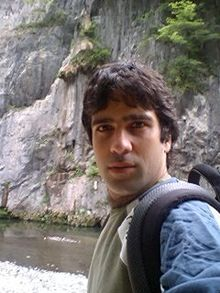
\includegraphics[width=1in,height=1.25in,clip,keepaspectratio]{ramele}}]{Rodrigo Ramele}
%currently works at the Centro de Inteligencia Computacional (CIC), ITBA University, Buenos Aires, Argentina. Rodrigo does research in Brain Computer Interfaces, Artificial Intelligence, Signal Processing and Robotics.
%\end{IEEEbiography}
%
%% if you will not have a photo at all:
%\begin{IEEEbiography}[{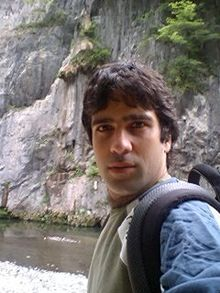
\includegraphics[width=1in,height=1.25in,clip,keepaspectratio]{santos}}]{Juan Miguel Santos}
%is the Director of the Centro de Inteligencia Computacional (CiC) of ITBA University in Buenos Aires, Argentina, where he works in three different areas: robotics development, reinforcement learning and brain-computer interfaces.  In the first two lines he works since 1993 developing and constructing robots, national and international robotics conferences and international peer-review journals.  Currently developing a new development line based on SLAM to autonomous robots.
%\end{IEEEbiography}


% insert where needed to balance the two columns on the last page with
% biographies
%\newpage

% You can push biographies down or up by placing
% a \vfill before or after them. The appropriate
% use of \vfill depends on what kind of text is
% on the last page and whether or not the columns
% are being equalized.

%\vfill

% Can be used to pull up biographies so that the bottom of the last one
% is flush with the other column.
%\enlargethispage{-5in}



% that's all folks
\end{document}